\documentclass[9pt]{article}
\usepackage[english]{babel}
\usepackage{amsmath,amsthm}
\usepackage{amsfonts}
\usepackage{graphicx}
\usepackage[margin=0.2in]{geometry}
\newcommand{\setlinespacing}[1]{\setlength{\baselineskip}{#1 \defbaselineskip}}
\newcommand{\doublespacing}{\setlength{\baselineskip}{2.0 \defbaselineskip}}
\newcommand{\singlespacing}{\setlength{\baselineskip}{\defbaselineskip}}
\newcommand{\A}{{\cal A}}
\newcommand{\h}{{\cal H}}
\newcommand{\s}{{\cal S}}
\newcommand{\W}{{\cal W}}
\newcommand{\BH}{\mathbf B(\cal H)}
\newcommand{\KH}{\cal  K(\cal H)}
\newcommand{\Real}{\mathbb R}
\newcommand{\Complex}{\mathbb C}
\newcommand{\Field}{\mathbb F}
\newcommand{\RPlus}{[0,\infty)}
\newcommand{\norm}[1]{\left\Vert#1\right\Vert}
\newcommand{\essnorm}[1]{\norm{#1}_{\text{\rm\normalshape ess}}}
\newcommand{\abs}[1]{\left\vert#1\right\vert}
\newcommand{\set}[1]{\left\{#1\right\}}
\newcommand{\seq}[1]{\left<#1\right>}
\newcommand{\eps}{\varepsilon}
\newcommand{\To}{\longrightarrow}
\newcommand{\RE}{\operatorname{Re}}
\newcommand{\IM}{\operatorname{Im}}
\newcommand{\Poly}{{\cal{P}}(E)}
\newcommand{\EssD}{{\cal{D}}}
\newcommand{\field}[1]{\mathbb{#1}}
\newcommand{\C}{\field{C}}
\newcommand{\R}{\field{R}}
\newcommand{\script}[1]{\mathcal{#1}}
\newcommand{\fall}{\; \forall \;}
\newcommand{\exts}{\; \exists \;}
\newcommand{\mbf}[1]{\mathbf{#1}}
\newcommand{\binomial}[2]{\biggl( \begin{array}{c}  #1 \\ #2  \\ \end{array} \biggr) }
\newcommand{\fderiv}[2]{ \frac{d}{ d #1} \: #2}
\newcommand{\sderiv}[2]{ \frac{d^2}{ d^2 #1} \: #2}
\newcommand{\pfderiv}[2]{ \frac{\partial}{ \partial #1} \: #2}
\newcommand{\psderiv}[2]{ \frac{\partial^2}{ \partial^2 #1} \: #2}
\newcommand{\mat}[1]{\mathbf{#1}}
\DeclareSymbolFont{AMSb}{U}{msb}{m}{n}
\DeclareMathSymbol{\dblz}{\mathalpha}{AMSb}{"5A}
\DeclareMathSymbol{\dblr}{\mathalpha}{AMSb}{"52}
\DeclareMathSymbol{\dblt}{\mathalpha}{AMSb}{"54}
\DeclareMathSymbol{\dblq}{\mathalpha}{AMSb}{"51}
\DeclareMathSymbol{\dbln}{\mathalpha}{AMSb}{"4E}
\DeclareMathSymbol{\dblf}{\mathalpha}{AMSb}{"46}
\DeclareMathSymbol{\dblc}{\mathalpha}{AMSb}{"43}
\DeclareMathSymbol{\dbld}{\mathalpha}{AMSb}{"44}
\theoremstyle{plain}
\newtheorem{thm}{Theorem}[section]
\newtheorem{cor}[thm]{Corollary}
\newtheorem{lem}[thm]{Lemma}
\newtheorem{prop}[thm]{Proposition}
\theoremstyle{definition}
\newtheorem{defn}{Definition}[section]
\theoremstyle{remark}
\newtheorem{rem}{Remark}[section]
\numberwithin{equation}{section}
\renewcommand{\theequation}{\thesection.\arabic{equation}}
\begin{document}
\title{Regression of KL Software Distribution   }
\author{KL Software Libraries}
\date{Thu Jun 12 03:06:36 2014
}
\maketitle
\textbf{ KL Library test output.  This LaTex file and the associated diagrams are produced by the KL software libraries.}
\subsubsection{Multiclass Support Vector Machine }
\begin{itemize}
\item Number or training points = 1024
\item Feature dimension = 3
\item Number or classes = 3
\end{itemize}
{The mean vectors of the 3 classes}

$\mu_1 = \left(
\begin{array}{
ccc}
+1.90000 & +0.10000 & +0.10000 \\
\end{array}
\right)$ \newline 

$\mu_2 = \left(
\begin{array}{
ccc}
+0.10000 & +1.90000 & +0.10000 \\
\end{array}
\right)$ \newline 

$\mu_3 = \left(
\begin{array}{
ccc}
+0.00000 & +0.00000 & +1.90000 \\
\end{array}
\right)$ \newline 

A random SPD covairance matrix is generated for each of the classes.\newline

$\rho_1 = \left(
\begin{array}{
ccc}
+4.211 & -0.025 & -0.434 \\
-0.025 & +3.080 & -0.373 \\
-0.434 & -0.373 & +3.121 \\
\end{array}
\right)$ \newline 

$\rho_2 = \left(
\begin{array}{
ccc}
+2.697 & +0.054 & -0.423 \\
+0.054 & +1.556 & +0.173 \\
-0.423 & +0.173 & +2.982 \\
\end{array}
\right)$ \newline 

$\rho_3 = \left(
\begin{array}{
ccc}
+2.031 & -0.029 & +0.462 \\
-0.029 & +4.365 & +0.459 \\
+0.462 & +0.459 & +2.314 \\
\end{array}
\right)$ \newline 

Verify $L_1$ condition number of covariance. The diagonal entries of the matrix have the form $(0.5 + U(0,1) )*dim(Dom(Cov))$
The lower-diagonal entries take the form $U(0,1) - 0.5$. 
The $L_1$ condition numbers are :
\begin{itemize}
\item +1.889
\item +2.532
\item +3.094
\end{itemize}
\includegraphics[width=10.0cm,height=10.0cm]{rv1_corr.pdf}

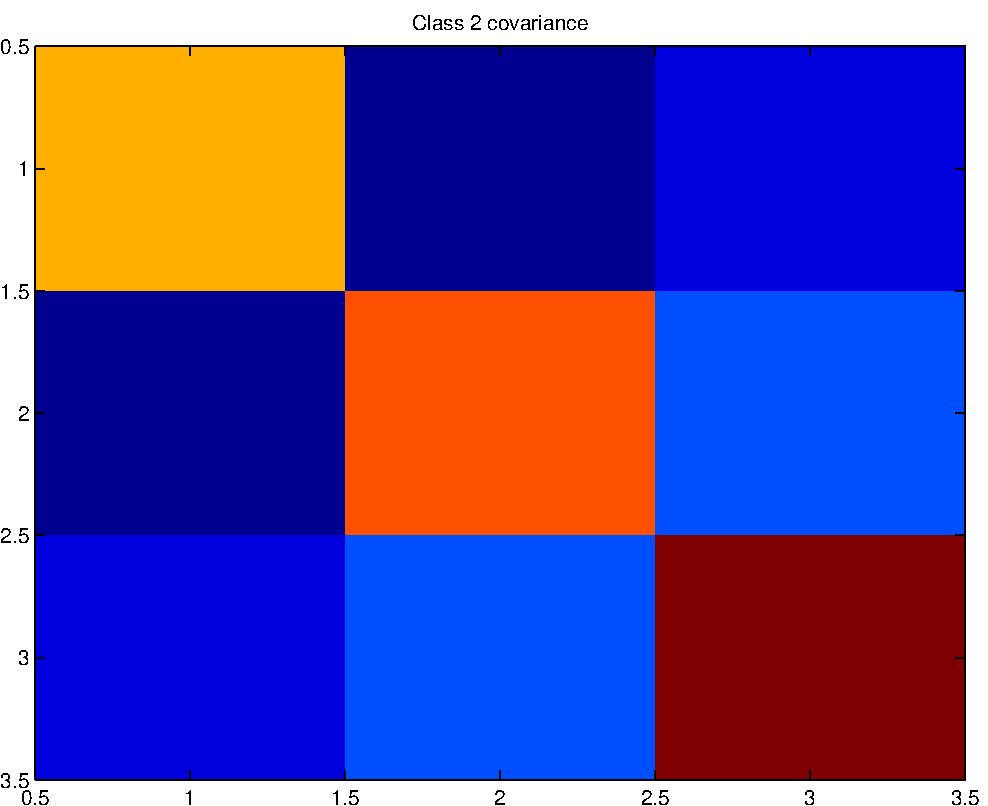
\includegraphics[width=10.0cm,height=10.0cm]{rv2_corr.pdf}

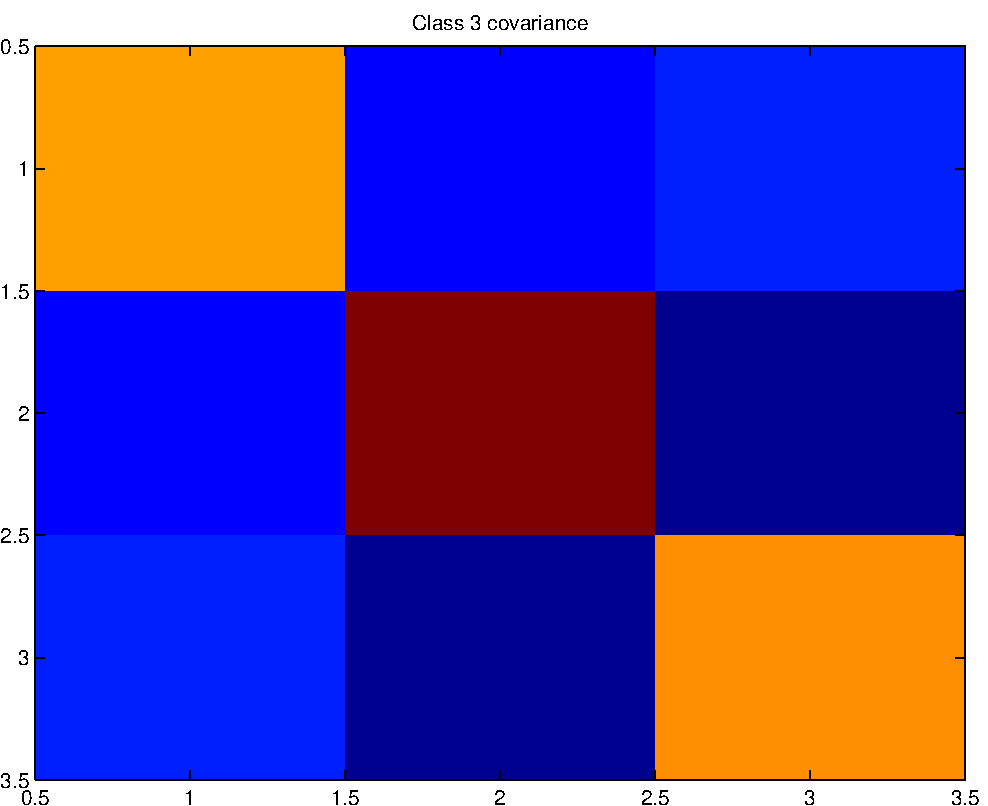
\includegraphics[width=10.0cm,height=10.0cm]{rv3_corr.pdf}

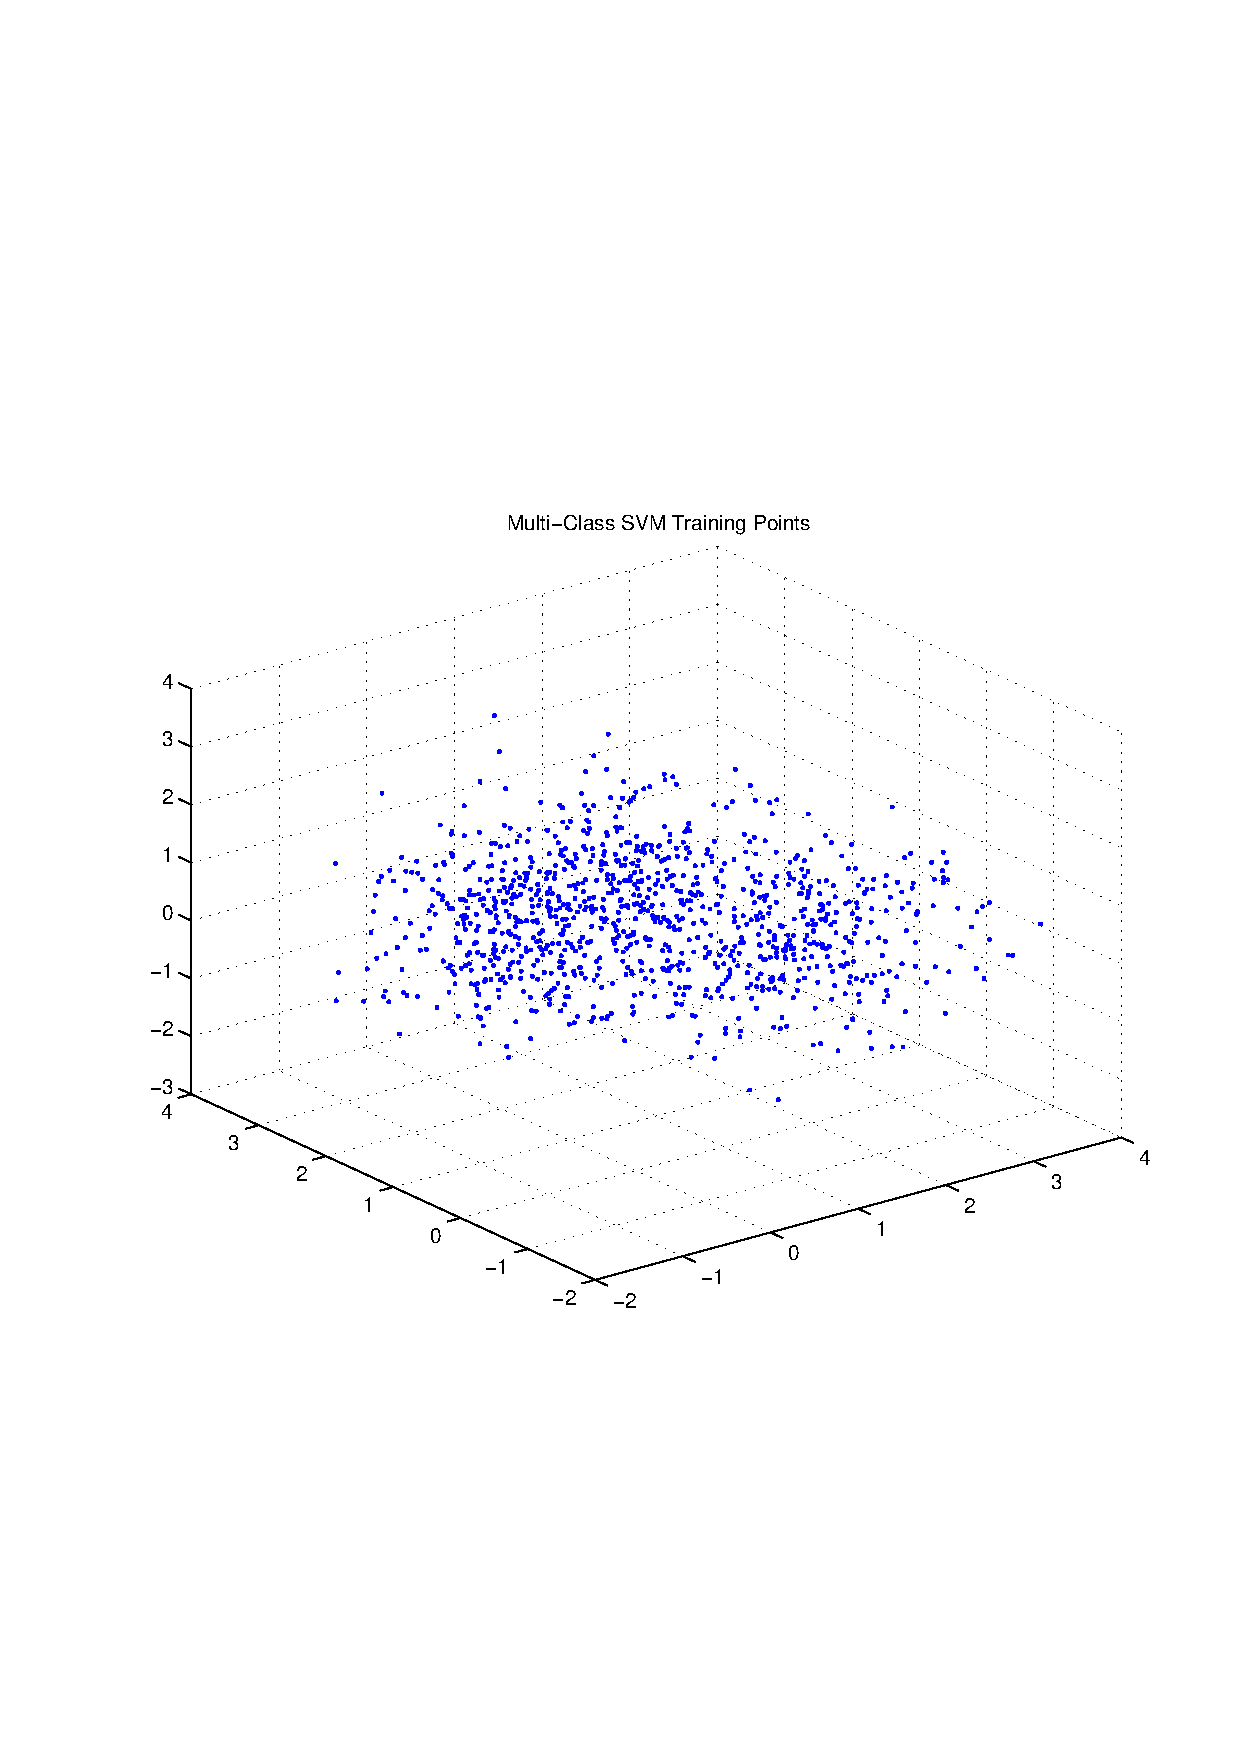
\includegraphics[width=10.0cm,height=10.0cm]{trainingPoints.pdf}

These are the SVM parameters - the RBF kernel is used\begin{itemize}
\item allOutlierFraction=0.05
\item mixingCoeff=0.3
\item smoThresh=1.0/10000.0
\item sigma=1
\end{itemize}
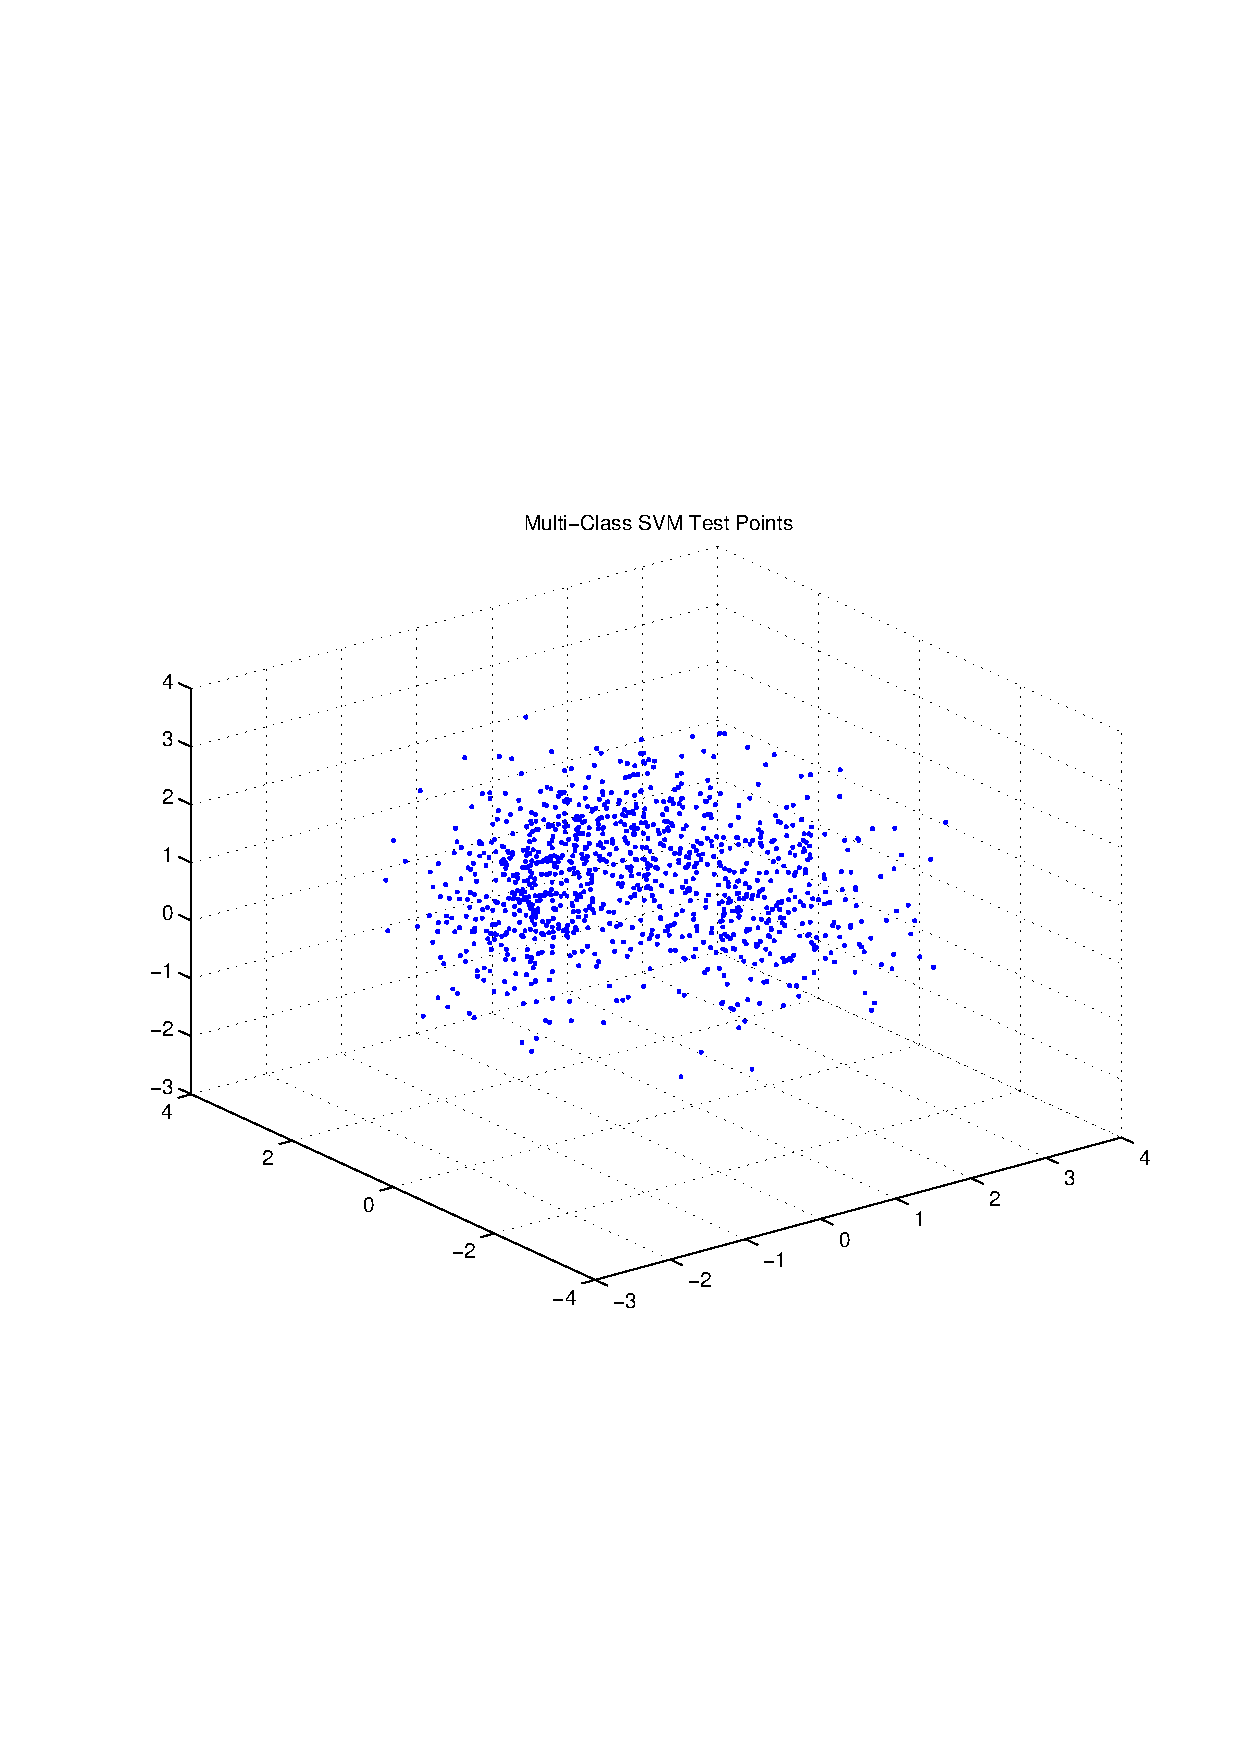
\includegraphics[width=10.0cm,height=10.0cm]{testPoints.pdf}

The marginal sample moments (mean var skew kurtosis) for training points.\newline
\begin{tabular}{ c |  c  c  c  c}
Feature & $\mu_1$ & $\mu_2$ & $\mu_3$ & $\mu_4$ \\
0 & +0.671 & +1.348 & +0.490& +2.578 \\
\hline
1 & +0.703 & +1.268 & +0.025& +2.109 \\
\hline
2 & +0.700 & +1.271 & +0.223& +2.337 \\
\hline
\end{tabular}
\newline
The marginal sample moments (mean var skew kurtosis) for test points.\newline
\begin{tabular}{ c | c  c  c  c}
Feature & $\mu_1$ & $\mu_2$ & $\mu_3$ & $\mu_4$ \\
0 & +0.678 & +1.267 & +0.648& +2.767\\
\hline
1 & +0.668 & +1.272 & +0.071& +2.109\\
\hline
2 & +0.723 & +1.199 & +0.192& +2.230\\
\hline
\end{tabular}\newline
\includegraphics[width=10.0cm,height=10.0cm]{classDiffs.pdf}

The error rate for this run is +0.114\newline
QueryPerformanceCounter  =  +6.183
\subsubsection{Matrix Quick Check <double>}
QueryPerformanceCounter  =  +0.052
\subsubsection{Linear Regression atan data 3x1}
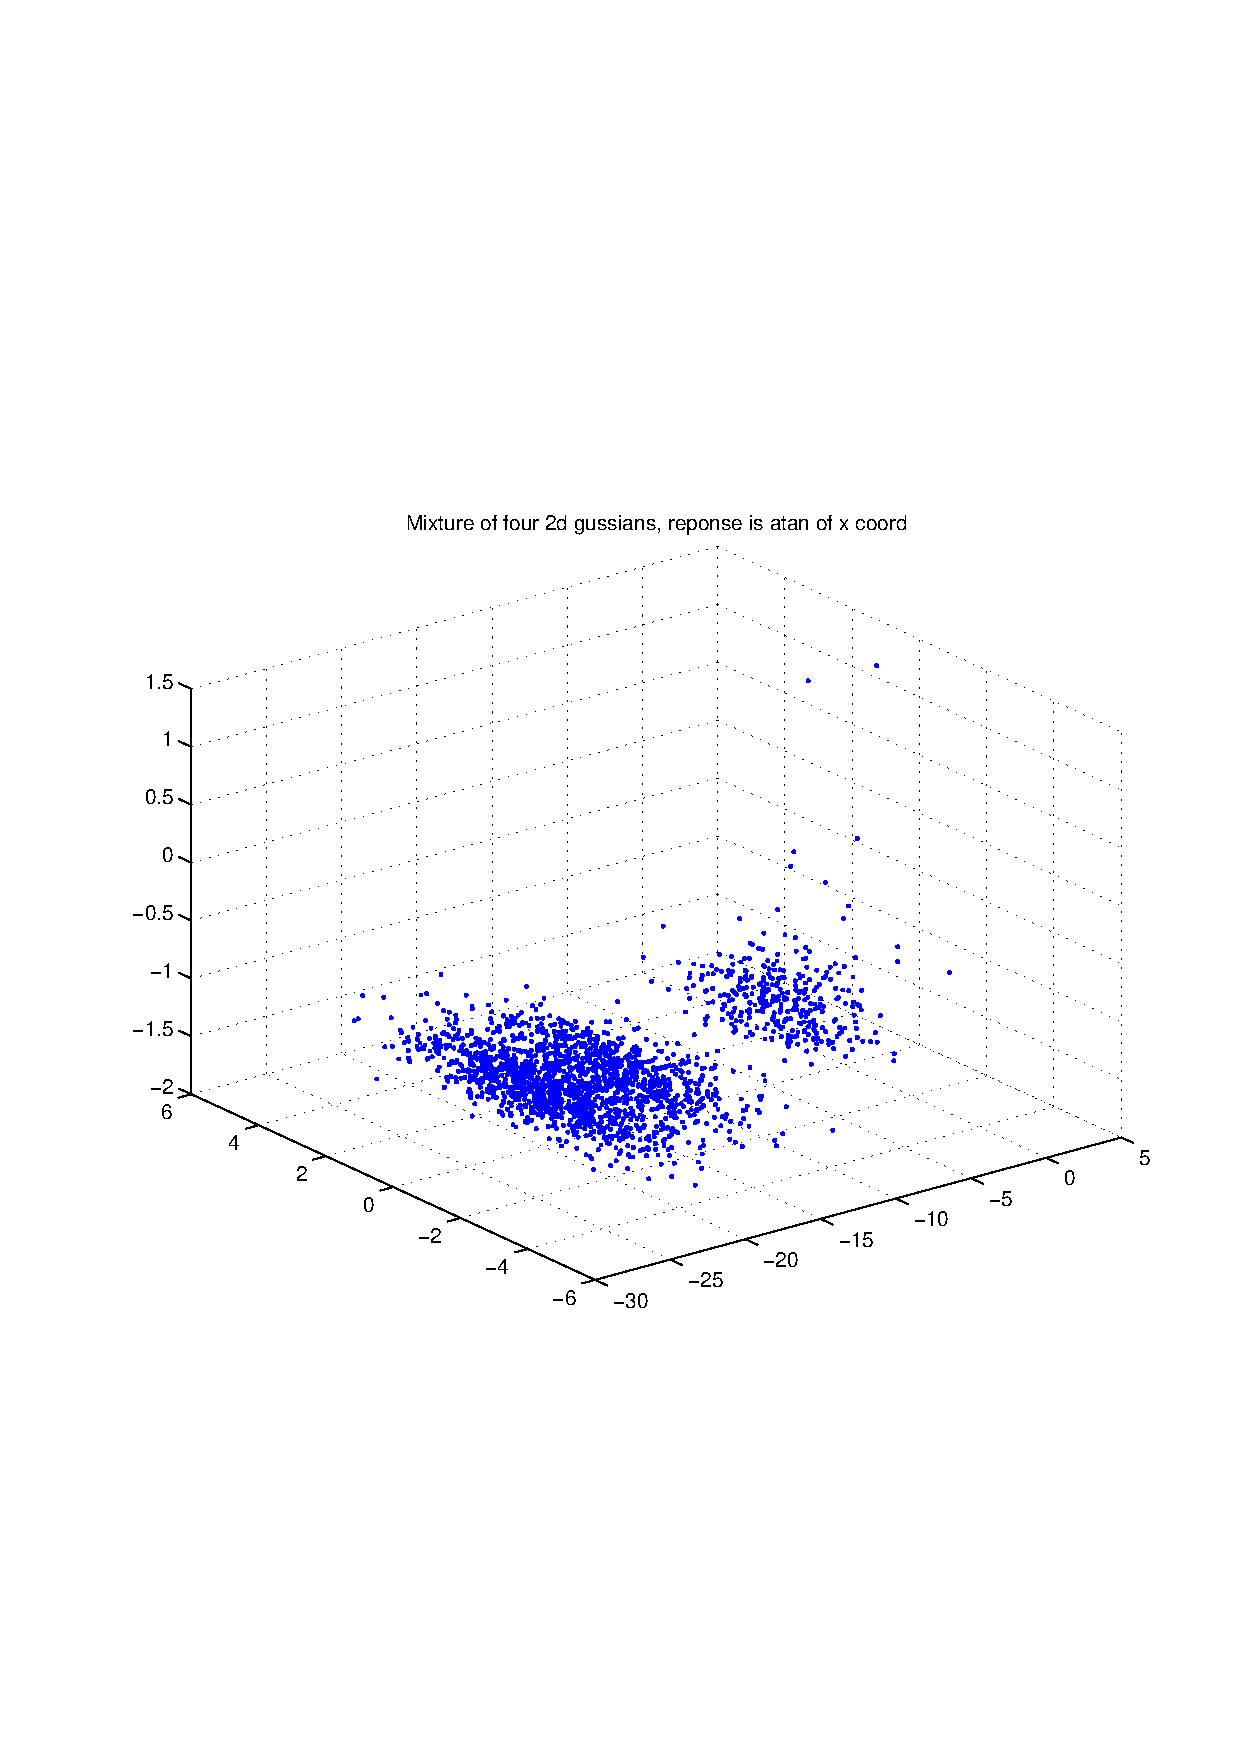
\includegraphics[width=10.0cm,height=10.0cm]{AtanDataSet.pdf}

\subsubsection{3 x 1 Linear Regression}
Sample size = 4000

Number of features = 3

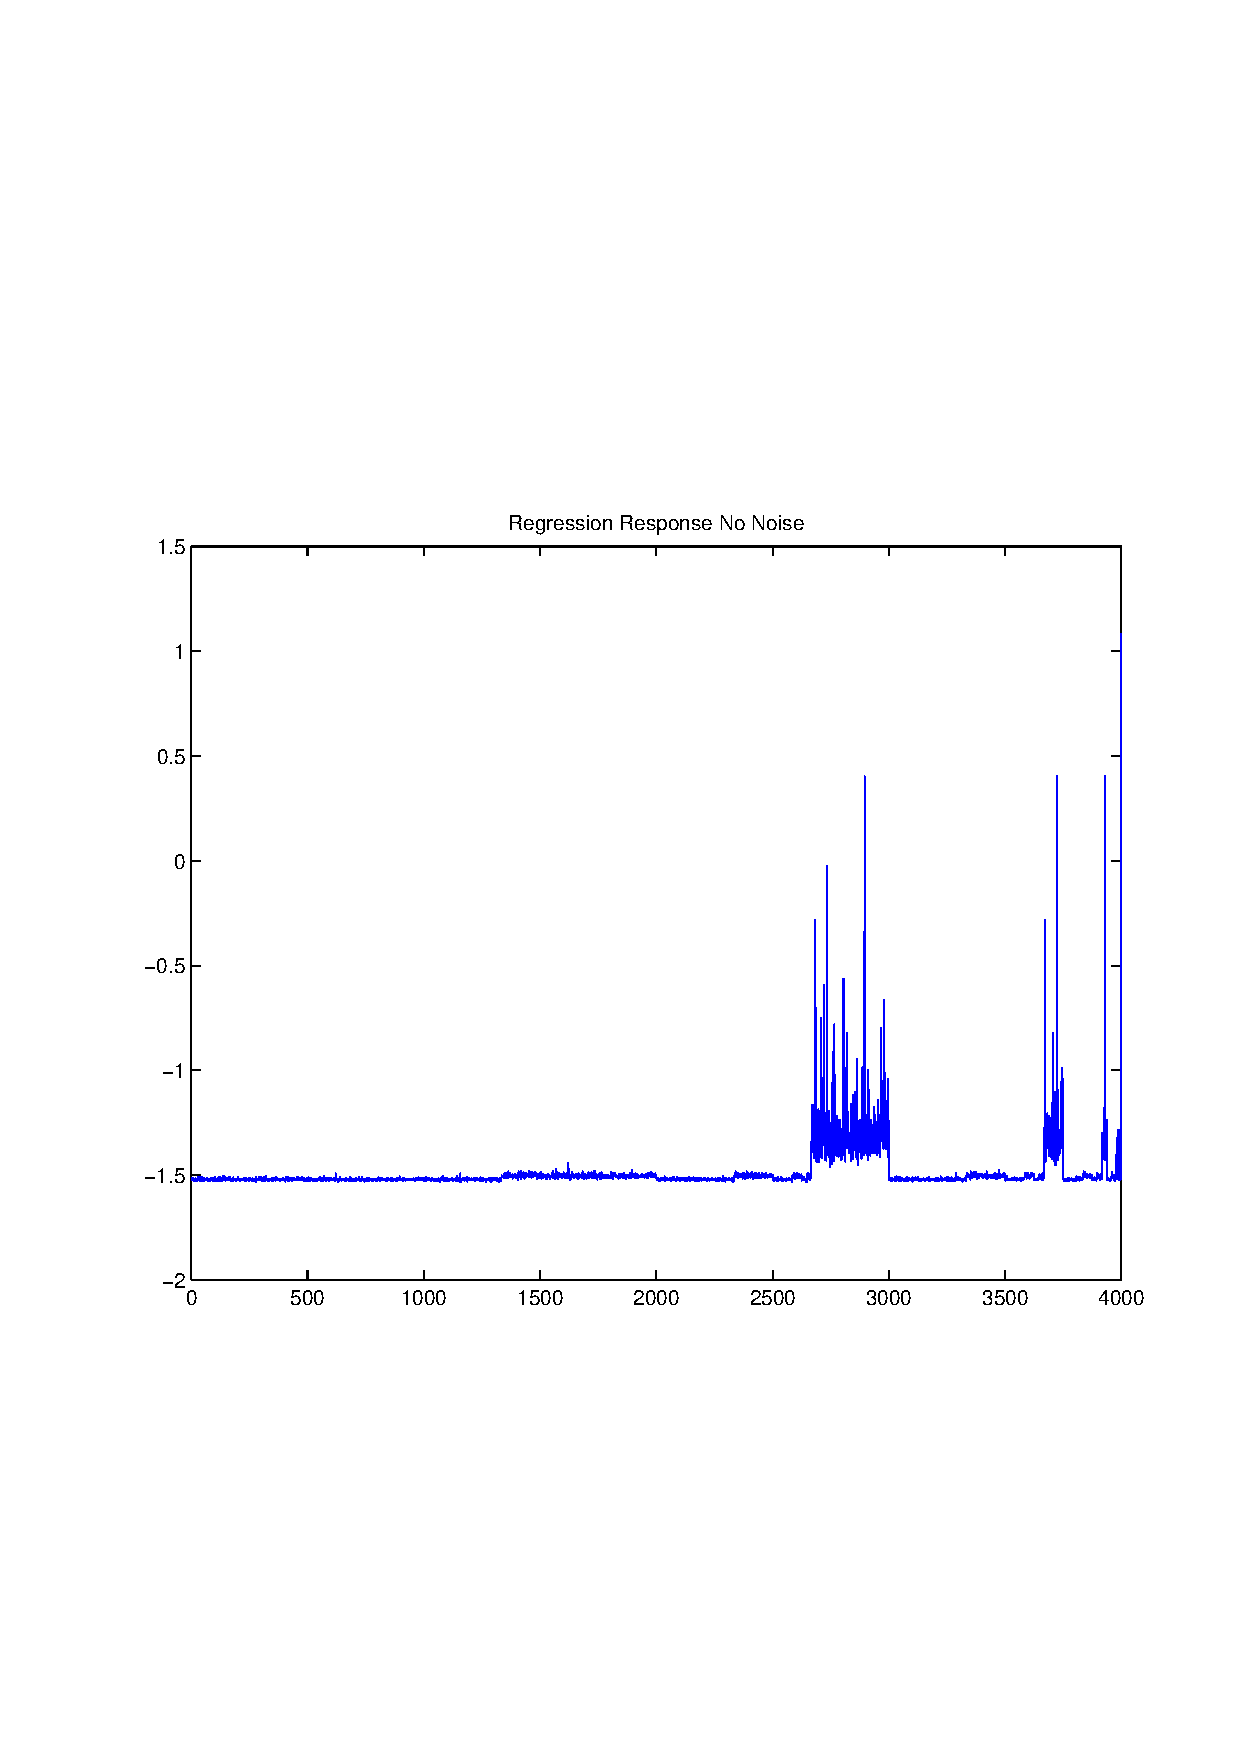
\includegraphics[width=10.0cm,height=10.0cm]{AtanDataSet_regression_response_no_noise.pdf}

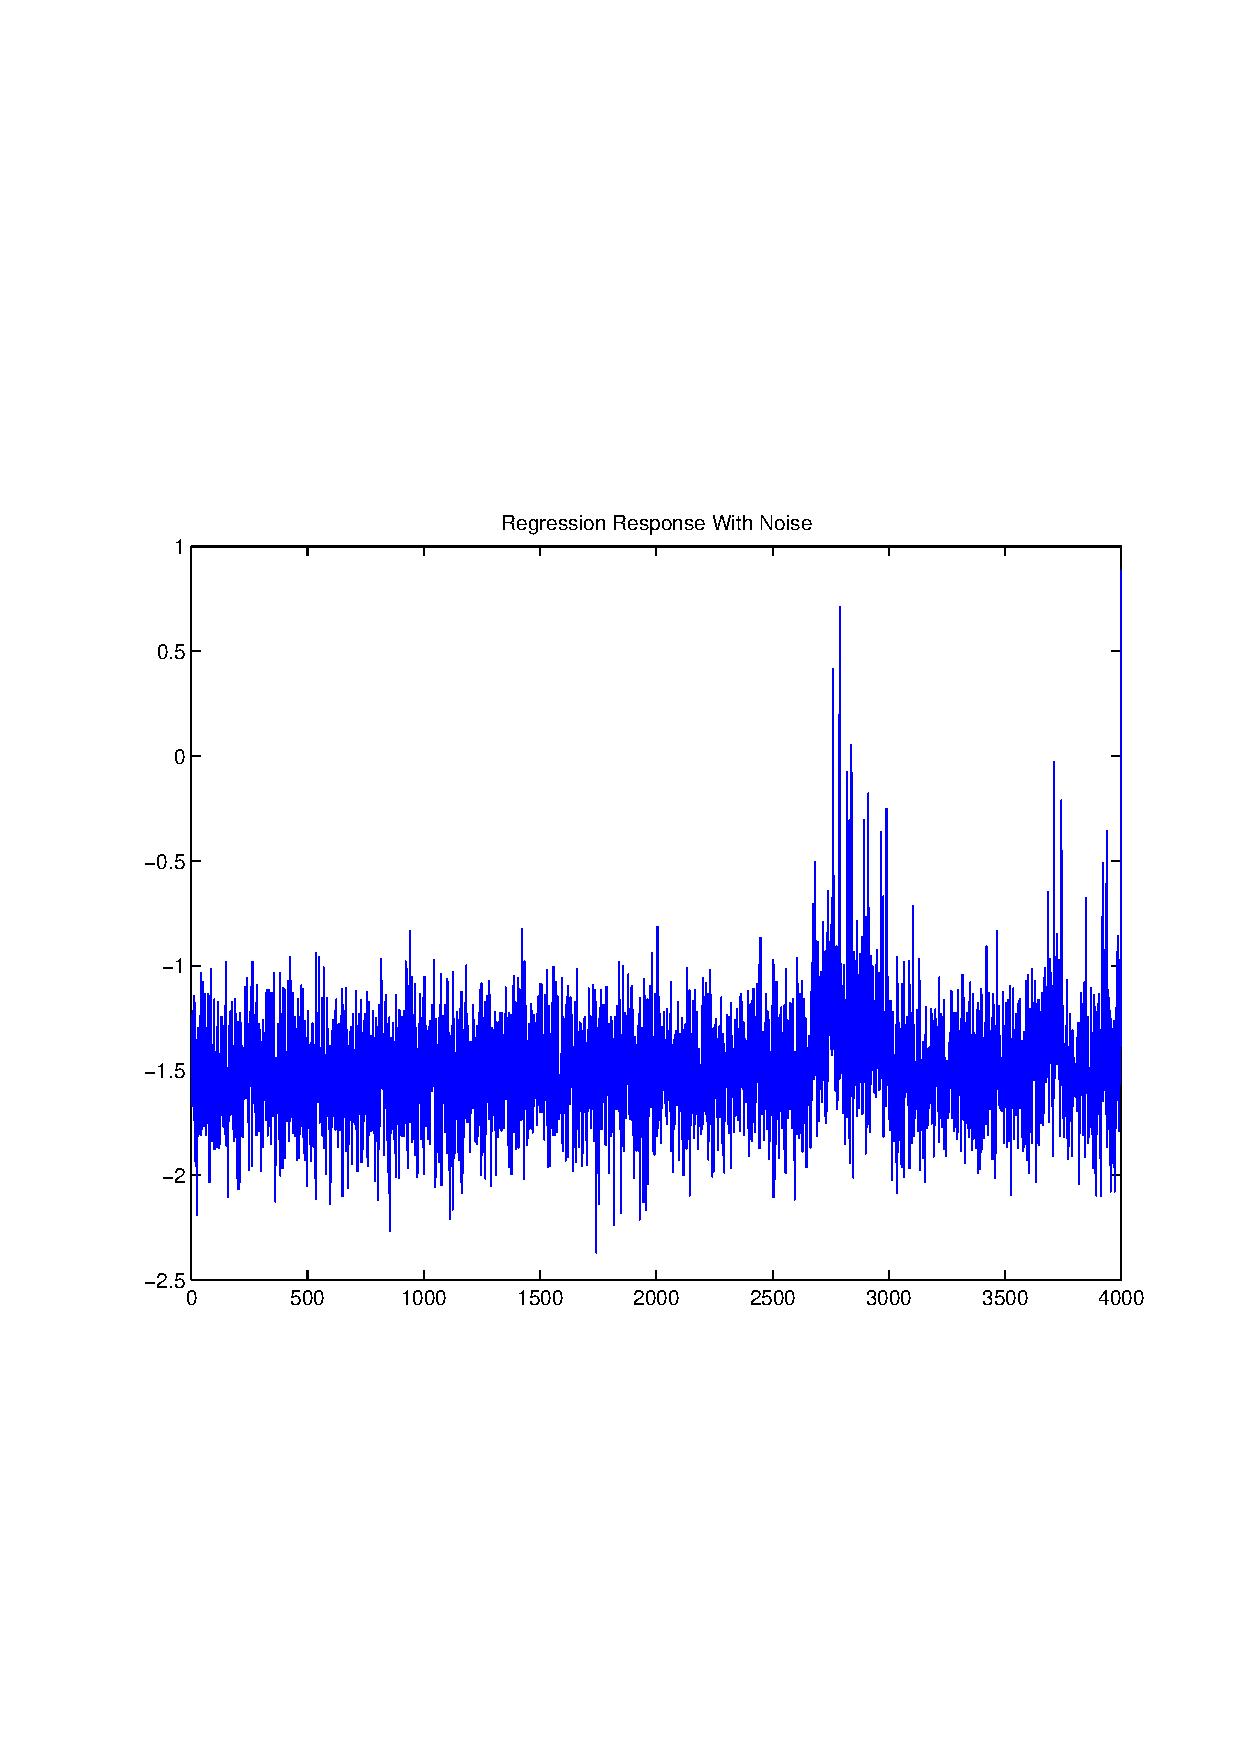
\includegraphics[width=10.0cm,height=10.0cm]{AtanDataSet_regression_response_with_noise.pdf}

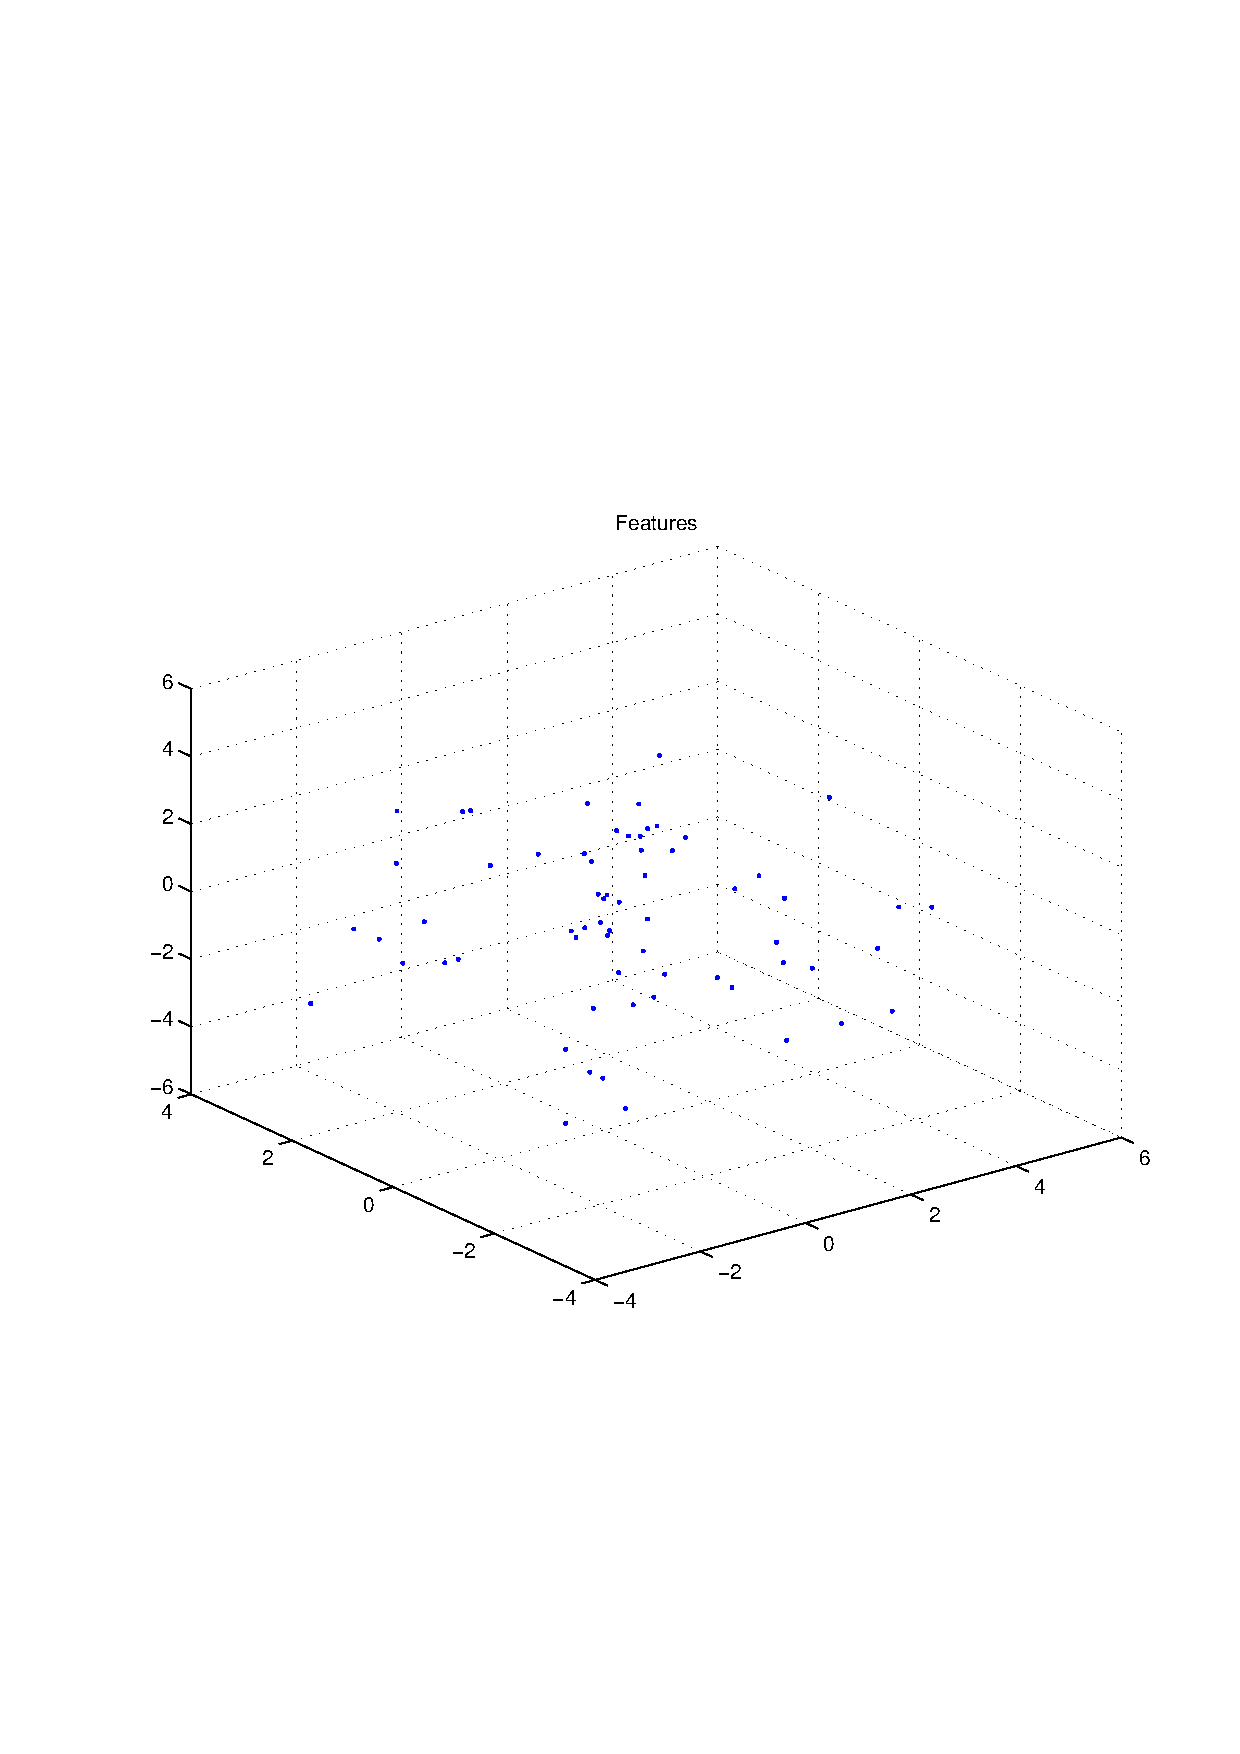
\includegraphics[width=10.0cm,height=10.0cm]{regression_features.pdf}

Response
-1.438
-1.668
-1.583
-1.237
-1.310
-1.349
-1.413
-1.282
-1.310
-1.144
-1.668
-1.382
-1.735
-1.506
-1.433
-1.933
-1.179
-1.378
-1.955
-1.596
-1.428
-1.537
-1.355
-1.862
-1.479
-2.192
-1.299
-1.390
-1.460
-1.773
-1.595
-1.361
-1.805
-1.779
-1.687
-1.240
-1.251
-1.506
-1.352
-1.810
-1.170
-1.378
-1.036
-1.262
-1.231
-1.778
-1.526
-1.694
-1.512
-1.076
-1.407
-1.278
-1.561
-1.765
-1.441
-1.673
-1.457
-1.137
-1.676
-1.674
-1.495
-1.775
-1.536
-1.644
-1.807
-1.300
-1.491
-1.716
-1.532
-1.499
-1.183
-1.135
-1.752
-1.240
-1.673
-1.847
-1.612
-2.034
-1.147
-1.594
-1.437
-1.529
-1.651
-1.035
-1.347
-1.017
-1.654
-1.508
-1.838
-1.552
-1.529
-1.384
-1.379
-1.526
-1.408
-1.585
-1.388
-1.236
-1.161
-1.875
-1.832
-1.535
-1.613
-1.842
-1.699
-1.832
-1.410
-1.487
-1.608
-1.631
-1.867
-1.446
-1.172
-1.376
-1.760
-1.617
-1.812
-1.421
-1.872
-1.558
-1.675
-1.626
-1.853
-1.729
-1.799
-1.564
-1.713
-1.459
-1.409
-1.245
-1.683
-1.615
-1.707
-1.666
-1.552
-1.515
-1.581
-1.768
-1.712
-1.414
-1.664
-1.463
-1.286
-1.766
-1.804
-1.191
-1.736
-0.984
-1.625
-1.779
-1.858
-1.542
-1.488
-1.740
-1.570
-1.638
-1.679
-1.489
-2.106
-1.712
-1.379
-1.308
-1.286
-1.427
-1.681
-1.596
-1.339
-1.218
-1.711
-1.500
-1.386
-1.483
-1.374
-1.184
-1.175
-1.531
-1.631
-1.780
-1.496
-1.384
-1.492
-1.591
-1.839
-1.598
-1.482
-1.821
-1.159
-1.227
-1.567
-1.446
-1.759
-1.231
-1.730
-1.390
-1.479
-1.423
-2.015
-1.416
-1.552
-1.628
-1.269
-1.363
-2.068
-1.750
-1.346
-1.399
-2.032
-1.398
-1.465
-1.225
-1.550
-1.275
-1.617
-1.740
-1.275
-1.389
-1.517
-1.814
-1.732
-1.528
-1.818
-1.438
-1.618
-1.502
-1.445
-1.395
-1.635
-1.545
-1.541
-1.104
-1.442
-1.379
-1.393
-1.171
-1.622
-1.634
-1.521
-1.437
-1.399
-1.057
-1.482
-1.535
-1.645
-1.628
-1.321
-1.746
-1.281
-1.453
-1.976
-1.525
-1.510
-1.428
-1.424
-1.362
-1.105
-1.543
-1.334
-1.577
-1.340
-1.957
-1.941
-1.483
-0.981
-1.324
-1.656
-1.195
-1.377
-1.233
-1.566
-1.638
-1.499
-1.260
-1.631
-1.438
-1.701
-1.454
-1.192
-1.748
-1.177
-1.807
-1.346
-1.456
-1.094
-1.808
-1.637
-1.595
-1.714
-1.548
-1.500
-1.362
-1.280
-1.790
-1.441
-1.308
-1.573
-1.516
-1.423
-1.491
-1.981
-1.964
-1.365
-1.451
-1.586
-1.540
-1.681
-1.610
-1.262
-1.867
-1.456
-1.748
-1.319
-1.435
-1.641
-1.325
-1.534
-1.560
-1.579
-1.509
-1.410
-1.130
-1.508
-1.524
-1.735
-1.403
-1.117
-1.588
-1.581
-1.811
-1.395
-1.607
-1.593
-1.417
-1.414
-1.560
-1.115
-1.654
-1.412
-1.208
-1.763
-1.287
-1.414
-1.185
-1.853
-1.314
-1.129
-1.635
-1.649
-1.711
-1.408
-1.433
-1.717
-1.371
-1.468
-1.255
-1.034
-1.094
-1.609
-1.482
-1.562
-1.499
-2.126
-1.439
-1.953
-1.520
-1.459
-1.671
-1.474
-1.624
-1.612
-1.693
-1.279
-1.502
-1.518
-1.704
-1.562
-1.464
-1.585
-1.732
-1.830
-1.036
-1.853
-1.370
-2.002
-1.797
-1.594
-1.621
-1.233
-1.720
-1.244
-1.359
-1.373
-1.967
-1.774
-1.110
-1.698
-1.286
-1.616
-1.877
-1.608
-1.375
-1.114
-1.612
-1.573
-1.919
-1.678
-1.548
-1.667
-1.546
-1.587
-1.488
-1.743
-1.413
-1.499
-1.452
-1.615
-1.297
-1.072
-1.333
-1.317
-1.520
-1.503
-1.838
-1.617
-1.250
-0.961
-1.590
-1.072
-1.720
-1.268
-1.440
-1.422
-1.198
-1.168
-1.381
-1.130
-1.561
-1.798
-1.692
-1.493
-1.395
-1.573
-1.603
-1.686
-1.315
-1.247
-1.394
-1.812
-1.301
-1.317
-1.461
-1.390
-1.318
-1.834
-1.641
-1.509
-1.929
-1.158
-1.232
-1.346
-1.630
-1.890
-1.555
-1.920
-1.772
-1.244
-1.755
-1.803
-1.537
-1.544
-1.199
-1.422
-1.653
-1.095
-1.163
-1.675
-1.765
-1.397
-1.112
-1.530
-1.787
-1.235
-1.724
-1.896
-1.336
-1.725
-1.512
-1.403
-1.266
-1.928
-1.468
-1.626
-1.527
-1.497
-1.521
-1.365
-1.427
-2.051
-1.344
-1.798
-1.602
-1.215
-1.280
-1.733
-1.500
-1.773
-1.582
-1.377
-1.514
-1.852
-1.408
-1.557
-1.513
-1.826
-1.629
-1.370
-1.932
-1.773
-1.529
-1.370
-1.418
-1.275
-1.799
-1.486
-1.751
-1.863
-1.761
-1.851
-1.465
-1.380
-1.502
-1.378
-2.014
-1.403
-1.499
-0.935
-1.560
-2.115
-1.343
-1.395
-1.225
-1.435
-1.300
-1.430
-1.653
-1.486
-1.450
-1.535
-1.415
-1.471
-0.960
-1.322
-1.731
-1.749
-1.538
-1.638
-1.478
-1.628
-1.393
-1.427
-1.458
-1.452
-1.156
-1.811
-1.548
-1.725
-1.450
-1.495
-1.616
-1.009
-1.554
-1.629
-1.502
-1.871
-1.674
-1.426
-1.835
-1.552
-1.565
-1.699
-1.639
-1.996
-1.347
-1.156
-1.698
-1.503
-1.542
-1.661
-1.392
-1.305
-1.468
-1.416
-1.778
-1.491
-1.584
-1.504
-1.384
-1.845
-2.136
-1.895
-1.535
-1.721
-1.523
-1.405
-1.725
-1.769
-1.313
-1.341
-1.615
-1.719
-1.260
-1.656
-1.660
-1.415
-1.424
-1.657
-1.301
-1.218
-1.500
-1.464
-1.782
-1.188
-1.268
-1.162
-1.189
-1.520
-1.346
-1.356
-1.535
-1.319
-1.867
-1.734
-1.648
-1.284
-1.683
-1.278
-1.290
-1.460
-1.784
-1.442
-1.353
-1.780
-1.277
-1.239
-1.303
-1.517
-1.753
-1.735
-1.111
-2.098
-1.278
-1.529
-1.636
-1.189
-2.099
-1.217
-1.546
-1.424
-1.572
-1.692
-1.595
-1.438
-1.710
-1.392
-1.885
-1.108
-1.290
-1.733
-1.307
-1.315
-1.633
-1.704
-1.676
-1.445
-1.765
-2.062
-1.578
-1.818
-1.850
-1.766
-1.383
-1.632
-1.660
-1.496
-1.317
-1.465
-1.422
-1.344
-1.295
-1.737
-1.487
-1.362
-1.308
-1.949
-1.230
-1.502
-1.667
-1.440
-1.727
-1.744
-1.726
-1.405
-1.566
-1.755
-1.631
-1.419
-1.401
-1.487
-1.122
-1.779
-1.416
-1.644
-1.588
-1.717
-1.400
-1.981
-1.840
-1.401
-1.674
-1.288
-1.708
-1.496
-1.310
-1.230
-1.477
-1.514
-1.414
-1.607
-1.716
-1.285
-1.559
-1.165
-1.937
-1.522
-1.424
-1.324
-1.530
-1.533
-1.594
-1.713
-1.877
-1.333
-1.743
-1.502
-1.435
-1.264
-1.569
-1.498
-1.230
-1.458
-1.405
-1.230
-1.551
-1.442
-1.915
-1.305
-1.125
-1.525
-1.849
-1.510
-1.956
-1.317
-1.645
-1.436
-1.806
-1.172
-1.648
-1.761
-1.454
-1.535
-1.660
-1.335
-1.691
-1.788
-1.526
-1.679
-1.694
-1.745
-1.429
-1.747
-1.217
-1.322
-1.785
-1.581
-1.346
-1.797
-1.499
-1.565
-1.530
-2.027
-1.463
-1.649
-1.756
-1.646
-1.713
-1.253
-1.743
-1.521
-1.291
-1.458
-1.839
-1.414
-1.802
-2.116
-1.878
-1.409
-1.644
-1.374
-1.874
-1.187
-1.200
-1.297
-1.765
-1.586
-1.583
-0.970
-1.501
-1.337
-1.394
-1.552
-1.332
-1.072
-1.505
-1.529
-1.390
-1.470
-1.328
-1.796
-1.513
-1.558
-1.905
-1.509
-1.455
-1.175
-1.470
-1.465
-1.496
-1.139
-1.300
-1.495
-1.832
-1.450
-1.280
-1.637
-1.629
-1.986
-1.322
-1.499
-1.544
-2.083
-1.589
-1.817
-1.248
-1.627
-1.597
-2.267
-1.740
-1.798
-1.431
-1.346
-1.644
-1.532
-1.755
-1.781
-1.598
-1.476
-1.305
-1.696
-1.277
-1.660
-1.828
-1.539
-1.458
-1.683
-1.365
-1.676
-1.892
-1.686
-1.512
-1.803
-1.543
-2.007
-1.140
-1.507
-1.754
-1.344
-1.421
-1.638
-1.677
-1.652
-1.323
-1.508
-1.267
-1.560
-1.211
-2.014
-1.430
-1.463
-1.219
-1.687
-1.287
-1.809
-1.633
-1.282
-1.290
-1.814
-1.796
-1.247
-1.608
-1.596
-1.380
-1.751
-1.470
-1.296
-1.217
-1.813
-1.485
-1.547
-1.487
-1.749
-1.718
-1.392
-0.980
-1.605
-1.243
-1.575
-1.439
-1.017
-1.703
-1.880
-1.709
-1.970
-1.781
-1.754
-1.602
-1.308
-1.468
-1.097
-1.415
-1.417
-1.719
-0.837
-1.747
-1.378
-1.423
-1.557
-1.554
-1.054
-1.605
-1.518
-1.465
-1.840
-1.509
-1.396
-1.238
-1.348
-1.289
-1.829
-1.683
-1.467
-1.562
-1.903
-1.090
-1.597
-1.297
-1.683
-1.340
-1.792
-1.315
-1.689
-1.398
-2.009
-1.825
-1.600
-1.729
-1.475
-1.987
-1.562
-1.658
-1.343
-1.501
-1.276
-1.449
-1.567
-1.524
-1.137
-1.268
-1.829
-1.578
-1.484
-1.438
-1.449
-1.568
-1.348
-1.390
-1.866
-1.357
-1.601
-1.204
-1.110
-1.580
-1.994
-1.670
-1.053
-1.743
-1.610
-1.605
-1.285
-1.412
-1.767
-1.342
-1.601
-1.559
-1.348
-1.484
-1.324
-1.312
-1.826
-1.465
-1.555
-1.321
-1.294
-1.690
-1.340
-1.450
-1.559
-1.563
-1.850
-1.263
-1.543
-1.467
-1.528
-1.476
-1.400
-1.599
-1.191
-1.593
-1.257
-1.462
-1.235
-1.288
-1.516
-1.479
-1.570
-0.971
-1.576
-1.531
-1.628
-1.421
-2.058
-1.601
-1.804
-1.257
-1.448
-2.008
-1.727
-1.656
-1.731
-1.434
-1.558
-1.557
-1.379
-1.416
-1.488
-1.605
-1.935
-1.335
-1.248
-1.579
-1.395
-1.283
-1.316
-1.184
-1.705
-1.390
-1.042
-2.049
-1.837
-1.529
-1.411
-1.499
-1.500
-1.654
-1.243
-1.477
-1.613
-1.654
-1.597
-1.365
-1.383
-1.453
-1.186
-1.793
-1.500
-1.459
-1.606
-1.344
-1.285
-1.355
-1.774
-1.066
-1.894
-1.347
-1.332
-1.808
-1.079
-1.789
-1.372
-1.976
-1.537
-1.322
-2.210
-1.746
-1.544
-1.504
-1.783
-1.341
-1.334
-1.897
-1.567
-1.848
-1.551
-1.290
-1.694
-2.164
-1.031
-1.579
-1.063
-1.515
-1.800
-1.600
-1.918
-1.616
-1.498
-1.892
-1.491
-1.633
-1.418
-1.566
-1.571
-1.731
-1.372
-1.222
-1.339
-1.500
-1.656
-1.262
-1.507
-1.891
-1.384
-1.494
-1.926
-1.521
-1.352
-1.800
-1.209
-1.623
-1.650
-1.316
-1.240
-2.031
-1.769
-1.124
-1.739
-1.951
-1.753
-2.087
-1.862
-1.327
-1.599
-1.569
-1.310
-1.820
-1.478
-1.353
-1.731
-1.500
-1.180
-1.600
-1.246
-1.379
-1.598
-1.224
-0.999
-1.546
-1.329
-1.424
-1.568
-1.748
-1.536
-1.289
-1.359
-1.444
-1.626
-1.611
-1.555
-1.370
-1.728
-1.711
-1.724
-1.890
-1.363
-1.479
-1.705
-1.465
-1.452
-1.524
-1.481
-1.554
-1.519
-1.470
-1.678
-1.326
-1.186
-1.356
-1.374
-1.380
-1.611
-1.345
-1.476
-1.700
-1.652
-1.839
-1.490
-1.588
-1.771
-1.715
-1.293
-1.852
-1.290
-1.384
-1.815
-1.508
-1.450
-1.459
-1.687
-1.227
-1.523
-1.362
-1.318
-1.761
-1.176
-1.310
-1.116
-1.364
-2.001
-1.407
-1.492
-1.085
-1.539
-1.484
-1.785
-1.903
-1.632
-1.623
-1.691
-1.354
-1.261
-1.670
-1.250
-1.890
-1.673
-1.175
-1.681
-1.901
-2.016
-1.512
-1.174
-1.217
-1.462
-1.462
-1.144
-1.620
-1.652
-1.651
-1.368
-1.597
-1.597
-1.653
-1.495
-1.718
-1.073
-1.731
-1.436
-1.139
-1.330
-1.706
-1.665
-2.050
-1.482
-1.359
-1.741
-1.296
-1.402
-1.543
-1.788
-1.599
-1.557
-1.714
-1.371
-1.711
-1.530
-1.308
-1.631
-1.528
-1.613
-1.649
-1.787
-1.221
-2.000
-1.604
-1.269
-1.371
-1.515
-1.276
-1.496
-1.291
-1.463
-1.816
-1.404
-1.710
-1.722
-1.286
-1.267
-1.774
-1.754
-1.225
-1.537
-1.708
-1.677
-1.684
-1.511
-1.452
-1.787
-1.225
-1.767
-1.786
-1.545
-1.478
-1.387
-1.381
-1.640
-1.546
-1.662
-1.775
-1.416
-1.330
-1.416
-1.598
-1.255
-1.230
-1.483
-1.104
-1.633
-1.378
-1.637
-1.357
-1.381
-1.283
-1.328
-1.248
-1.514
-1.662
-1.359
-1.843
-1.962
-1.225
-1.828
-1.682
-1.524
-1.616
-1.847
-1.461
-1.532
-1.236
-1.313
-1.350
-1.995
-1.696
-1.408
-1.529
-1.626
-1.096
-1.504
-1.301
-1.537
-1.336
-1.794
-1.050
-1.168
-1.170
-1.645
-1.567
-1.545
-1.319
-1.876
-1.333
-1.333
-1.630
-1.180
-1.817
-1.206
-1.411
-1.569
-1.580
-1.061
-1.805
-1.868
-1.242
-1.668
-1.383
-1.110
-1.486
-1.356
-1.118
-1.571
-1.418
-1.736
-1.158
-1.558
-1.551
-1.360
-1.460
-1.314
-0.827
-1.323
-1.562
-1.643
-1.519
-1.734
-1.227
-2.019
-1.505
-0.980
-1.363
-1.416
-1.384
-1.683
-1.534
-1.196
-1.601
-1.377
-1.857
-1.392
-1.359
-1.442
-1.478
-1.822
-1.360
-1.747
-1.728
-1.464
-1.781
-1.278
-1.596
-1.489
-1.417
-1.639
-1.776
-1.497
-1.184
-1.691
-1.514
-1.214
-1.780
-1.463
-1.445
-1.670
-1.797
-1.337
-1.306
-1.626
-1.234
-1.630
-1.672
-1.578
-1.270
-1.455
-1.633
-1.277
-1.507
-1.294
-1.283
-1.534
-1.426
-1.762
-1.403
-1.336
-1.229
-1.508
-1.497
-1.307
-1.547
-1.148
-1.344
-1.660
-1.668
-1.274
-1.550
-1.589
-1.698
-1.391
-1.087
-1.505
-1.172
-1.212
-1.598
-1.094
-1.535
-1.696
-1.259
-1.422
-1.659
-1.629
-1.538
-1.379
-1.465
-1.543
-1.830
-1.543
-1.505
-1.143
-1.355
-1.172
-1.643
-1.640
-1.585
-1.410
-1.021
-1.409
-1.503
-1.759
-1.424
-1.962
-1.374
-1.346
-1.829
-1.556
-1.193
-1.640
-1.703
-1.324
-1.537
-1.408
-1.955
-1.358
-1.618
-1.510
-1.371
-1.774
-1.347
-1.180
-1.650
-1.178
-1.420
-1.185
-1.413
-1.808
-1.005
-1.753
-1.481
-1.569
-1.582
-1.807
-1.757
-1.092
-1.265
-1.315
-1.077
-1.406
-1.479
-1.796
-1.455
-1.571
-1.640
-1.621
-1.148
-1.321
-1.288
-1.521
-1.632
-1.732
-1.697
-1.543
-1.524
-1.667
-1.692
-1.654
-1.539
-1.436
-1.477
-1.705
-1.422
-1.844
-1.062
-1.352
-1.802
-1.593
-1.244
-1.884
-1.516
-1.703
-1.374
-1.643
-1.587
-1.331
-1.550
-1.678
-1.589
-1.253
-1.931
-1.190
-1.383
-1.586
-1.441
-1.710
-1.716
-1.151
-1.472
-1.487
-1.267
-1.913
-1.097
-1.453
-1.621
-1.621
-1.451
-1.661
-1.514
-1.575
-1.492
-1.152
-1.482
-1.497
-1.201
-1.580
-1.234
-1.349
-1.355
-1.298
-1.504
-1.982
-1.752
-1.567
-1.482
-1.445
-1.640
-1.834
-1.866
-1.523
-1.601
-1.381
-1.174
-1.609
-1.429
-1.936
-1.560
-1.775
-1.605
-1.719
-1.018
-1.384
-1.402
-1.778
-1.406
-1.678
-1.866
-1.316
-1.731
-1.736
-1.271
-1.692
-1.277
-1.281
-1.614
-1.440
-1.281
-1.486
-1.666
-1.459
-1.957
-1.628
-1.311
-1.497
-1.894
-1.742
-1.490
-1.532
-1.256
-1.589
-1.344
-1.304
-1.648
-1.697
-1.247
-1.304
-1.773
-1.717
-1.756
-1.685
-1.952
-1.443
-1.524
-1.579
-1.369
-1.695
-1.625
-1.641
-1.556
-1.108
-1.372
-1.512
-1.573
-1.472
-1.239
-1.681
-1.271
-1.575
-1.245
-1.773
-1.338
-1.279
-1.343
-1.328
-1.277
-1.686
-1.176
-1.471
-1.095
-1.556
-1.313
-1.217
-1.837
-1.676
-1.659
-1.116
-1.579
-1.442
-1.616
-1.552
-1.172
-1.963
-2.370
-1.299
-1.455
-1.766
-1.988
-1.643
-1.533
-1.547
-1.737
-1.660
-1.705
-2.140
-2.007
-1.316
-1.203
-1.544
-1.494
-1.431
-1.779
-1.367
-1.115
-1.635
-1.424
-1.690
-1.747
-1.627
-1.780
-1.349
-1.620
-1.465
-1.234
-1.187
-1.195
-1.360
-1.379
-1.653
-1.572
-1.301
-1.437
-1.853
-1.596
-1.857
-1.428
-1.185
-1.103
-1.451
-1.437
-1.527
-1.419
-1.617
-1.526
-1.369
-1.453
-1.368
-1.278
-1.988
-1.315
-1.743
-1.596
-1.664
-1.477
-1.578
-1.577
-1.812
-1.244
-1.533
-1.482
-1.380
-1.792
-1.263
-1.525
-1.441
-1.654
-1.789
-1.350
-1.636
-1.873
-2.240
-1.454
-1.540
-1.350
-1.650
-1.245
-1.344
-1.682
-1.568
-1.426
-1.657
-1.194
-1.411
-1.255
-1.659
-1.628
-1.523
-1.567
-1.684
-0.981
-1.695
-1.697
-1.275
-1.161
-1.484
-1.777
-1.679
-1.707
-1.580
-2.181
-1.335
-1.332
-1.828
-1.708
-1.490
-1.414
-1.571
-1.003
-1.862
-1.539
-1.263
-1.451
-1.883
-1.731
-1.309
-1.226
-1.544
-1.412
-1.484
-1.659
-1.285
-1.428
-1.729
-1.536
-1.359
-1.243
-1.296
-1.250
-1.502
-1.462
-1.306
-1.042
-1.589
-1.430
-1.708
-1.206
-1.518
-1.370
-1.730
-1.561
-1.494
-1.109
-1.339
-1.641
-1.435
-1.738
-1.330
-1.467
-1.098
-1.806
-1.510
-1.213
-1.233
-1.726
-1.777
-1.830
-2.015
-1.579
-1.486
-1.414
-1.618
-1.341
-1.472
-1.855
-1.378
-1.647
-1.883
-1.423
-1.624
-1.653
-1.617
-1.290
-1.341
-1.694
-1.353
-1.232
-1.385
-1.693
-1.887
-1.570
-2.212
-1.154
-1.606
-1.484
-1.717
-1.395
-1.553
-1.626
-1.360
-1.300
-1.816
-1.463
-1.698
-1.623
-1.667
-1.512
-2.129
-1.465
-1.344
-1.065
-1.322
-1.272
-1.287
-1.143
-1.376
-1.619
-1.395
-1.433
-2.166
-1.827
-1.624
-1.260
-1.282
-1.162
-2.044
-1.622
-1.240
-1.730
-1.706
-1.634
-1.270
-1.310
-1.097
-1.408
-1.512
-1.312
-1.373
-1.503
-1.675
-1.383
-1.560
-1.469
-0.938
-1.592
-1.286
-1.758
-1.415
-1.731
-1.884
-1.746
-1.491
-1.386
-1.338
-1.903
-1.304
-1.311
-1.441
-1.135
-1.454
-1.453
-1.179
-1.694
-1.291
-1.815
-1.759
-1.569
-0.815
-1.515
-0.914
-1.542
-1.775
-1.374
-1.542
-1.676
-1.150
-1.336
-1.402
-1.406
-1.737
-1.339
-1.294
-1.683
-1.658
-1.847
-1.452
-1.638
-1.544
-1.484
-1.543
-1.449
-1.295
-1.592
-1.463
-1.224
-1.585
-1.441
-1.354
-1.525
-1.560
-1.656
-1.372
-1.395
-1.453
-1.719
-1.639
-1.686
-1.758
-1.297
-1.209
-1.512
-1.437
-1.458
-1.639
-1.431
-1.314
-1.605
-1.434
-1.548
-1.443
-1.615
-1.626
-1.229
-1.696
-1.080
-1.411
-1.887
-1.432
-1.747
-1.731
-1.809
-1.497
-1.380
-1.550
-1.984
-1.417
-1.784
-1.705
-1.357
-1.540
-1.373
-1.758
-1.538
-1.555
-1.351
-1.310
-1.557
-1.510
-1.573
-1.666
-1.387
-1.418
-1.442
-1.395
-1.172
-1.300
-1.257
-1.330
-1.928
-1.783
-1.805
-1.368
-1.487
-1.366
-1.602
-1.327
-1.505
-1.372
-1.692
-1.564
-1.557
-1.501
-1.825
-1.817
-1.249
-1.630
-1.684
-1.513
-1.805
-2.001
-1.306
-1.660
-1.315
-1.587
-1.427
-1.757
-1.524
-1.281
-1.650
-1.296
-1.365
-1.311
-1.873
-1.011
-1.478
-1.318
-1.468
-1.356
-1.234
-1.473
-1.501
-1.365
-1.826
-1.639
-1.531
-1.118
-2.097
-1.696
-1.432
-1.540
-1.634
-1.672
-1.419
-1.760
-1.636
-1.439
-1.463
-1.325
-1.484
-1.396
-1.485
-1.168
-1.455
-1.541
-1.823
-1.473
-1.182
-1.758
-1.119
-1.277
-1.717
-1.674
-1.366
-1.228
-1.309
-1.222
-1.658
-1.709
-1.282
-1.514
-1.430
-1.601
-1.433
-1.876
-1.577
-1.423
-1.706
-1.399
-1.548
-1.606
-1.765
-1.475
-1.499
-1.691
-1.686
-1.804
-1.670
-1.408
-1.553
-1.194
-1.778
-1.278
-1.058
-1.755
-1.457
-1.696
-1.408
-1.419
-1.403
-1.436
-1.640
-1.557
-1.549
-1.151
-1.519
-1.221
-1.082
-1.707
-1.570
-1.498
-1.745
-1.648
-1.466
-1.362
-1.695
-1.138
-1.926
-1.722
-1.607
-1.433
-1.454
-1.419
-1.020
-1.618
-1.291
-1.648
-1.459
-1.139
-1.754
-1.672
-1.790
-1.305
-1.623
-2.007
-1.680
-1.379
-1.348
-1.347
-1.982
-1.388
-1.334
-1.297
-1.318
-1.282
-1.510
-1.522
-1.467
-1.256
-1.300
-1.630
-1.360
-1.351
-1.692
-1.626
-1.723
-1.691
-1.878
-1.469
-1.751
-1.702
-1.361
-1.547
-1.531
-1.291
-1.555
-1.640
-1.720
-1.582
-1.347
-1.500
-1.411
-1.500
-1.153
-1.730
-1.761
-1.779
-1.849
-1.637
-1.325
-1.594
-1.599
-1.905
-1.376
-1.715
-1.815
-1.988
-1.417
-1.527
-1.529
-1.537
-1.503
-1.581
-1.515
-1.447
-1.535
-1.330
-1.237
-1.246
-1.260
-1.757
-1.253
-1.493
-1.393
-1.798
-1.246
-1.338
-1.760
-1.537
-1.591
-1.523
-1.321
-1.368
-1.438
-1.483
-1.967
-1.177
-1.543
-1.525
-1.376
-1.576
-1.528
-1.433
-1.460
-1.589
-1.631
-1.399
-1.402
-1.792
-1.778
-1.490
-1.259
-1.445
-1.718
-1.468
-1.673
-1.386
-1.384
-1.577
-1.713
-1.513
-1.207
-1.310
-1.738
-1.436
-1.344
-1.674
-1.547
-1.395
-1.317
-1.535
-1.399
-1.790
-1.649
-1.684
-1.148
-1.367
-1.138
-1.381
-1.579
-1.174
-1.267
-1.516
-1.282
-1.588
-1.346
-1.484
-1.526
-1.271
-1.565
-1.397
-1.385
-1.807
-1.398
-1.351
-1.486
-1.517
-1.414
-1.361
-1.486
-1.574
-1.652
-1.555
-1.414
-1.544
-1.539
-1.773
-1.522
-1.539
-1.119
-1.278
-1.532
-1.911
-1.677
-1.419
-1.535
-1.494
-1.326
-1.581
-1.449
-1.183
-1.829
-1.288
-1.636
-1.835
-1.171
-1.327
-1.114
-1.362
-1.277
-1.329
-1.748
-1.376
-1.675
-1.434
-1.110
-1.623
-1.795
-1.464
-1.504
-1.288
-1.464
-1.457
-1.653
-1.246
-1.547
-1.470
-1.086
-1.484
-1.234
-1.378
-1.555
-1.383
-1.672
-1.479
-1.618
-0.998
-1.870
-1.559
-1.674
-1.355
-0.869
-1.266
-1.574
-1.645
-1.354
-1.689
-1.590
-1.709
-1.523
-1.450
-1.317
-1.652
-1.399
-1.519
-1.831
-1.577
-1.554
-1.707
-1.657
-1.372
-1.666
-1.273
-1.611
-1.135
-1.497
-1.419
-1.447
-1.778
-1.575
-1.546
-1.219
-1.512
-1.488
-1.586
-1.447
-1.667
-1.663
-1.261
-1.924
-1.545
-1.505
-1.541
-1.838
-1.631
-1.676
-1.649
-1.413
-1.628
-1.437
-1.712
-1.518
-1.192
-1.615
-0.972
-1.708
-1.751
-2.104
-1.566
-0.997
-1.483
-1.439
-1.710
-1.695
-2.016
-1.208
-1.701
-1.851
-1.741
-1.613
-1.077
-1.271
-1.131
-1.592
-1.712
-1.725
-1.251
-1.348
-1.631
-1.816
-1.916
-1.705
-1.475
-1.474
-1.238
-1.450
-1.451
-1.667
-1.695
-1.220
-1.291
-1.199
-1.552
-1.775
-1.322
-1.323
-1.465
-1.387
-1.555
-1.678
-1.395
-1.585
-1.246
-1.874
-1.191
-1.258
-1.556
-1.472
-1.982
-1.990
-1.018
-1.081
-1.608
-1.428
-1.608
-1.575
-1.365
-1.729
-1.261
-1.330
-1.398
-1.487
-1.679
-1.311
-1.607
-1.523
-1.310
-1.289
-1.684
-1.179
-1.386
-1.232
-1.481
-1.183
-1.458
-1.425
-1.643
-1.773
-1.667
-1.446
-1.434
-1.160
-1.481
-1.425
-1.654
-1.686
-1.819
-1.694
-2.116
-1.412
-1.650
-1.833
-1.503
-1.486
-1.663
-1.643
-1.436
-1.464
-0.965
-1.802
-1.790
-1.789
-1.088
-1.768
-1.216
-1.310
-1.823
-1.479
-1.488
-1.216
-1.264
-1.135
-1.578
-1.421
-1.800
-1.653
-1.325
-1.388
-1.446
-1.203
-1.073
-1.248
-1.888
-1.474
-1.497
-1.448
-1.256
-1.705
-1.720
-1.162
-1.486
-1.378
-1.752
-1.248
-1.437
-1.518
-1.261
-1.732
-1.254
-1.961
-1.404
-1.423
-1.395
-1.455
-1.651
-1.624
-1.548
-1.663
-1.350
-1.433
-1.455
-1.336
-1.568
-1.590
-1.395
-1.474
-1.868
-1.561
-1.174
-1.537
-1.294
-0.988
-1.643
-1.457
-1.485
-1.257
-1.401
-1.502
-1.383
-0.706
-0.952
-1.540
-1.415
-0.762
-0.993
-1.375
-1.131
-0.505
-1.393
-1.520
-1.139
-1.037
-1.397
-1.612
-1.582
-1.814
-1.346
-0.887
-1.017
-1.500
-1.547
-1.125
-1.740
-1.226
-1.581
-1.567
-1.352
-1.054
-1.348
-1.587
-1.253
-1.496
-1.032
-1.254
-1.308
-1.649
-1.229
-1.596
-1.461
-0.979
-0.794
-0.834
-1.318
-0.947
-1.336
-1.012
-1.327
-1.719
-1.142
-1.284
-0.932
-1.328
-1.262
-1.510
-1.753
-1.040
-1.276
-0.845
-1.434
-1.695
-1.357
-0.643
-1.187
-1.151
-1.334
-0.986
-1.032
-1.332
-0.886
-1.268
-0.953
-1.191
-1.164
-1.031
-1.167
-0.808
-1.372
-1.426
-1.048
-0.926
-0.677
-1.205
-1.268
-1.236
+0.416
-1.399
-1.175
-1.276
-0.575
-1.179
-1.061
-1.227
-0.919
-1.597
-1.504
-1.436
-1.547
-1.251
-0.909
-1.458
-1.476
-1.059
-1.684
-1.588
-1.450
-1.182
-1.412
-1.356
+0.197
-0.539
-1.115
-0.787
-1.539
+0.708
-1.349
-1.410
-1.514
-0.994
-1.196
-1.145
-1.463
-1.246
-1.312
-1.099
-1.198
-1.418
-1.395
-1.705
-1.475
-1.250
-1.479
-1.334
-0.997
-1.395
-1.252
-1.392
-1.853
-1.221
-1.286
-1.459
-1.554
-1.723
-1.239
-1.334
-0.076
-0.927
-1.609
-1.581
-1.443
-0.784
-1.141
-1.821
-1.260
-1.291
-0.307
-1.943
-1.587
-1.409
-1.419
-1.625
+0.054
-0.421
-1.134
-0.082
-1.155
-1.432
-1.535
-1.201
-1.633
-0.942
-2.011
-1.190
-0.933
-1.630
-1.532
-1.311
-1.558
-1.326
-1.103
-1.570
-1.388
-0.979
-1.349
-1.199
-1.354
-0.965
-0.789
-1.718
-1.054
-1.042
-1.581
-1.548
-1.616
-1.407
-1.681
-1.348
-1.548
-1.096
-1.348
-1.150
-1.553
-0.944
-1.082
-1.213
-0.944
-1.164
-1.707
-0.862
-1.060
-1.212
-1.414
-1.070
-1.206
-1.702
-1.538
-1.254
-0.306
-1.337
-1.553
-1.127
-1.384
-1.220
-1.555
-1.146
-1.897
-1.061
-0.769
-1.447
-1.261
-1.500
-1.677
-1.768
-1.750
-1.237
-1.232
-0.179
-1.469
-1.035
-1.330
-1.265
-1.388
-1.231
-1.148
-1.795
-1.520
-1.564
-0.953
-1.378
-1.032
-1.236
-1.466
-1.230
-1.498
-1.004
-1.243
-1.247
-1.465
-1.187
-1.202
-1.243
-1.252
-1.605
-1.197
-1.600
-1.170
-1.340
-1.261
-1.628
-1.049
-1.403
-0.995
-0.980
-0.925
-1.232
-1.077
-1.126
-1.406
-1.326
-1.488
-1.386
-1.315
-1.593
-1.035
-1.198
-1.346
-1.135
-1.586
-1.365
-0.791
-1.511
-1.464
-0.364
-1.345
-1.008
-0.748
-1.229
-1.535
-1.562
-1.585
-0.670
-1.816
-1.402
-1.525
-1.222
-1.370
-1.386
-1.321
-1.314
-1.492
-1.604
-1.228
-1.488
-1.670
-0.253
-1.336
-1.254
-1.412
-0.916
-1.569
-1.421
-1.055
-1.292
-1.365
-1.336
-1.458
-1.734
-1.593
-1.320
-1.784
-1.294
-1.169
-1.388
-1.652
-1.576
-1.209
-1.252
-1.404
-1.755
-2.021
-1.625
-1.623
-1.221
-1.545
-1.492
-1.506
-1.835
-1.731
-1.428
-1.606
-1.726
-1.553
-1.468
-1.479
-1.292
-1.516
-1.281
-1.938
-1.640
-0.960
-2.083
-1.568
-1.571
-1.089
-1.890
-1.610
-1.768
-1.336
-1.275
-1.590
-1.595
-1.830
-1.778
-1.517
-1.773
-1.320
-1.949
-1.555
-1.577
-1.086
-1.900
-1.960
-1.796
-1.673
-1.237
-1.806
-1.560
-1.193
-0.983
-2.009
-1.415
-1.868
-1.303
-1.518
-1.546
-1.291
-1.598
-1.605
-1.375
-1.540
-1.282
-1.281
-1.557
-1.244
-1.329
-1.355
-1.491
-1.665
-1.632
-1.661
-0.980
-1.468
-1.672
-1.968
-1.207
-1.091
-1.522
-1.580
-1.272
-1.447
-1.631
-1.507
-1.351
-1.226
-1.847
-1.790
-1.527
-0.714
-1.646
-1.786
-1.430
-1.559
-1.282
-1.816
-1.599
-1.584
-1.729
-1.523
-1.539
-1.535
-1.460
-1.644
-1.686
-1.544
-1.455
-1.212
-1.419
-1.615
-1.418
-1.572
-1.378
-1.790
-1.557
-1.393
-0.969
-1.480
-1.453
-1.233
-1.076
-1.645
-1.976
-1.515
-1.530
-1.553
-1.654
-1.741
-1.725
-1.522
-1.785
-1.448
-1.414
-1.367
-1.918
-1.541
-1.568
-1.681
-1.577
-1.519
-2.033
-1.331
-1.598
-1.644
-1.647
-1.570
-1.461
-1.199
-1.416
-1.776
-1.522
-1.587
-1.767
-1.760
-1.704
-1.583
-1.554
-1.413
-1.537
-1.680
-1.431
-1.391
-1.399
-1.531
-1.537
-1.587
-1.265
-1.400
-1.208
-1.538
-1.754
-1.235
-1.717
-1.232
-1.564
-1.600
-1.267
-1.710
-1.412
-1.912
-1.895
-1.688
-1.420
-1.763
-1.759
-1.417
-1.209
-1.258
-1.407
-1.348
-1.576
-1.330
-1.436
-1.293
-1.544
-1.505
-1.604
-1.440
-1.691
-1.643
-1.599
-1.842
-1.831
-1.057
-1.456
-1.657
-1.729
-1.249
-1.351
-1.406
-1.481
-1.232
-1.369
-1.442
-1.562
-1.417
-1.247
-1.771
-1.284
-1.559
-1.462
-1.353
-1.340
-1.873
-1.654
-1.163
-1.816
-1.648
-1.749
-1.596
-1.458
-1.799
-1.523
-1.907
-1.541
-1.574
-1.704
-1.455
-1.582
-1.717
-1.608
-1.504
-1.729
-1.666
-1.370
-1.421
-1.571
-1.502
-1.515
-1.399
-1.413
-1.571
-1.120
-1.582
-1.372
-1.470
-1.123
-1.541
-1.726
-1.397
-1.495
-1.643
-1.629
-1.406
-1.632
-1.225
-1.617
-1.788
-1.742
-1.760
-1.574
-1.771
-1.285
-1.630
-1.454
-1.228
-1.500
-1.318
-1.580
-1.827
-1.363
-1.451
-1.115
-1.793
-1.258
-1.188
-1.539
-1.340
-1.425
-1.491
-1.577
-1.435
-1.312
-1.620
-1.335
-1.512
-1.884
-1.534
-1.450
-1.105
-1.690
-1.565
-1.164
-1.045
-1.171
-1.661
-1.735
-1.634
-1.375
-1.578
-1.462
-1.153
-1.421
-1.528
-1.941
-1.783
-1.524
-1.302
-1.516
-1.518
-1.653
-1.320
-1.228
-1.253
-1.725
-1.773
-1.630
-1.505
-1.743
-1.258
-1.455
-1.816
-1.575
-1.174
-1.775
-1.464
-1.600
-1.081
-1.649
-1.689
-1.517
-1.672
-1.582
-1.879
-1.604
-1.500
-1.828
-1.589
-1.135
-1.489
-1.560
-1.472
-1.324
-1.756
-1.320
-1.406
-1.721
-1.822
-1.586
-1.486
-1.331
-1.488
-1.869
-1.525
-1.789
-1.210
-1.648
-1.624
-1.745
-1.256
-1.988
-1.177
-1.218
-1.541
-1.583
-1.687
-1.781
-1.556
-1.422
-1.972
-1.338
-1.736
-1.890
-1.652
-1.112
-1.815
-1.701
-1.875
-1.140
-1.371
-1.451
-1.630
-1.354
-1.461
-1.345
-1.822
-1.451
-1.673
-1.272
-1.550
-1.477
-1.510
-1.525
-1.293
-1.754
-0.992
-0.908
-1.022
-1.496
-1.149
-1.483
-1.810
-1.171
-1.339
-1.371
-1.307
-1.132
-1.458
-1.459
-1.685
-1.520
-1.361
-1.314
-1.609
-1.439
-1.525
-1.642
-1.416
-1.257
-1.598
-1.392
-1.249
-1.924
-1.136
-1.486
-1.251
-1.613
-1.250
-1.188
-1.525
-1.306
-1.379
-2.012
-1.351
-1.320
-1.636
-1.892
-1.562
-1.849
-1.324
-0.837
-1.537
-1.460
-1.315
-1.444
-1.281
-1.213
-1.588
-1.193
-1.394
-1.449
-1.582
-1.669
-1.678
-1.334
-1.355
-1.518
-1.656
-1.593
-1.555
-1.690
-1.693
-1.552
-1.442
-1.473
-1.600
-1.522
-1.406
-1.126
-1.310
-1.791
-1.290
-1.848
-1.356
-1.421
-1.435
-1.668
-1.320
-1.624
-1.508
-1.355
-1.178
-1.674
-1.310
-1.608
-1.868
-1.329
-1.404
-1.165
-1.675
-1.678
-1.758
-1.836
-1.451
-1.383
-1.481
-1.486
-1.095
-1.586
-1.456
-1.362
-1.353
-2.095
-1.527
-1.681
-1.449
-1.505
-1.614
-1.641
-1.636
-1.195
-1.506
-1.109
-1.829
-1.310
-1.464
-1.489
-1.320
-1.673
-1.451
-1.474
-1.371
-1.232
-1.431
-1.713
-1.714
-1.562
-1.599
-1.410
-1.436
-1.872
-1.182
-1.687
-1.493
-1.255
-1.492
-1.619
-1.170
-1.475
-1.431
-1.160
-1.440
-1.680
-1.480
-1.591
-1.469
-1.413
-1.815
-1.361
-1.645
-1.358
-1.688
-1.514
-1.629
-1.581
-1.887
-1.440
-1.319
-1.863
-1.578
-1.440
-1.601
-1.633
-1.852
-1.438
-1.851
-1.416
-1.544
-1.074
-1.761
-1.595
-1.929
-1.623
-1.269
-1.045
-1.707
-1.537
-1.577
-1.255
-1.345
-1.994
-1.781
-1.207
-1.546
-1.302
-1.360
-1.633
-1.655
-1.490
-1.648
-1.061
-1.015
-1.645
-1.846
-1.313
-1.392
-1.547
-1.430
-1.547
-1.462
-1.521
-1.413
-1.179
-1.358
-1.547
-1.072
-1.361
-1.502
-1.342
-1.631
-2.031
-1.183
-1.328
-1.677
-1.815
-1.456
-1.659
-1.647
-1.611
-1.847
-1.162
-1.858
-1.542
-1.790
-1.221
-1.326
-1.593
-1.355
-1.552
-1.751
-1.690
-1.377
-1.598
-1.734
-1.695
-1.580
-1.393
-1.131
-1.762
-1.761
-1.712
-1.319
-1.432
-1.705
-1.636
-1.107
-1.020
-1.227
-1.011
-1.464
-1.492
-1.168
-1.555
-1.548
-1.534
-1.514
-1.101
-1.279
-1.382
-1.332
-0.872
-0.651
-1.385
-1.172
-1.010
-1.052
-1.745
-0.967
-1.034
-1.330
-1.210
-1.365
-1.313
-1.037
-1.465
-1.201
-1.564
-1.511
-1.670
-1.135
-1.205
-1.911
-1.284
-1.318
-1.120
-1.077
-0.030
-1.009
-1.631
-1.054
-1.020
-1.535
-1.260
-1.406
-1.177
-1.242
-0.960
-1.265
-1.141
-0.849
-1.468
-1.053
-1.365
-0.978
-1.146
-1.470
-1.332
-1.019
-1.539
-1.214
-0.973
-1.303
-1.812
-1.478
-0.994
-1.338
-1.325
-1.408
-0.212
-1.193
-0.452
-1.518
-1.573
-1.191
-1.553
-1.686
-1.726
-1.637
-1.429
-1.438
-1.585
-1.820
-1.480
-1.376
-1.628
-1.381
-1.409
-1.428
-1.720
-1.289
-1.511
-1.821
-1.071
-1.327
-1.415
-1.675
-1.921
-1.842
-1.445
-1.861
-1.754
-1.387
-1.669
-1.413
-1.231
-1.739
-1.458
-1.253
-1.541
-1.366
-1.687
-1.514
-1.722
-1.413
-1.909
-1.433
-1.309
-1.313
-1.602
-1.671
-1.364
-1.529
-1.554
-1.442
-1.619
-1.477
-1.552
-1.589
-1.471
-1.626
-1.571
-1.580
-1.471
-1.623
-1.361
-1.693
-1.597
-1.444
-1.274
-1.635
-1.556
-1.412
-1.347
-1.644
-1.551
-2.041
-1.450
-1.799
-1.659
-1.757
-1.273
-1.414
-1.525
-1.133
-1.428
-1.619
-1.542
-1.421
-1.306
-1.181
-1.699
-1.808
-1.772
-1.562
-1.642
-1.533
-1.714
-1.080
-1.744
-1.377
-1.912
-1.784
-1.361
-1.543
-1.348
-0.677
-1.412
-1.607
-1.462
-1.446
-1.448
-1.246
-1.848
-1.394
-1.403
-1.518
-1.665
-1.565
-1.820
-1.769
-1.609
-1.681
-1.719
-1.488
-1.760
-1.108
-1.204
-1.166
-1.484
-1.406
-1.802
-1.580
-1.395
-1.324
-1.529
-1.347
-1.966
-1.141
-1.547
-1.692
-1.295
-1.374
-1.378
-1.425
-1.200
-1.990
-1.503
-1.697
-1.220
-2.098
-1.431
-1.733
-1.640
-1.358
-1.672
-1.596
-1.708
-1.183
-1.292
-1.229
-1.455
-1.135
-1.406
-1.917
-1.568
-1.388
-1.531
-1.541
-2.101
-1.647
-1.480
-1.306
-1.509
-1.230
-0.766
-1.587
-0.511
-1.648
-1.490
-0.794
-1.542
-1.418
-1.260
-1.568
-1.542
-1.432
-1.032
-1.593
-0.924
-1.709
-1.642
-1.192
-0.953
-0.356
-1.686
-1.864
-1.560
-1.650
-1.119
-1.779
-1.644
-1.302
-1.535
-1.395
-1.156
-1.542
-1.216
-1.638
-1.665
-1.781
-2.078
-1.383
-1.257
-1.349
-1.826
-1.941
-1.517
-1.938
-1.554
-1.329
-1.457
-1.301
-1.885
-1.265
-1.949
-1.631
-1.807
-2.078
-1.338
-1.532
-1.563
-1.775
-1.541
-1.712
-1.204
-1.518
-1.038
-1.575
-1.261
-1.034
-0.858
-1.593
-1.641
-1.033
-0.970
-1.657
-1.787
-1.458
-1.233
-1.414
-1.563
-1.233
-1.266
-1.085
-1.381
-0.727
+0.886
Estimate for Beta
+0.000
+0.001
+0.996
QueryPerformanceCounter  =  +5.738
\subsubsection{Linear Regression 3x1}
\subsubsection{3 x 1 Linear Regression}
Sample size = 64

Number of features = 3

$\sigma = \left(
\begin{array}{
ccc}
+3.952 & -0.499 & -0.010 \\
-0.499 & +1.895 & +0.465 \\
-0.010 & +0.465 & +4.477 \\
\end{array}
\right)$ \newline 

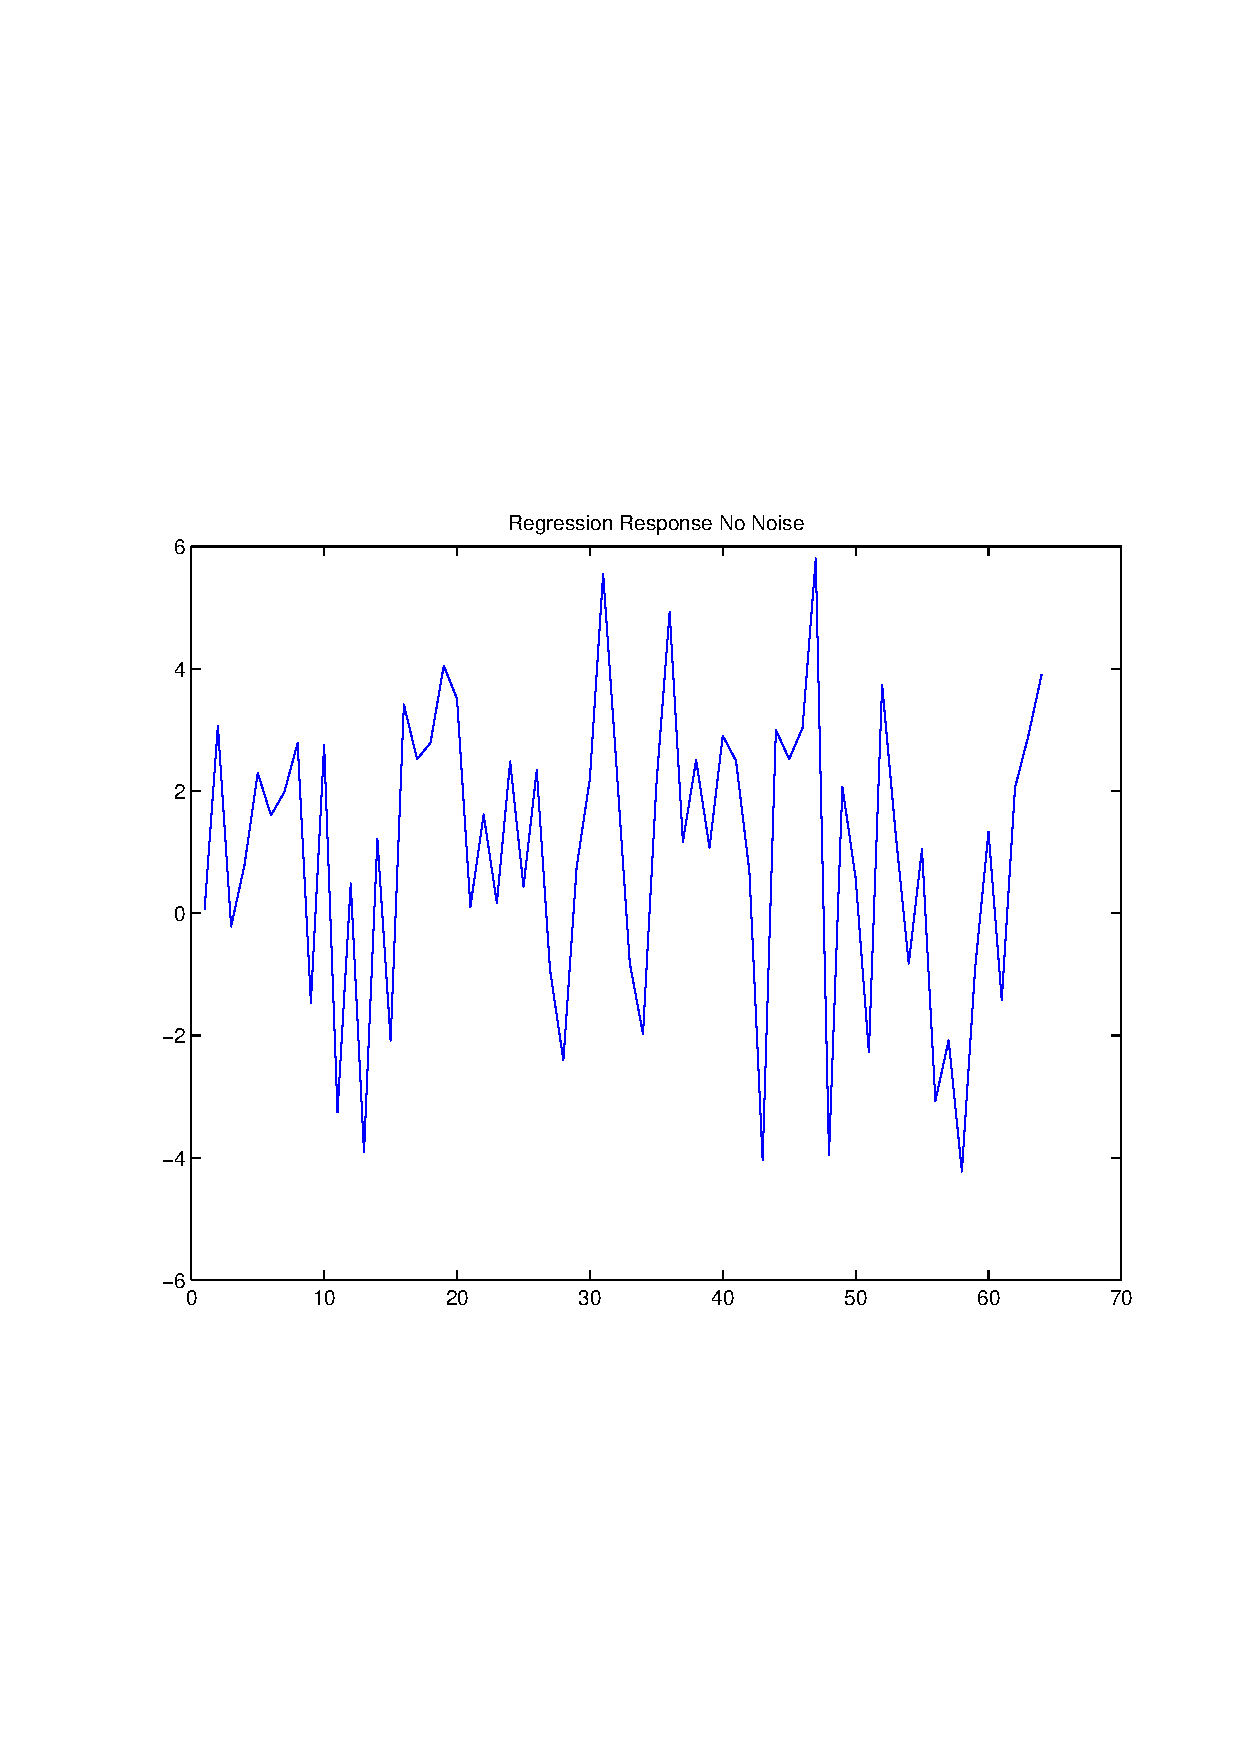
\includegraphics[width=10.0cm,height=10.0cm]{regression_response_no_noise.pdf}

\includegraphics[width=10.0cm,height=10.0cm]{regression_response_with_noise.pdf}

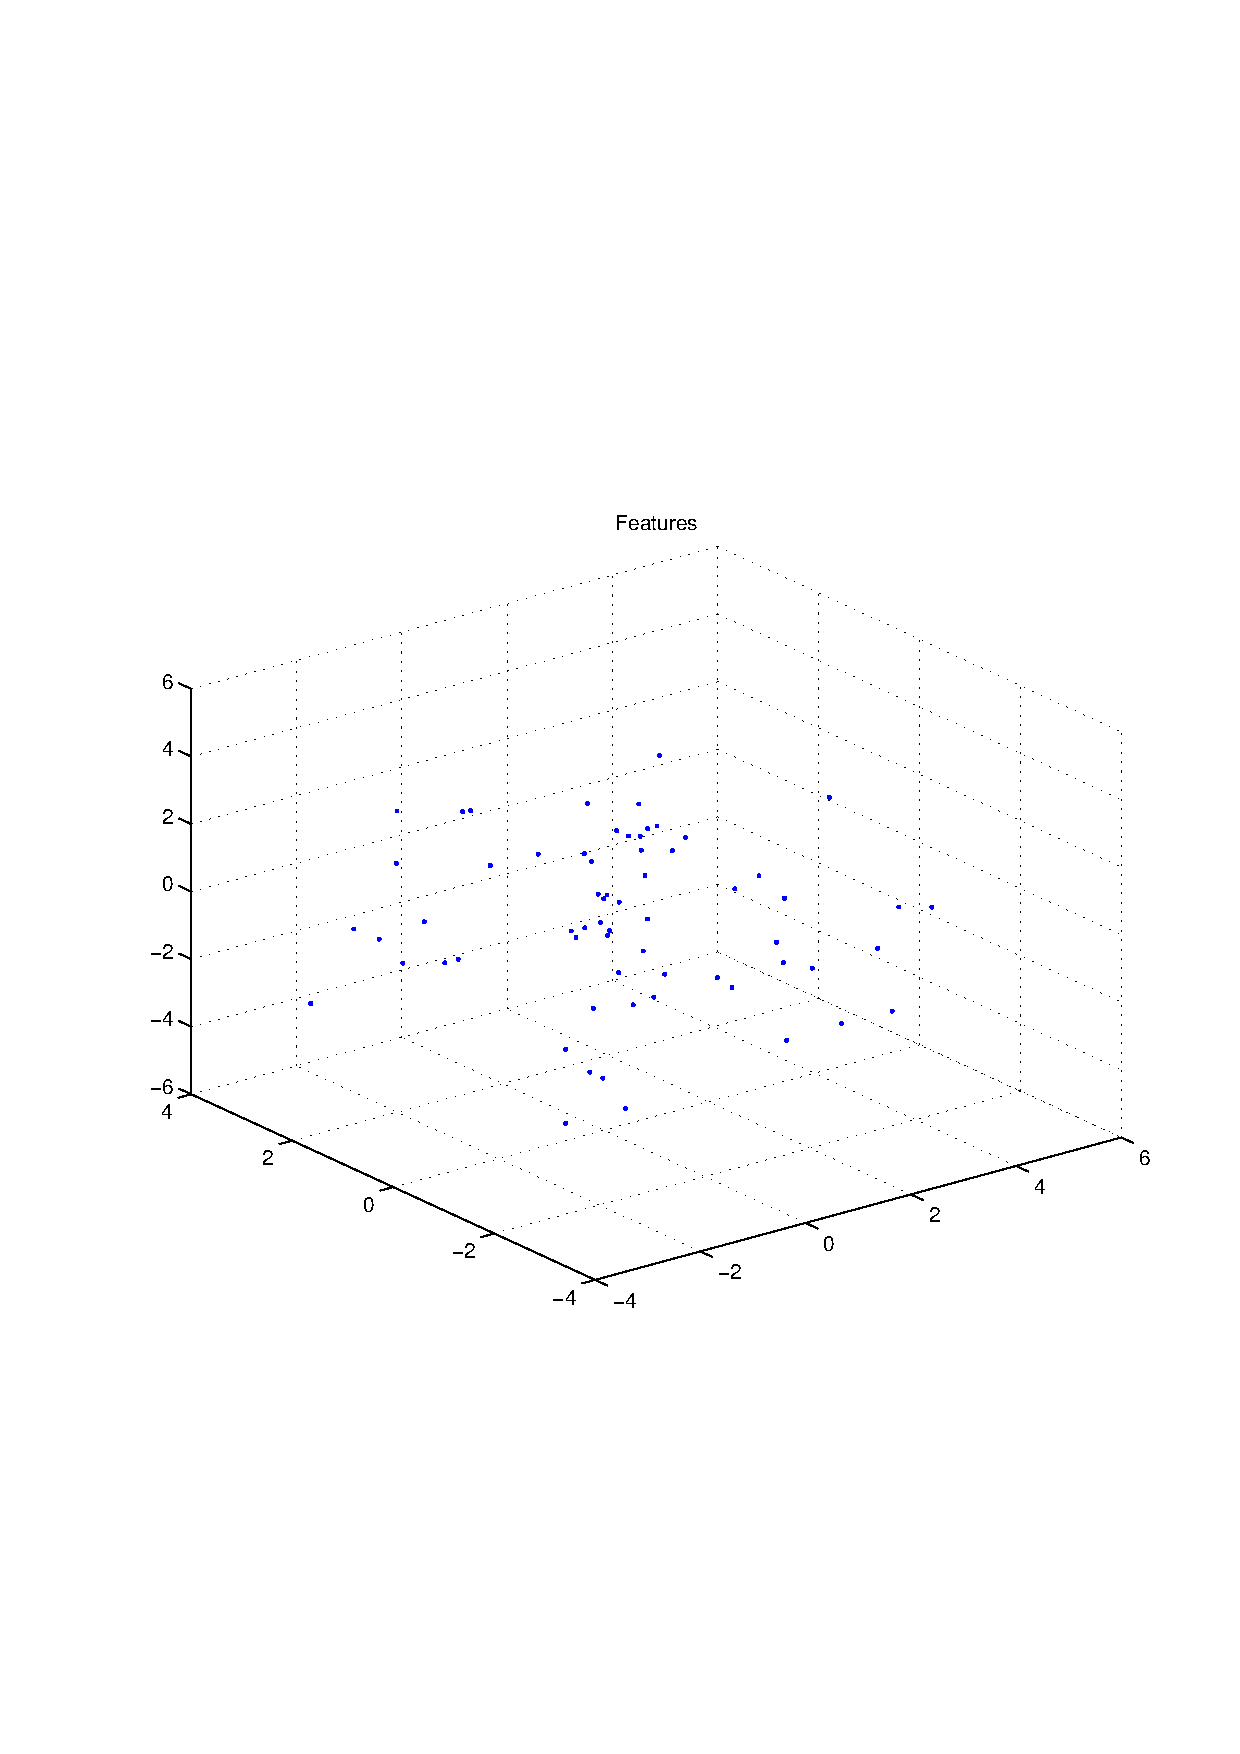
\includegraphics[width=10.0cm,height=10.0cm]{regression_features.pdf}

Beta
+0.817, +0.999, +0.510

Response
+0.062
+3.789
-4.897
+1.656
+3.521
+2.847
+0.438
+5.207
-4.388
+0.951
+4.228
+1.947
-3.584
+3.380
+3.809
+2.116
-0.903
+5.722
-2.996
+3.448
+0.715
+3.720
-1.971
+1.257
+0.684
-3.106
+2.581
+1.667
+2.776
-1.346
+1.858
+2.149
+2.454
+1.135
+4.243
+4.258
-3.697
+0.825
+1.072
+0.542
-0.224
+5.562
-0.759
+1.801
-1.211
+1.547
-0.861
-0.892
+1.019
+3.200
-0.499
-1.228
-0.091
-5.620
+2.604
+0.291
-3.458
+2.237
-1.715
+4.771
-2.169
+3.543
+1.372
+2.429
Estimate for Beta
+0.840
+0.990
+0.512
Error:
+0.022, -0.009, +0.002


QueryPerformanceCounter  =  +2.946
\subsubsection{Fast Gauss Transform}
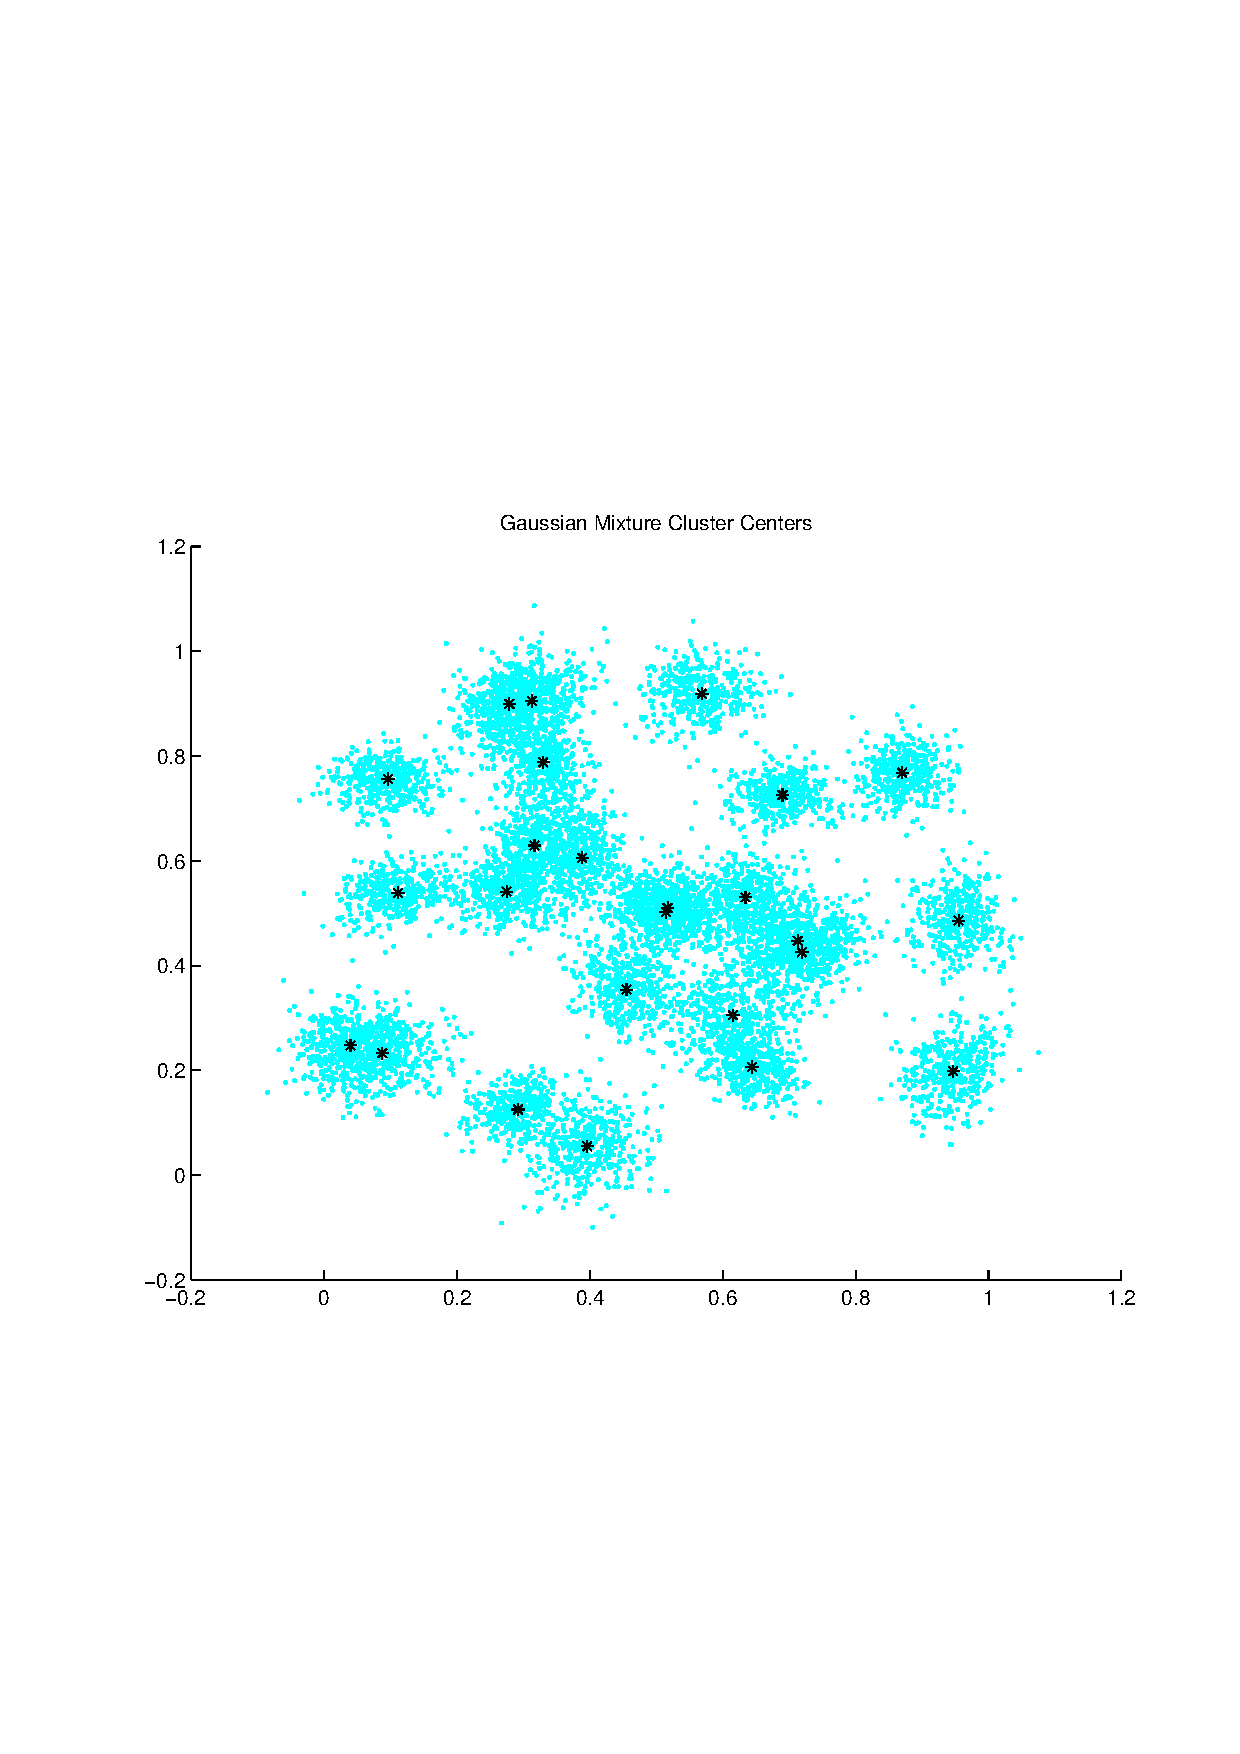
\includegraphics[width=10.0cm,height=10.0cm]{GaussianMixture_ClusterCenters25_Centers.pdf}

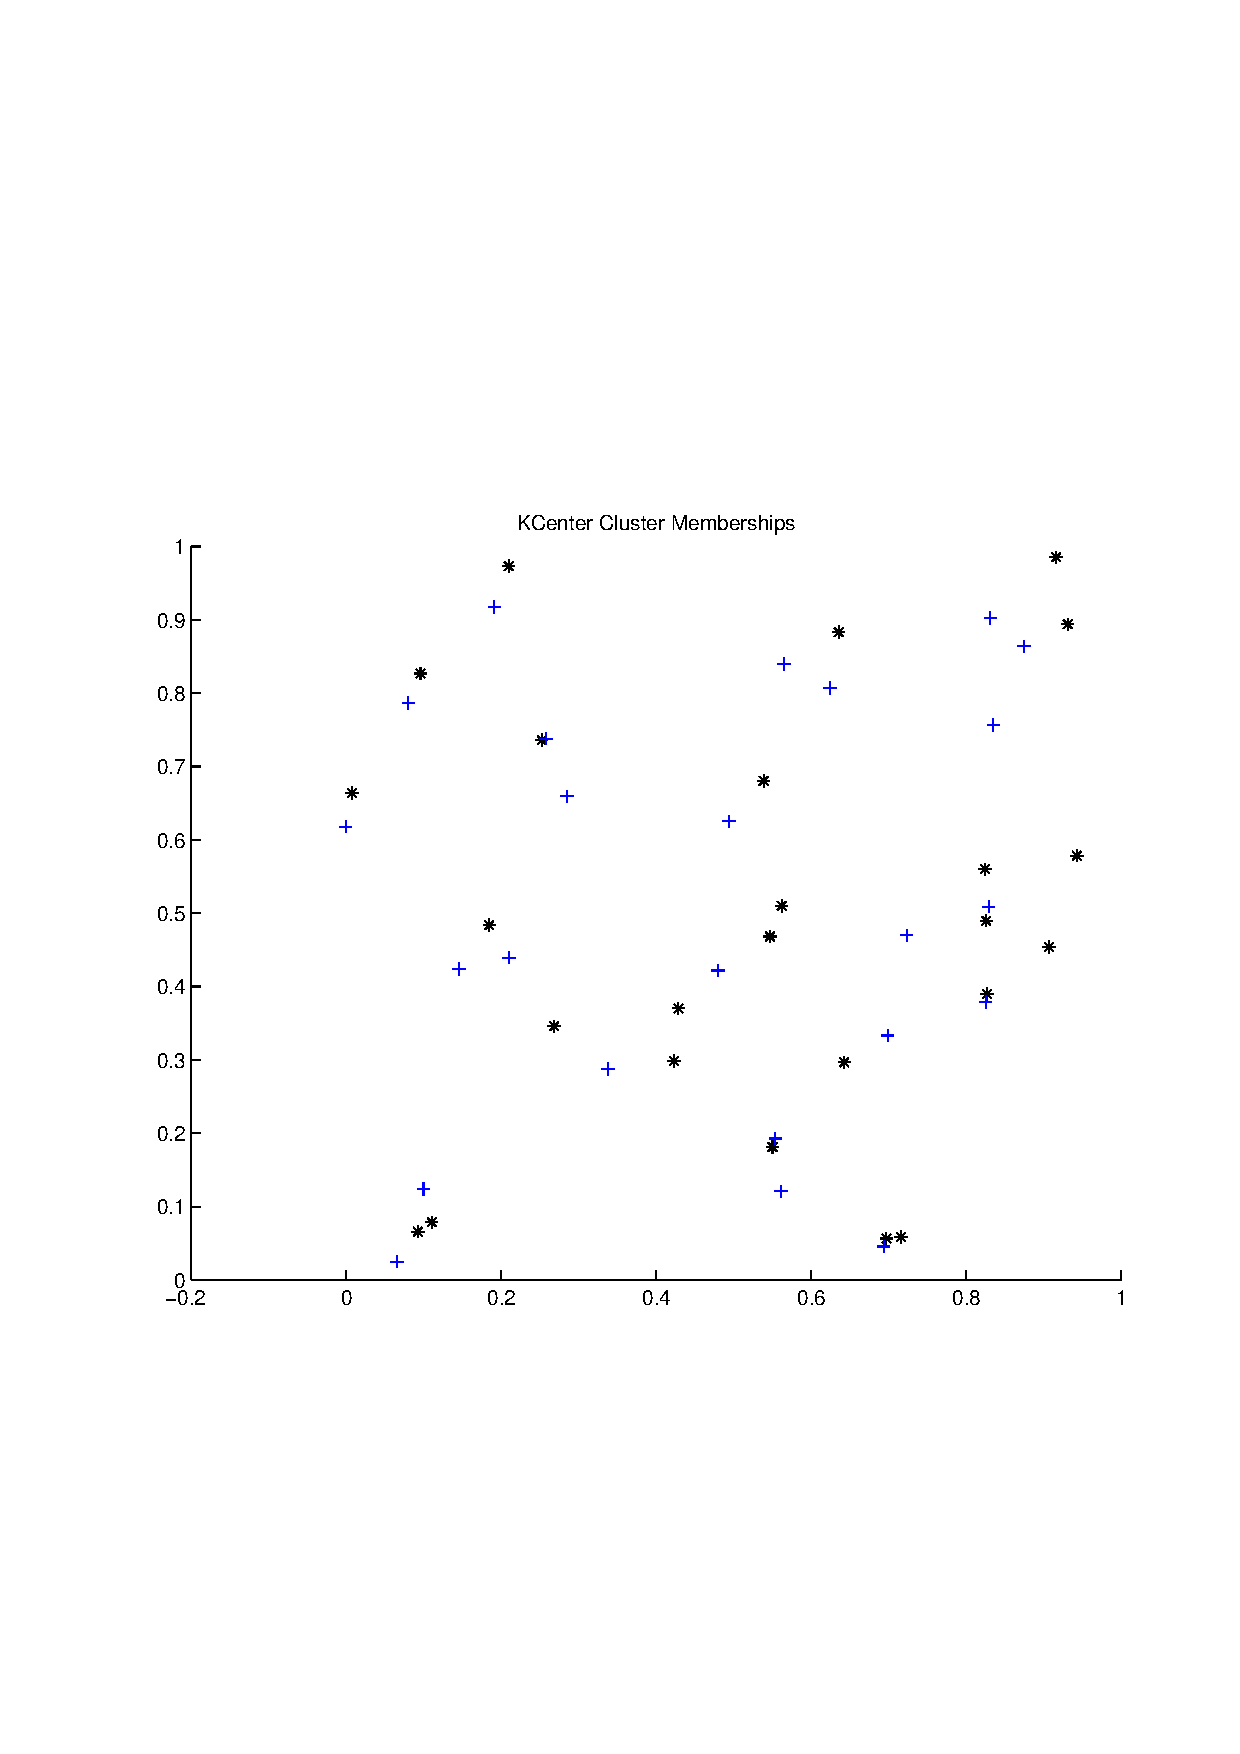
\includegraphics[width=10.0cm,height=10.0cm]{KCenterClusterMemberships_25_Centers.pdf}

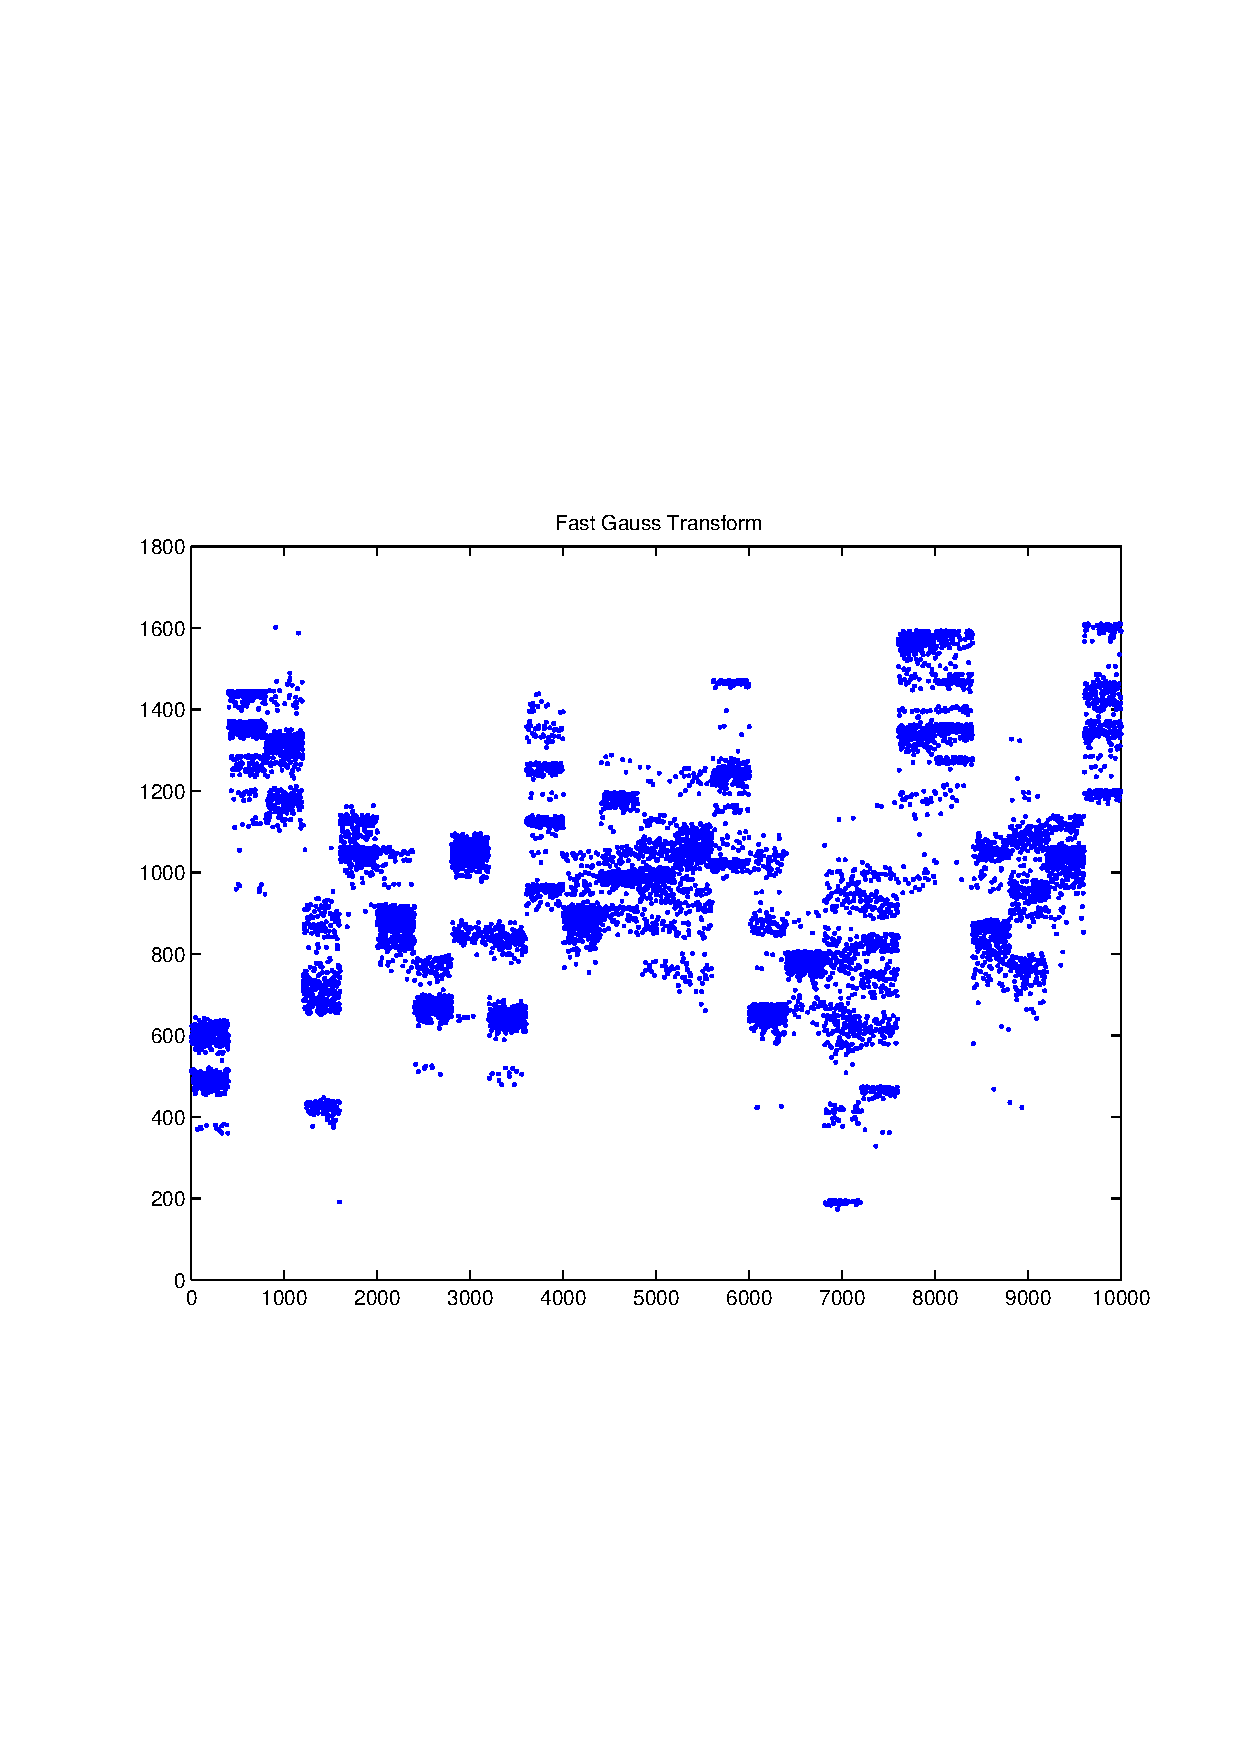
\includegraphics[width=10.0cm,height=10.0cm]{FGT25_Centers.pdf}

QueryPerformanceCounter  =  +7.183
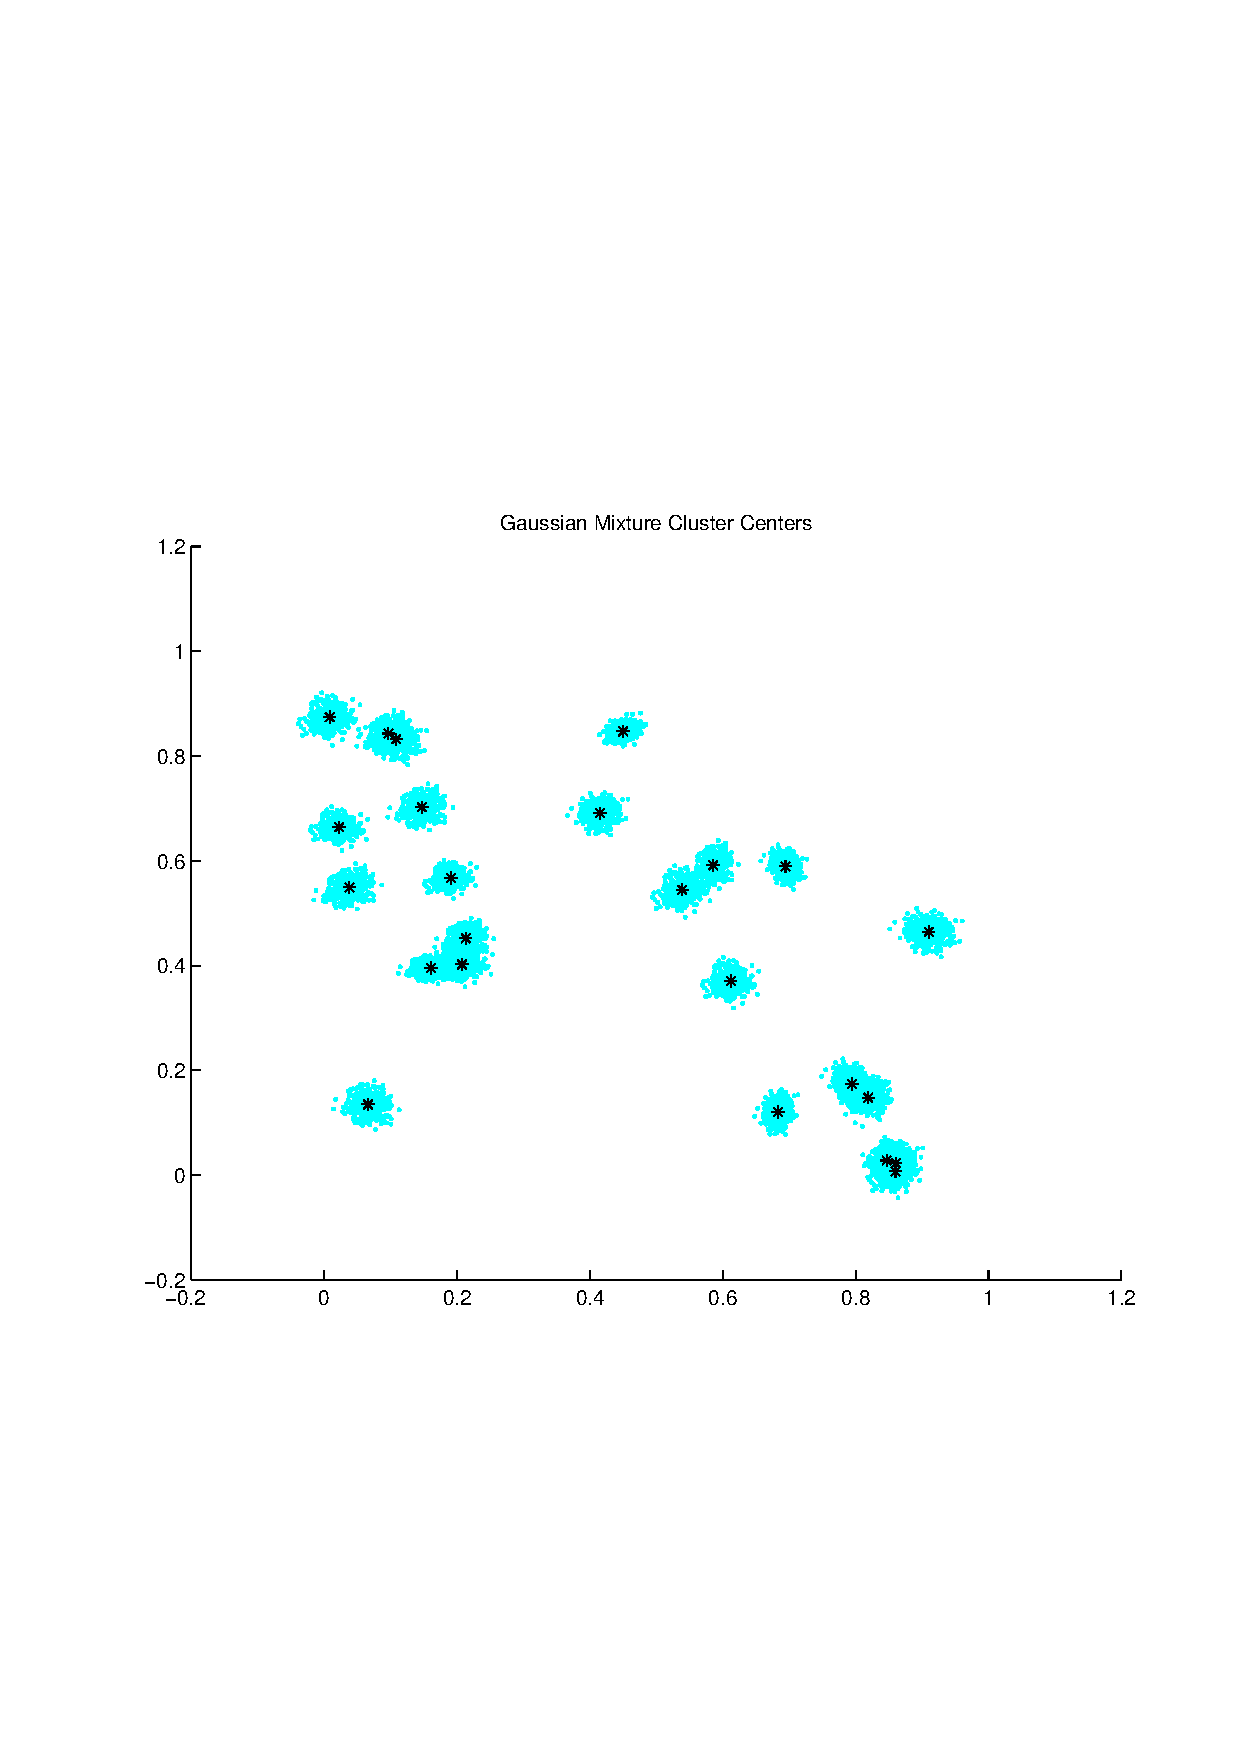
\includegraphics[width=10.0cm,height=10.0cm]{GaussianMixture_ClusterCenters24_Centers.pdf}

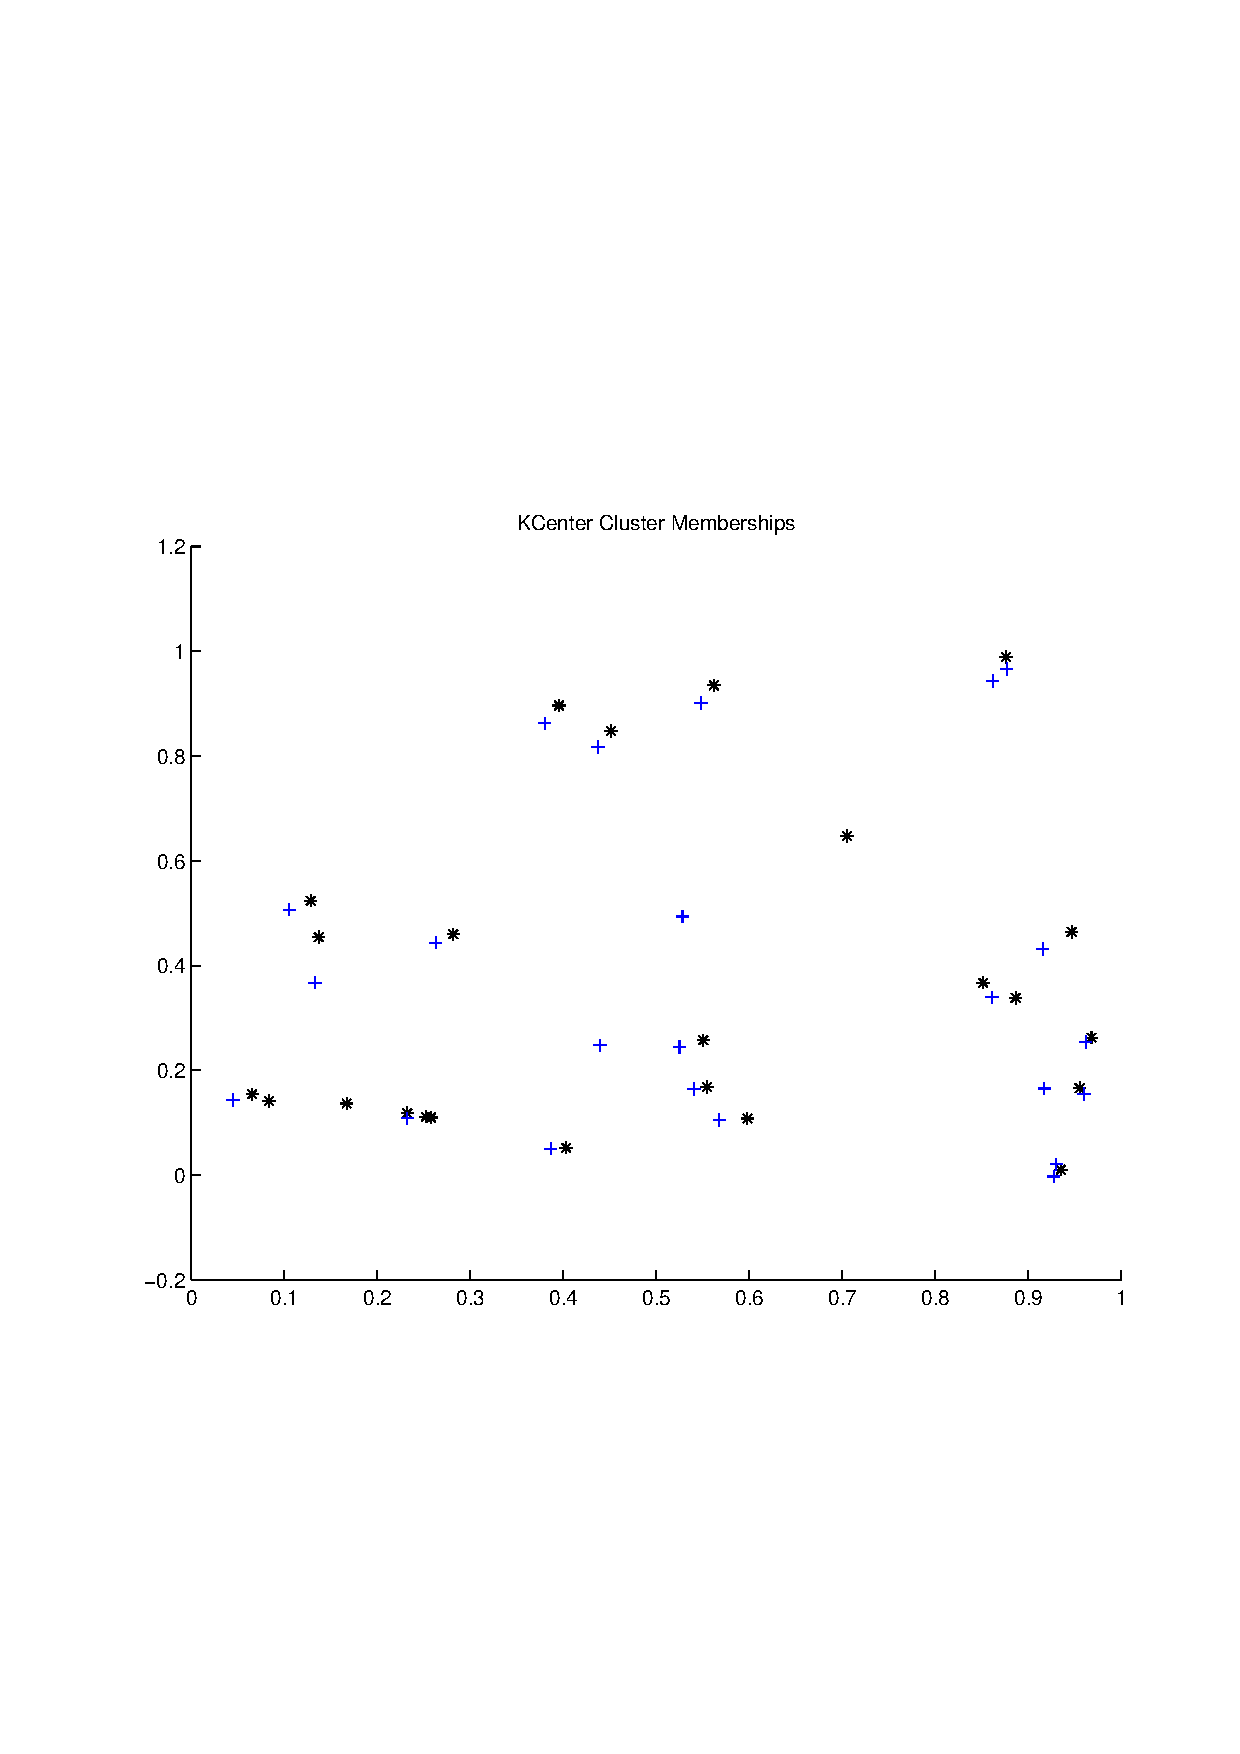
\includegraphics[width=10.0cm,height=10.0cm]{KCenterClusterMemberships_24_Centers.pdf}

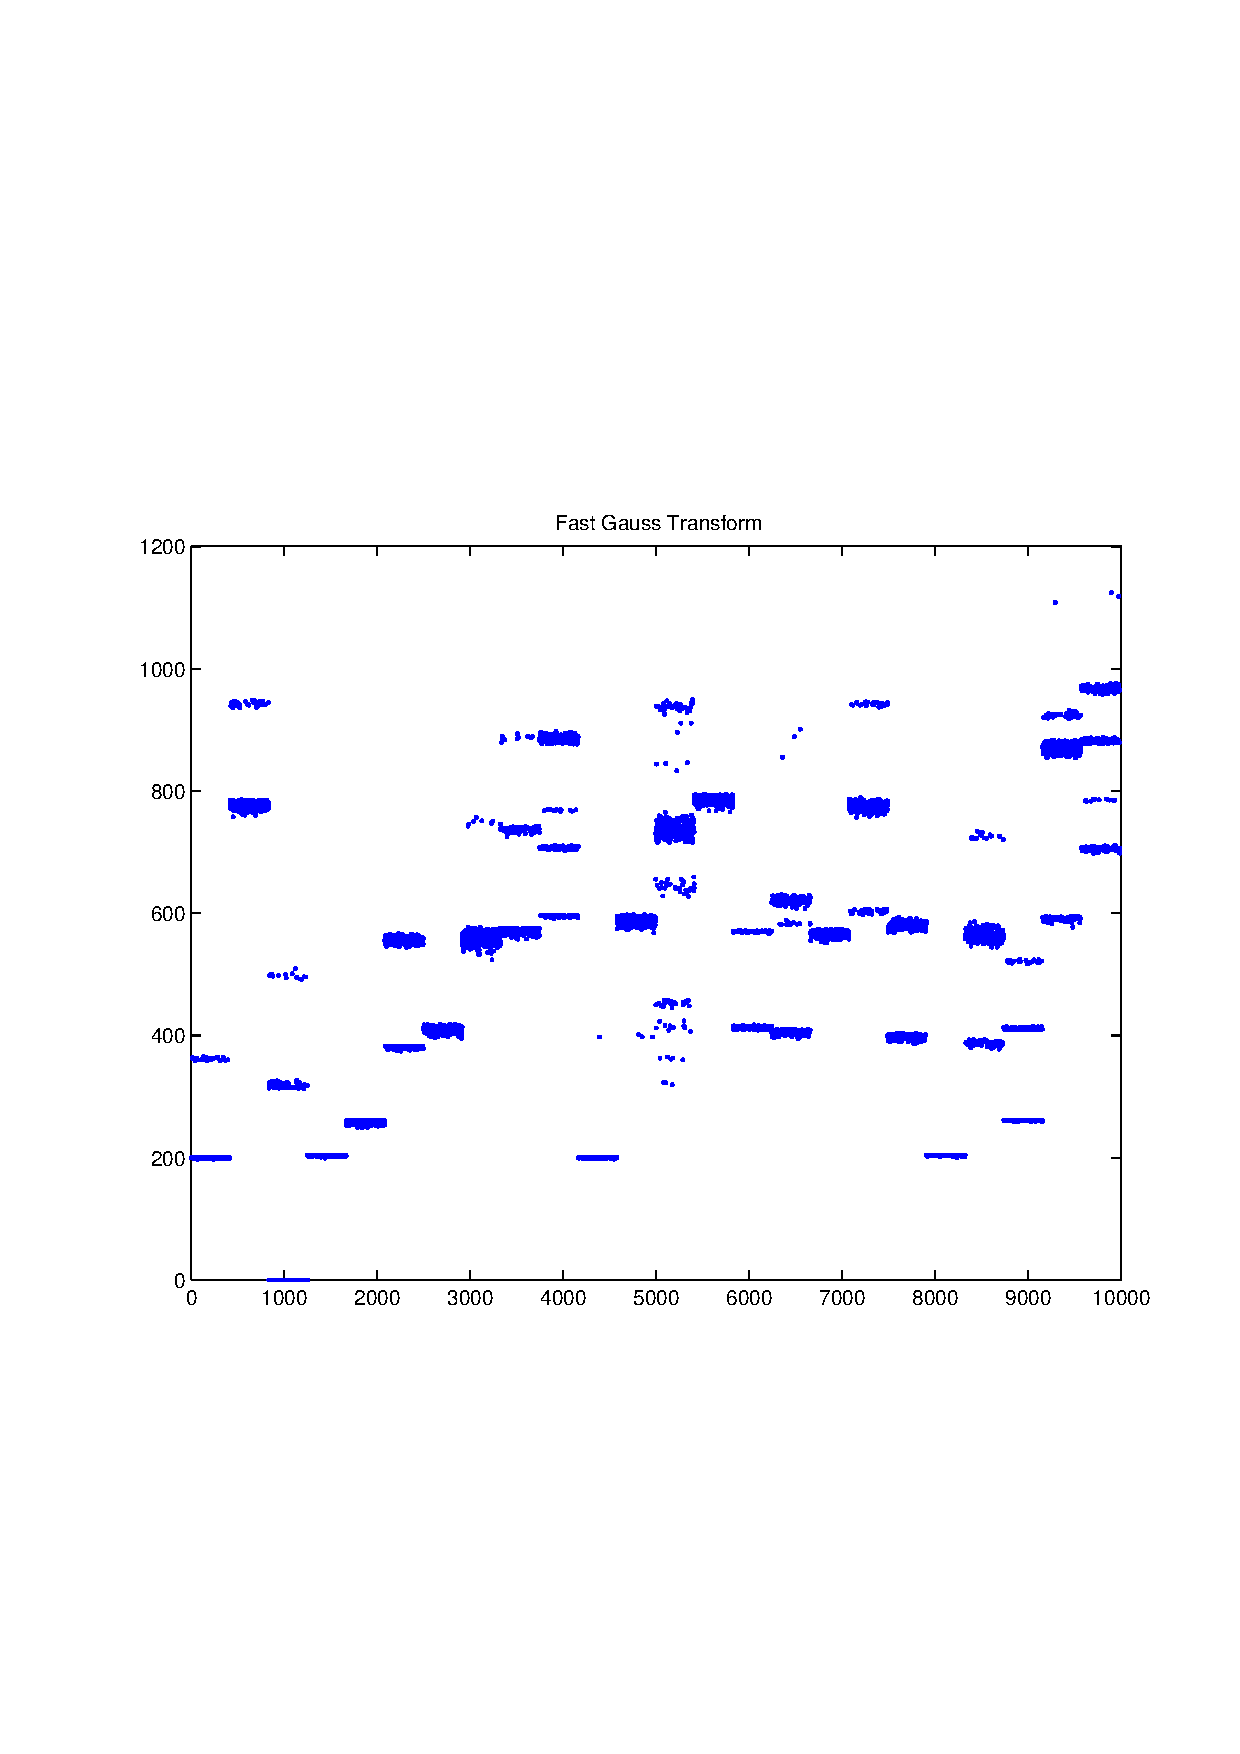
\includegraphics[width=10.0cm,height=10.0cm]{FGT24_Centers.pdf}

QueryPerformanceCounter  =  +7.220
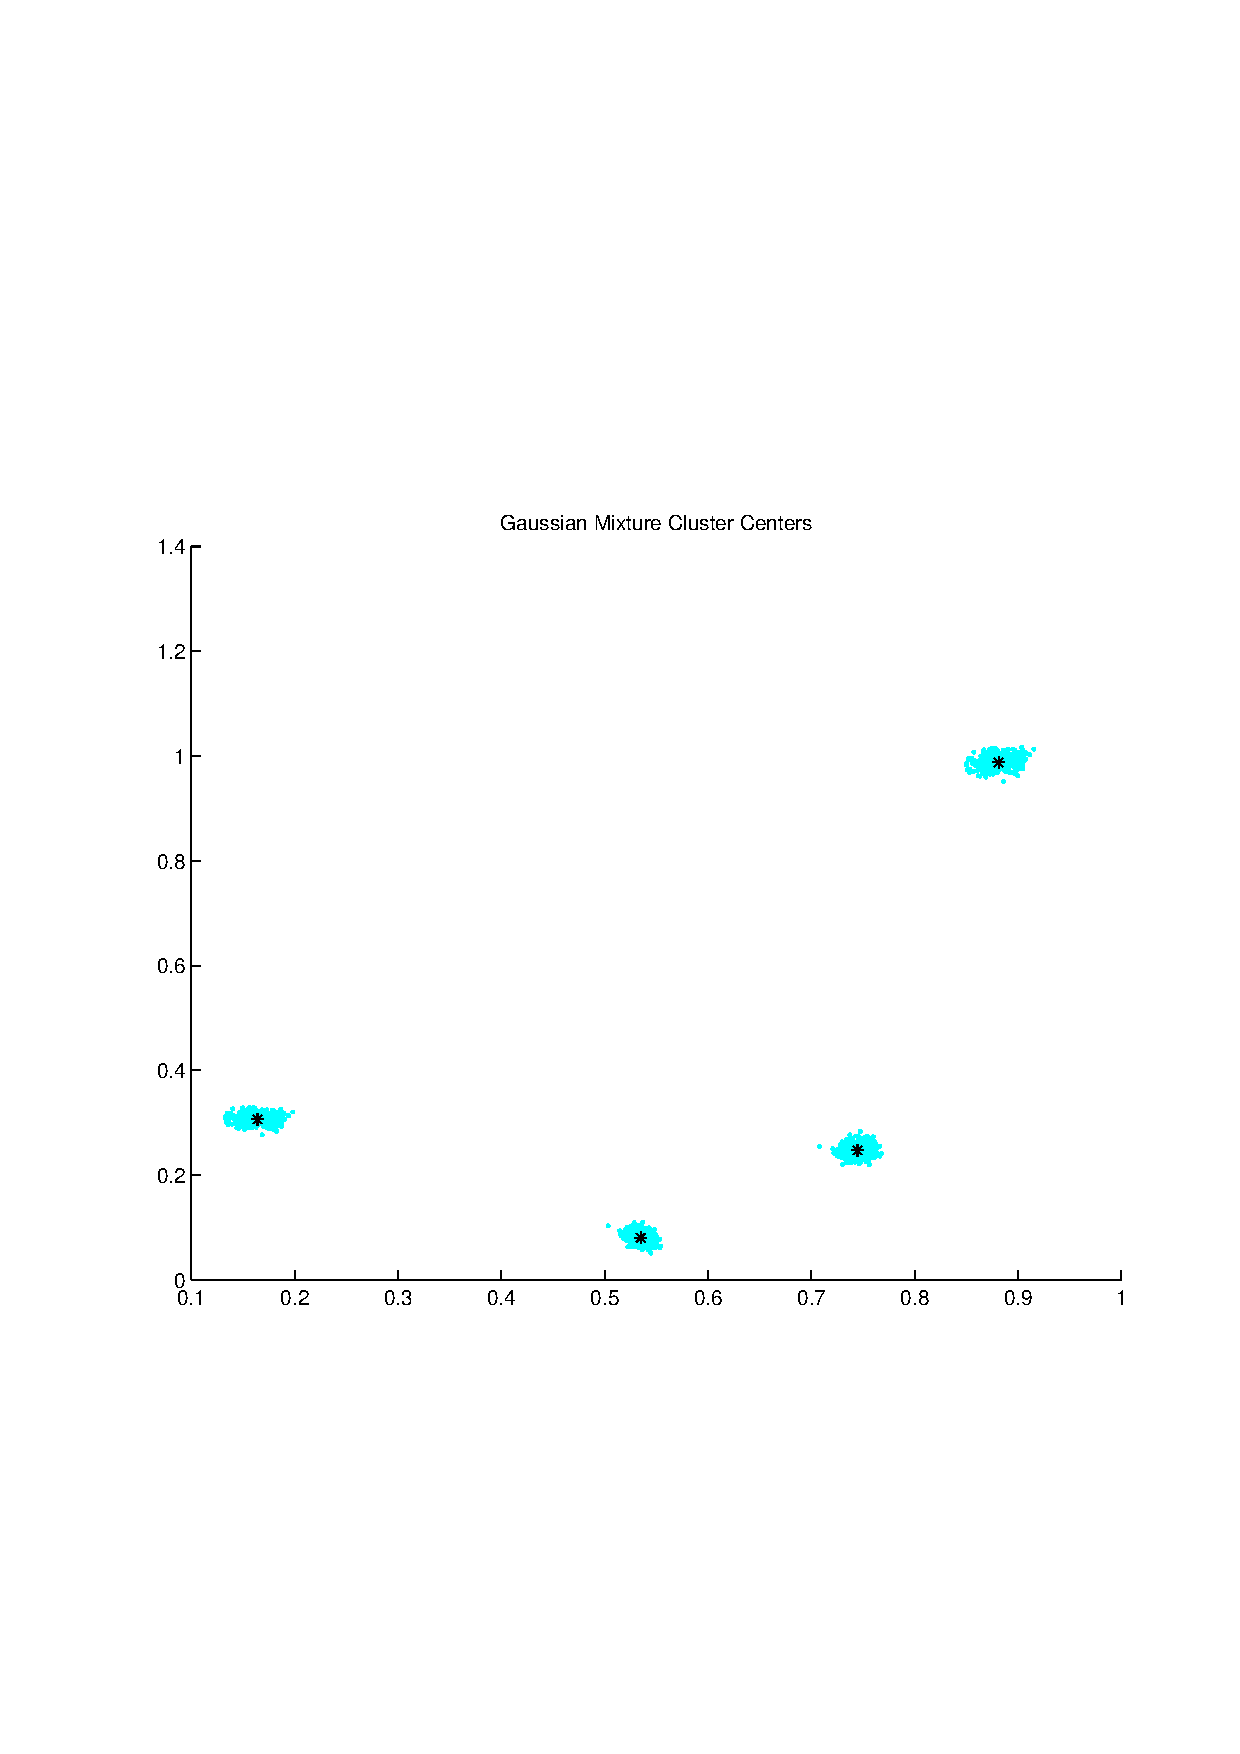
\includegraphics[width=10.0cm,height=10.0cm]{GaussianMixture_ClusterCenters4_Centers.pdf}

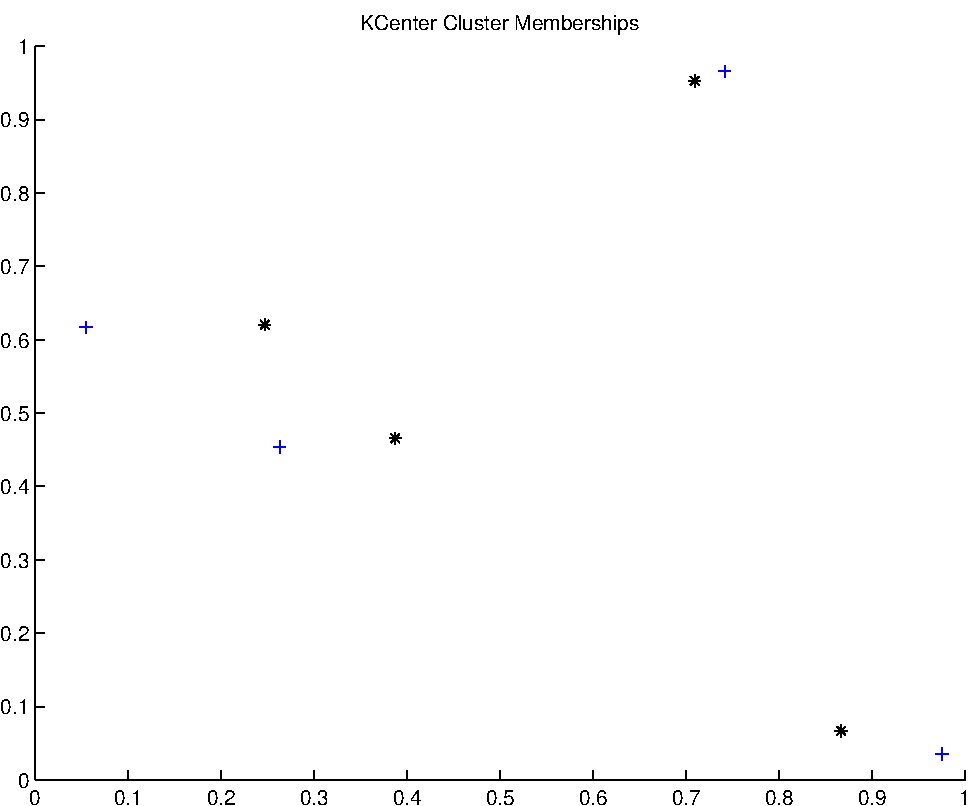
\includegraphics[width=10.0cm,height=10.0cm]{KCenterClusterMemberships_4_Centers.pdf}

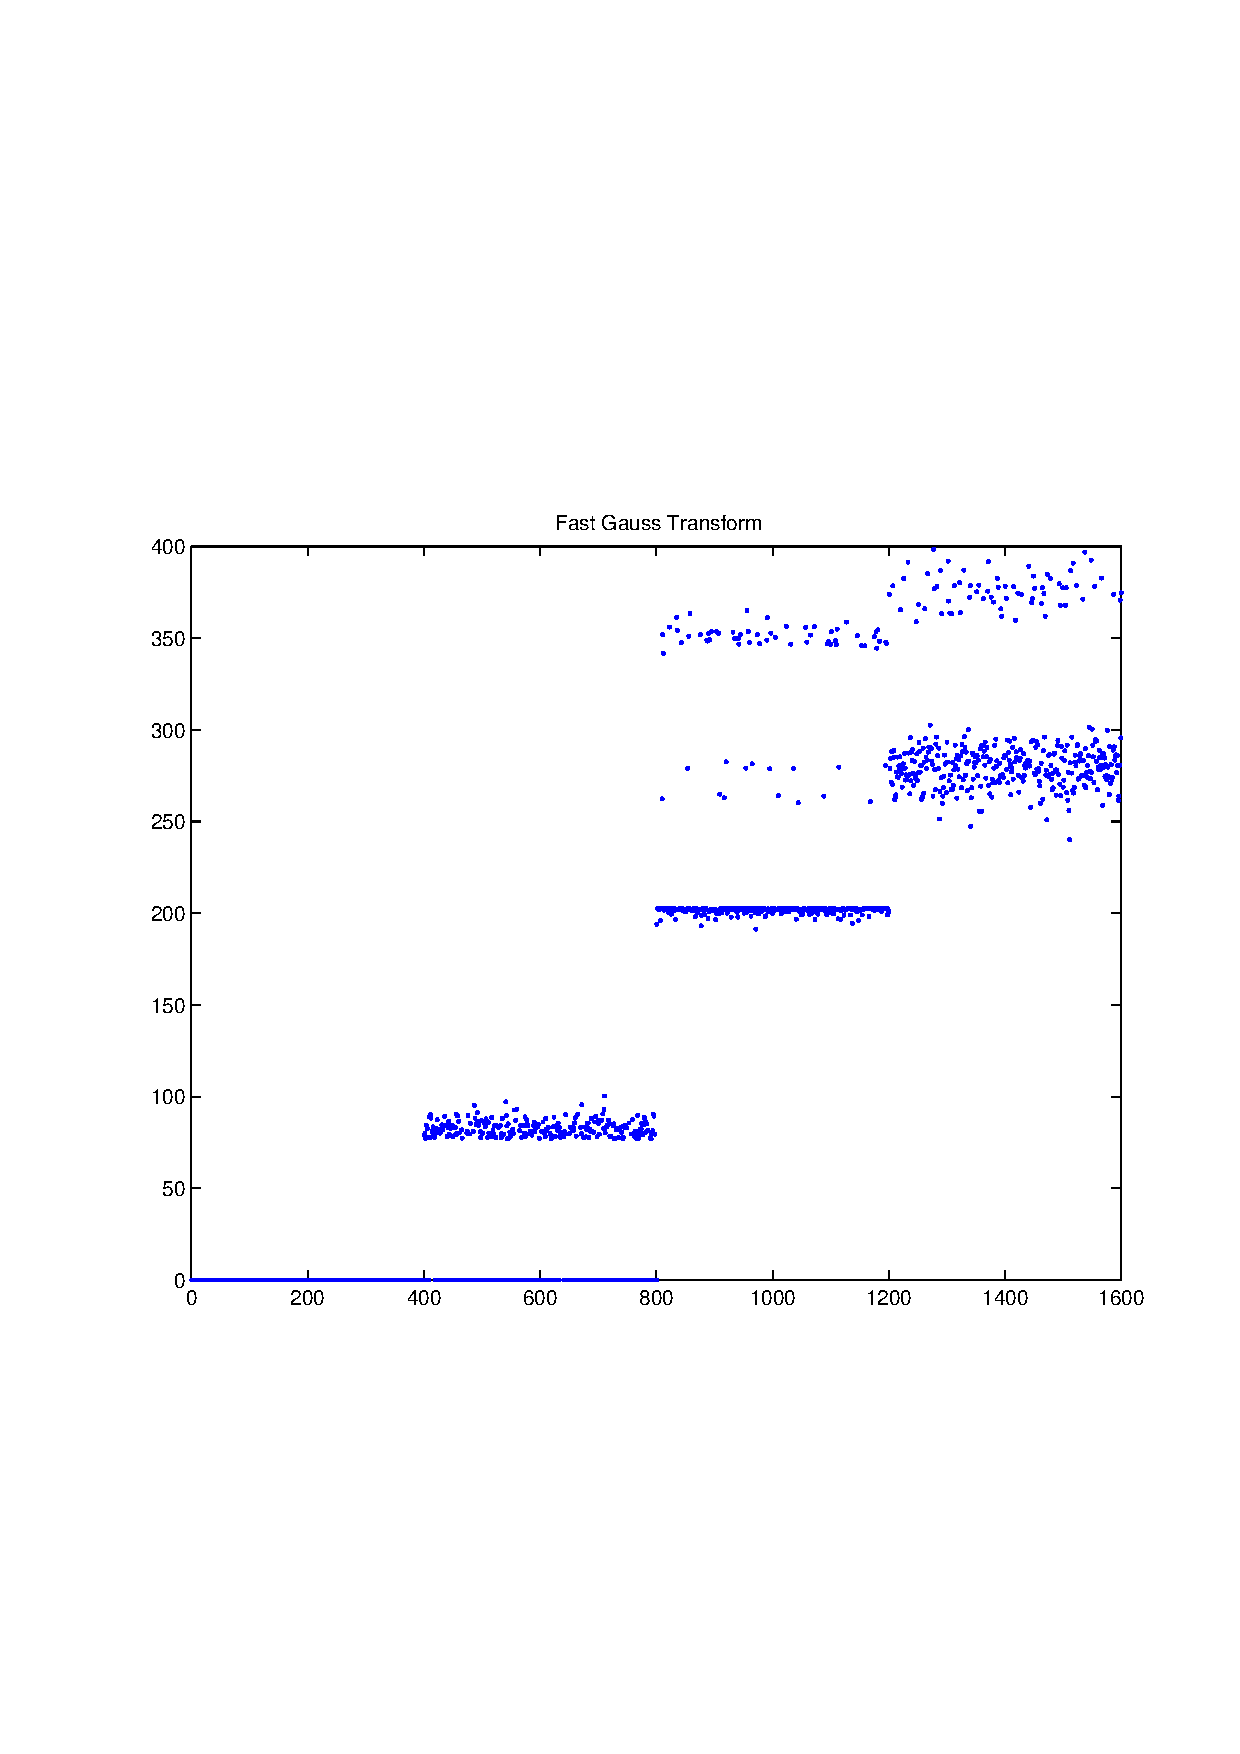
\includegraphics[width=10.0cm,height=10.0cm]{FGT4_Centers.pdf}

QueryPerformanceCounter  =  +3.779
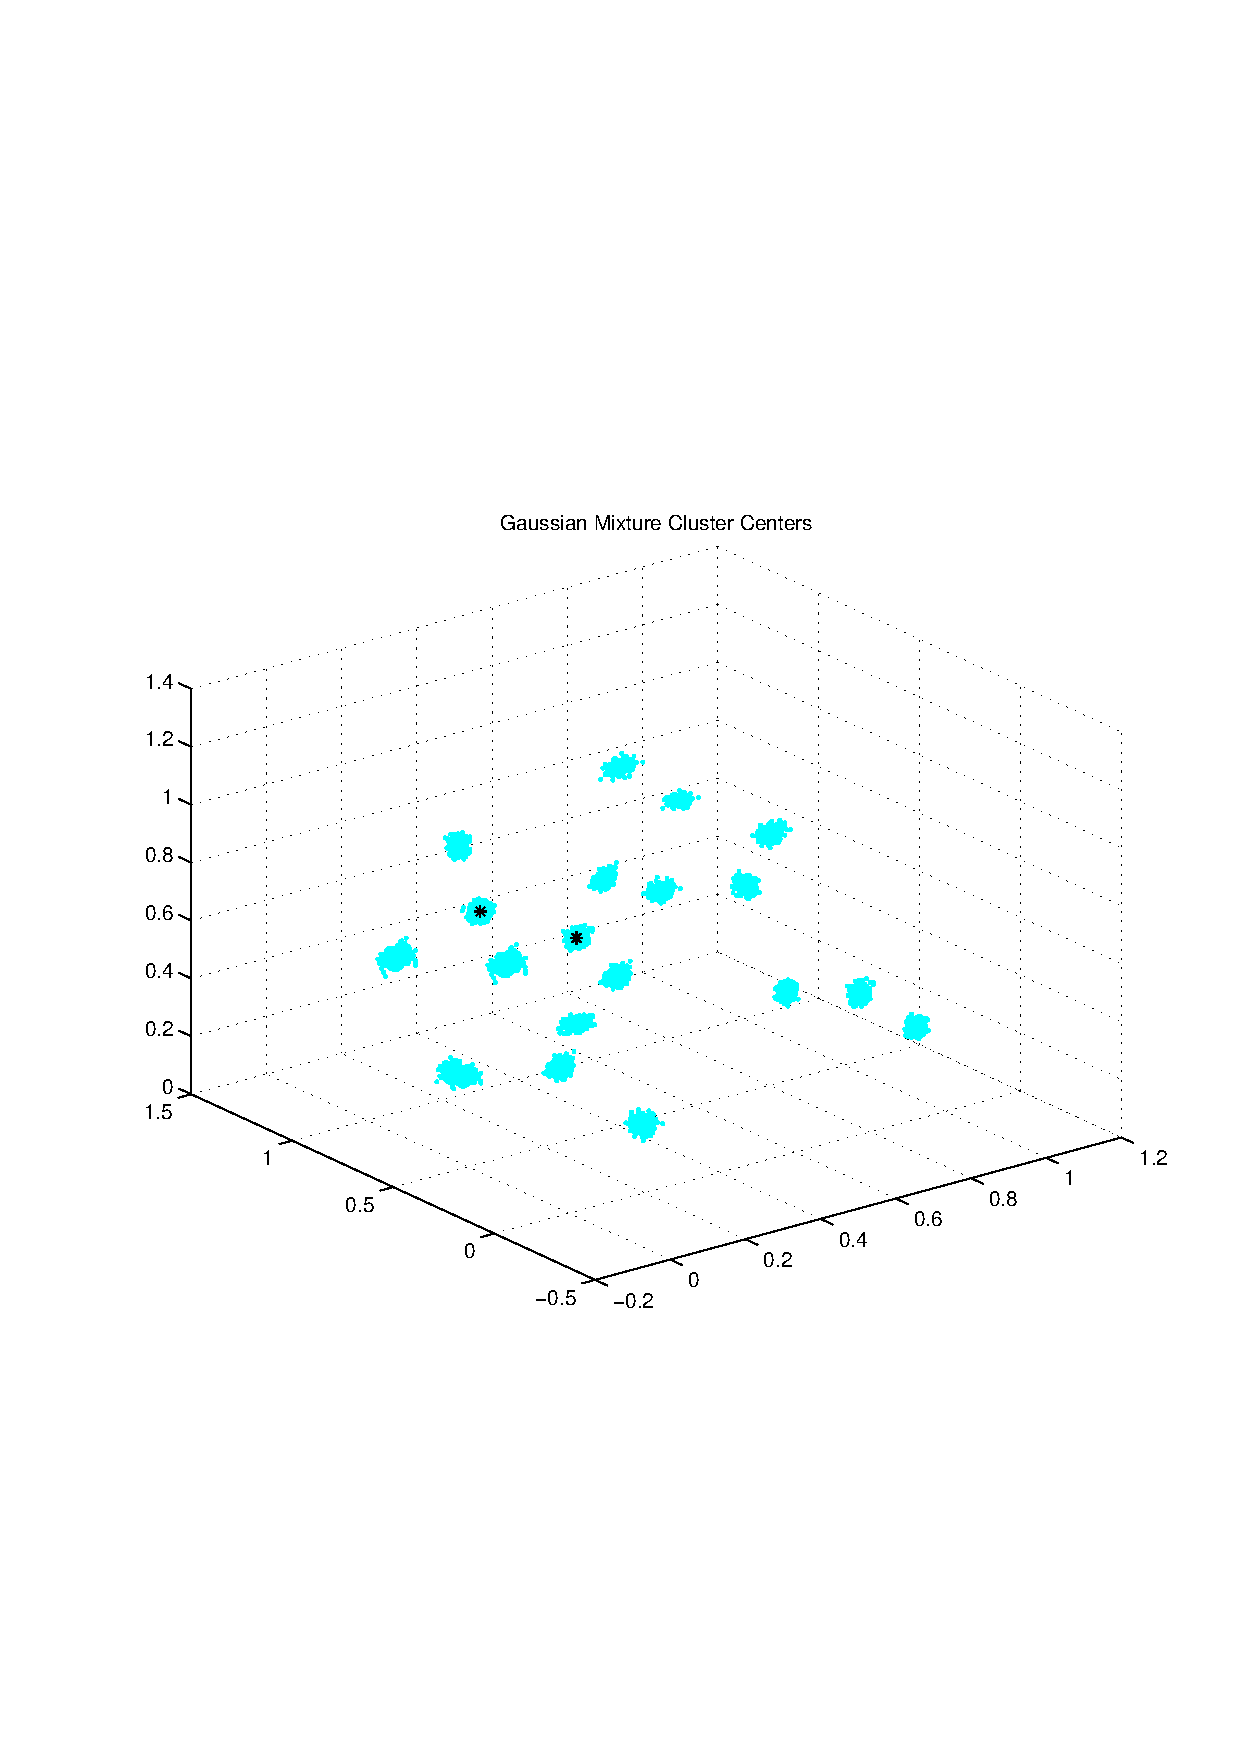
\includegraphics[width=10.0cm,height=10.0cm]{GaussianMixture_ClusterCenters20_Centers.pdf}

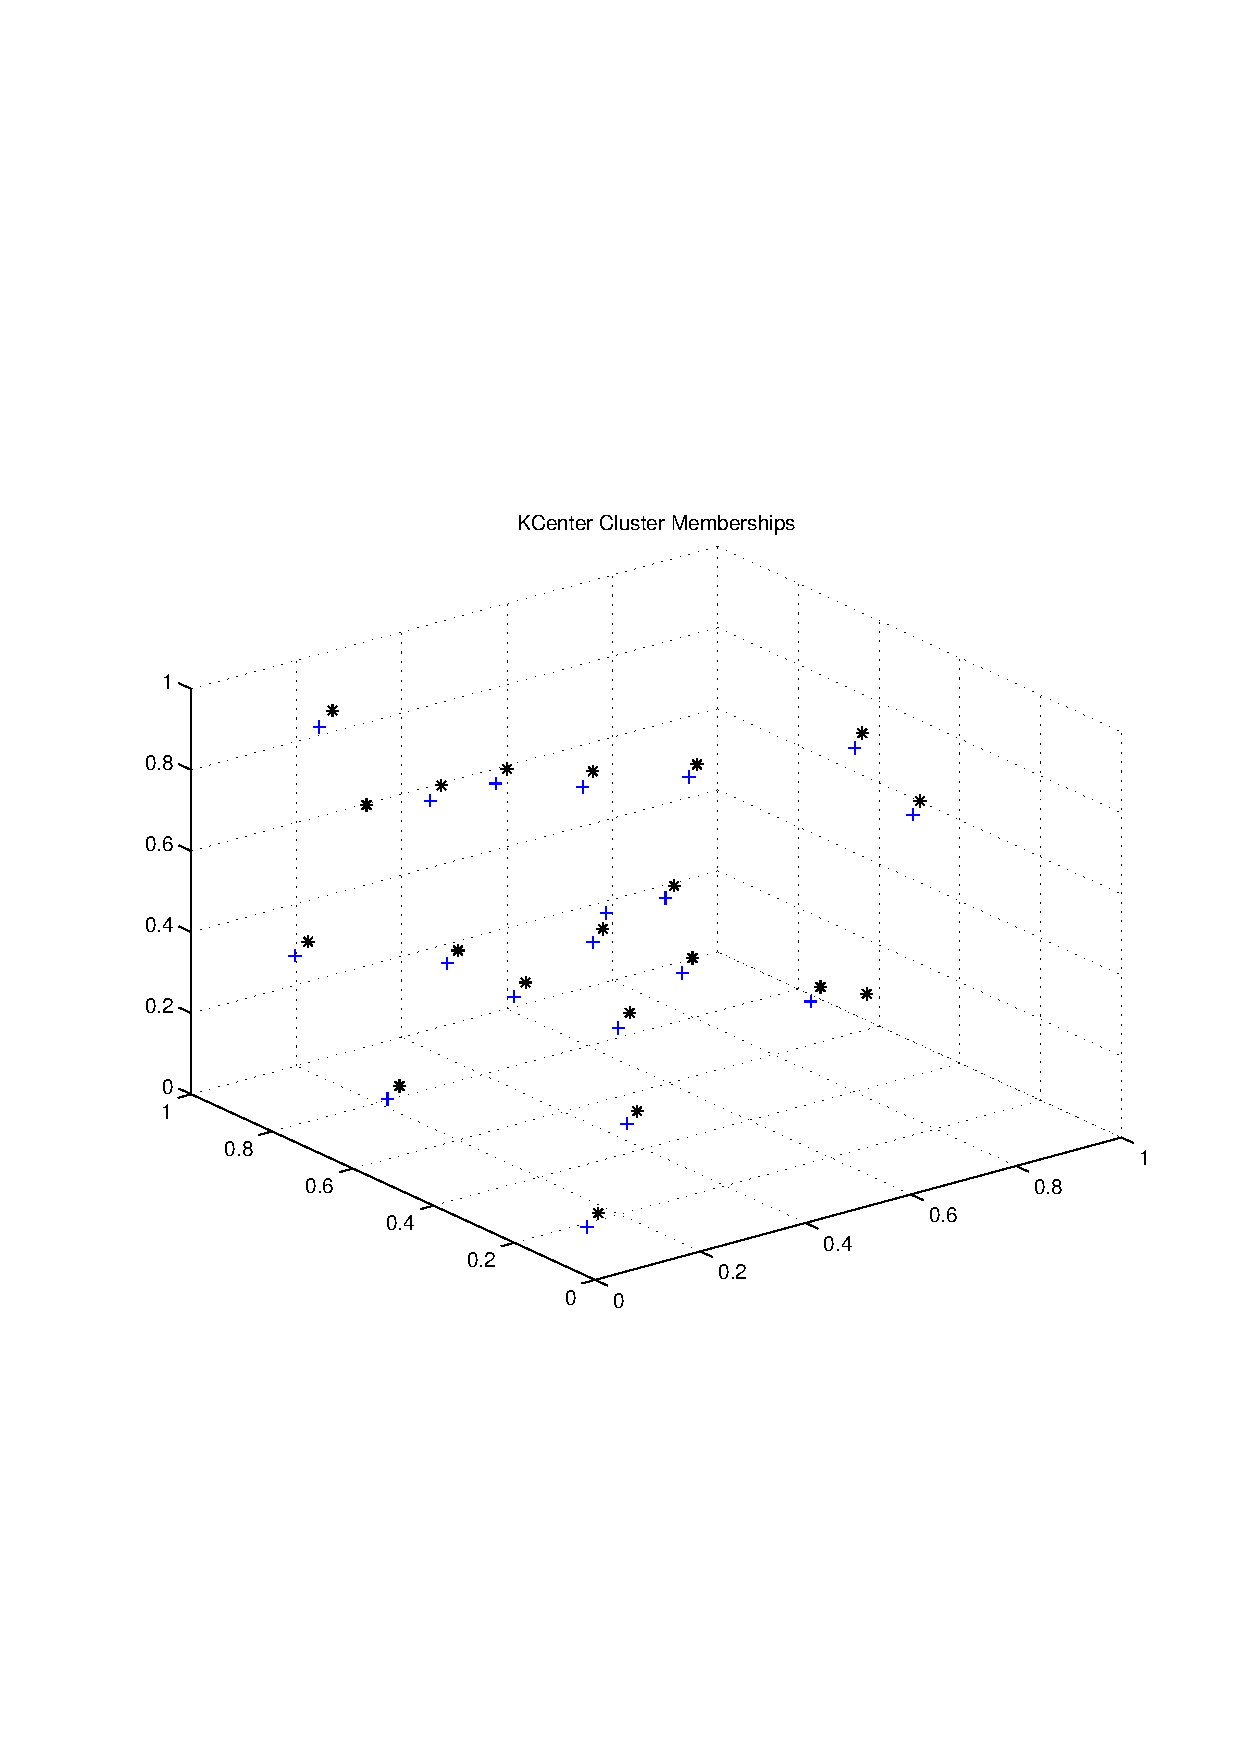
\includegraphics[width=10.0cm,height=10.0cm]{KCenterClusterMemberships_20_Centers.pdf}

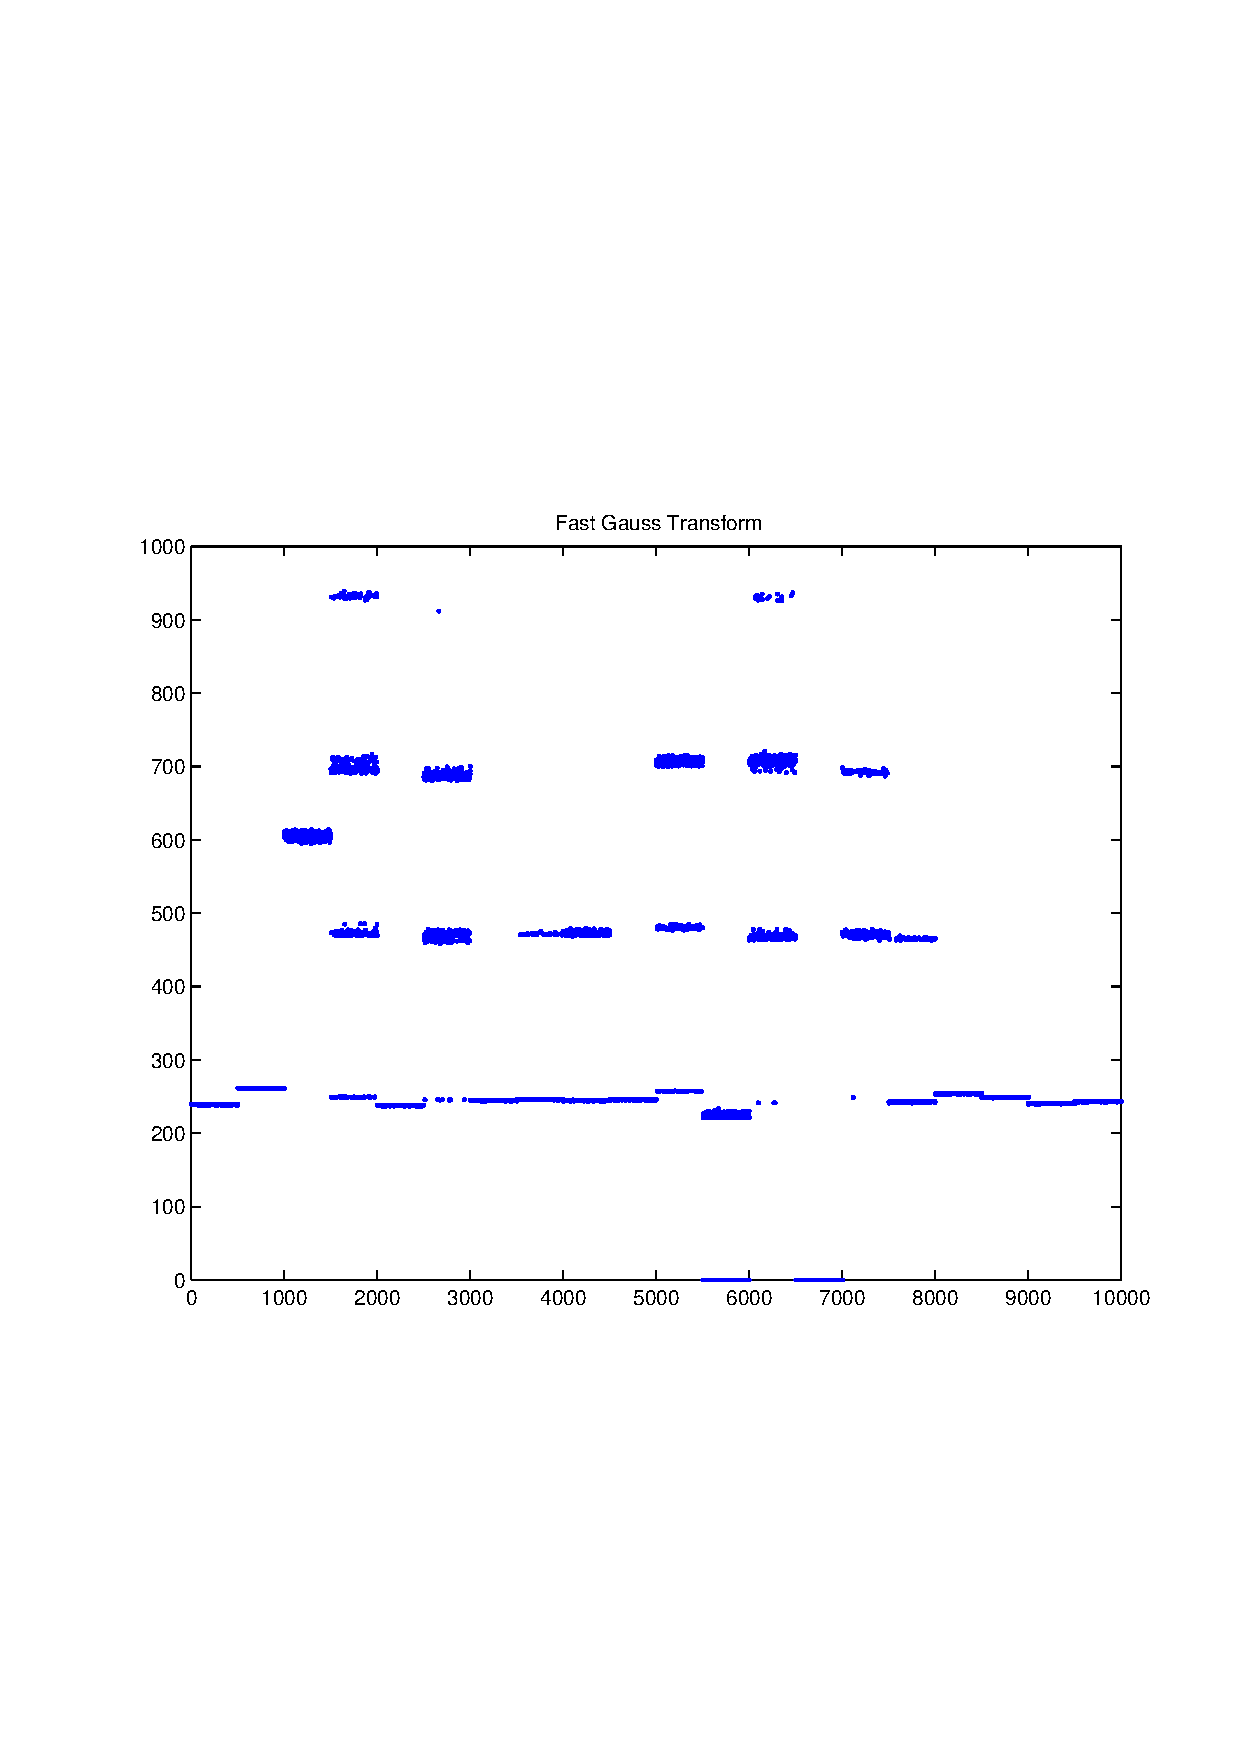
\includegraphics[width=10.0cm,height=10.0cm]{FGT20_Centers.pdf}

QueryPerformanceCounter  =  +6.471
\subsubsection{Matrix Norms}
\subsubsection{Haar Distributed Random Orthogonal Matrix $A \in O(n)$}
 Testing Operator Norm
Number of Dimensions: +12

$A = \left(
\begin{array}{
cccccccccccc}
-0.006 & +0.322 & +0.226 & +0.111 & +0.046 & -0.448 & -0.499 & -0.352 & -0.254 & +0.060 & +0.428 & -0.071 \\
+0.105 & -0.339 & -0.059 & +0.525 & -0.140 & +0.224 & -0.143 & +0.271 & -0.185 & -0.130 & +0.273 & -0.553 \\
-0.008 & -0.072 & +0.555 & -0.005 & +0.227 & -0.233 & +0.171 & +0.201 & +0.237 & +0.532 & -0.139 & -0.390 \\
-0.357 & +0.337 & +0.183 & +0.225 & +0.490 & +0.450 & +0.055 & -0.274 & +0.181 & -0.296 & -0.037 & -0.179 \\
+0.261 & +0.371 & -0.203 & -0.009 & +0.413 & -0.286 & +0.374 & +0.352 & -0.419 & -0.207 & -0.025 & -0.134 \\
+0.085 & -0.101 & -0.168 & +0.063 & +0.084 & -0.405 & -0.393 & -0.033 & +0.322 & -0.379 & -0.564 & -0.241 \\
-0.159 & -0.507 & +0.327 & -0.181 & +0.002 & -0.260 & +0.383 & -0.314 & -0.208 & -0.457 & +0.100 & -0.057 \\
-0.061 & -0.339 & -0.495 & +0.304 & +0.449 & -0.223 & +0.156 & -0.263 & +0.202 & +0.302 & +0.221 & +0.136 \\
+0.663 & +0.173 & +0.038 & -0.042 & -0.144 & +0.038 & +0.248 & -0.254 & +0.495 & -0.160 & +0.297 & -0.141 \\
-0.549 & +0.235 & -0.174 & -0.019 & -0.307 & -0.309 & +0.190 & +0.309 & +0.383 & -0.153 & +0.325 & -0.124 \\
+0.125 & -0.128 & +0.369 & +0.289 & +0.221 & -0.071 & -0.147 & +0.435 & +0.214 & -0.264 & +0.176 & +0.581 \\
-0.008 & +0.203 & +0.116 & +0.669 & -0.380 & -0.165 & +0.337 & -0.213 & -0.107 & +0.067 & -0.343 & +0.184 \\
\end{array}
\right)$ \newline 

$Det(A) :   A \in O(n)$ = (-1.000,+0.000)

$L = \left(
\begin{array}{
cccccccccccc}
+1.000 & +0.000 & +0.000 & +0.000 & +0.000 & +0.000 & +0.000 & +0.000 & +0.000 & +0.000 & +0.000 & +0.000 \\
-0.239 & +1.000 & +0.000 & +0.000 & +0.000 & +0.000 & +0.000 & +0.000 & +0.000 & +0.000 & +0.000 & +0.000 \\
-0.092 & +0.694 & +1.000 & +0.000 & +0.000 & +0.000 & +0.000 & +0.000 & +0.000 & +0.000 & +0.000 & +0.000 \\
-0.013 & -0.440 & -0.365 & +1.000 & +0.000 & +0.000 & +0.000 & +0.000 & +0.000 & +0.000 & +0.000 & +0.000 \\
-0.538 & -0.923 & -0.709 & +0.449 & +1.000 & +0.000 & +0.000 & +0.000 & +0.000 & +0.000 & +0.000 & +0.000 \\
-0.009 & -0.695 & -0.635 & +0.341 & +0.482 & +1.000 & +0.000 & +0.000 & +0.000 & +0.000 & +0.000 & +0.000 \\
+0.158 & +0.788 & +0.455 & +0.654 & -0.185 & -0.964 & +1.000 & +0.000 & +0.000 & +0.000 & +0.000 & +0.000 \\
+0.393 & -0.651 & -0.001 & -0.156 & +0.509 & +0.955 & -0.807 & +1.000 & +0.000 & +0.000 & +0.000 & +0.000 \\
-0.011 & +0.151 & -0.696 & +0.438 & +0.801 & +0.516 & +0.098 & +0.852 & +1.000 & +0.000 & +0.000 & +0.000 \\
-0.828 & -0.812 & -0.181 & -0.175 & -0.506 & +0.517 & -0.973 & +0.065 & +0.657 & +1.000 & +0.000 & +0.000 \\
+0.127 & +0.264 & +0.360 & -0.050 & -0.081 & +0.441 & +0.150 & +0.043 & +0.443 & +0.740 & +1.000 & +0.000 \\
+0.188 & +0.345 & -0.339 & +0.686 & +0.705 & +0.064 & +0.687 & +0.835 & +0.997 & +0.521 & +0.416 & +1.000 \\
\end{array}
\right)$ \newline 

$U = \left(
\begin{array}{
cccccccccccc}
+0.663 & +0.173 & +0.038 & -0.042 & -0.144 & +0.038 & +0.248 & -0.254 & +0.495 & -0.160 & +0.297 & -0.141 \\
+0.000 & -0.466 & +0.336 & -0.191 & -0.032 & -0.251 & +0.442 & -0.375 & -0.090 & -0.495 & +0.172 & -0.091 \\
+0.000 & +0.000 & -0.725 & +0.432 & +0.458 & -0.045 & -0.128 & -0.026 & +0.310 & +0.630 & +0.130 & +0.187 \\
+0.000 & +0.000 & +0.000 & +0.742 & -0.230 & -0.291 & +0.488 & -0.391 & -0.027 & +0.077 & -0.217 & +0.210 \\
+0.000 & +0.000 & +0.000 & +0.000 & +0.811 & +0.338 & +0.286 & -0.599 & +0.596 & -0.427 & +0.470 & -0.302 \\
+0.000 & +0.000 & +0.000 & +0.000 & +0.000 & -0.714 & -0.575 & -0.209 & -0.393 & +0.295 & +0.480 & +0.057 \\
+0.000 & +0.000 & +0.000 & +0.000 & +0.000 & +0.000 & -1.293 & +0.561 & -0.584 & +0.153 & +0.723 & -0.683 \\
+0.000 & +0.000 & +0.000 & +0.000 & +0.000 & +0.000 & +0.000 & +1.104 & -1.076 & -0.393 & -0.178 & -0.556 \\
+0.000 & +0.000 & +0.000 & +0.000 & +0.000 & +0.000 & +0.000 & +0.000 & +1.183 & +1.519 & -0.520 & +0.413 \\
+0.000 & +0.000 & +0.000 & +0.000 & +0.000 & +0.000 & +0.000 & +0.000 & +0.000 & -1.751 & +1.744 & -1.326 \\
+0.000 & +0.000 & +0.000 & +0.000 & +0.000 & +0.000 & +0.000 & +0.000 & +0.000 & +0.000 & -2.037 & +0.618 \\
+0.000 & +0.000 & +0.000 & +0.000 & +0.000 & +0.000 & +0.000 & +0.000 & +0.000 & +0.000 & +0.000 & +1.723 \\
\end{array}
\right)$ \newline 

$L * U  = \left(
\begin{array}{
cccccccccccc}
+0.663 & +0.173 & +0.038 & -0.042 & -0.144 & +0.038 & +0.248 & -0.254 & +0.495 & -0.160 & +0.297 & -0.141 \\
-0.159 & -0.507 & +0.327 & -0.181 & +0.002 & -0.260 & +0.383 & -0.314 & -0.208 & -0.457 & +0.100 & -0.057 \\
-0.061 & -0.339 & -0.495 & +0.304 & +0.449 & -0.223 & +0.156 & -0.263 & +0.202 & +0.302 & +0.221 & +0.136 \\
-0.008 & +0.203 & +0.116 & +0.669 & -0.380 & -0.165 & +0.337 & -0.213 & -0.107 & +0.067 & -0.343 & +0.184 \\
-0.357 & +0.337 & +0.183 & +0.225 & +0.490 & +0.450 & +0.055 & -0.274 & +0.181 & -0.296 & -0.037 & -0.179 \\
-0.006 & +0.322 & +0.226 & +0.111 & +0.046 & -0.448 & -0.499 & -0.352 & -0.254 & +0.060 & +0.428 & -0.071 \\
+0.105 & -0.339 & -0.059 & +0.525 & -0.140 & +0.224 & -0.143 & +0.271 & -0.185 & -0.130 & +0.273 & -0.553 \\
+0.261 & +0.371 & -0.203 & -0.009 & +0.413 & -0.286 & +0.374 & +0.352 & -0.419 & -0.207 & -0.025 & -0.134 \\
-0.008 & -0.072 & +0.555 & -0.005 & +0.227 & -0.233 & +0.171 & +0.201 & +0.237 & +0.532 & -0.139 & -0.390 \\
-0.549 & +0.235 & -0.174 & -0.019 & -0.307 & -0.309 & +0.190 & +0.309 & +0.383 & -0.153 & +0.325 & -0.124 \\
+0.085 & -0.101 & -0.168 & +0.063 & +0.084 & -0.405 & -0.393 & -0.033 & +0.322 & -0.379 & -0.564 & -0.241 \\
+0.125 & -0.128 & +0.369 & +0.289 & +0.221 & -0.071 & -0.147 & +0.435 & +0.214 & -0.264 & +0.176 & +0.581 \\
\end{array}
\right)$ \newline 

$Det(L) :    = (+1.000,+0.000)     Det(U) :    = (+1.000,+0.000)     Det(LU) :    = (+1.000,+0.000)$

$||A||_{L_1}$  = +3.271

$||A||_{L_{\infty}}$ = +3.150

$||A^{-1}||_{L_1}$  = +3.150

$||A^{-1}||_{L_{\infty}}$ = +3.271

$||A||_{L_{\infty}} * ||A^{-1}||_{L_{\infty}} = +10.305$

$||A||_{L_1} * ||A^{-1}||_{L_1} = +10.305$

Frobenious Norm  $||A||_{\textit{F}}$ via $\sum\limits_{i,j =0}^{n} \|A_{i,j}|$   of  $A \in O(n)$  +3.464

$L_1$ condition number of Haar Distributed Random Orthogonal Matrix $A \in O(n)$ +8.809

$A = \left(
\begin{array}{
cccccccccccc}
-0.006 & +0.322 & +0.226 & +0.111 & +0.046 & -0.448 & -0.499 & -0.352 & -0.254 & +0.060 & +0.428 & -0.071 \\
+0.105 & -0.339 & -0.059 & +0.525 & -0.140 & +0.224 & -0.143 & +0.271 & -0.185 & -0.130 & +0.273 & -0.553 \\
-0.008 & -0.072 & +0.555 & -0.005 & +0.227 & -0.233 & +0.171 & +0.201 & +0.237 & +0.532 & -0.139 & -0.390 \\
-0.357 & +0.337 & +0.183 & +0.225 & +0.490 & +0.450 & +0.055 & -0.274 & +0.181 & -0.296 & -0.037 & -0.179 \\
+0.261 & +0.371 & -0.203 & -0.009 & +0.413 & -0.286 & +0.374 & +0.352 & -0.419 & -0.207 & -0.025 & -0.134 \\
+0.085 & -0.101 & -0.168 & +0.063 & +0.084 & -0.405 & -0.393 & -0.033 & +0.322 & -0.379 & -0.564 & -0.241 \\
-0.159 & -0.507 & +0.327 & -0.181 & +0.002 & -0.260 & +0.383 & -0.314 & -0.208 & -0.457 & +0.100 & -0.057 \\
-0.061 & -0.339 & -0.495 & +0.304 & +0.449 & -0.223 & +0.156 & -0.263 & +0.202 & +0.302 & +0.221 & +0.136 \\
+0.663 & +0.173 & +0.038 & -0.042 & -0.144 & +0.038 & +0.248 & -0.254 & +0.495 & -0.160 & +0.297 & -0.141 \\
-0.549 & +0.235 & -0.174 & -0.019 & -0.307 & -0.309 & +0.190 & +0.309 & +0.383 & -0.153 & +0.325 & -0.124 \\
+0.125 & -0.128 & +0.369 & +0.289 & +0.221 & -0.071 & -0.147 & +0.435 & +0.214 & -0.264 & +0.176 & +0.581 \\
-0.008 & +0.203 & +0.116 & +0.669 & -0.380 & -0.165 & +0.337 & -0.213 & -0.107 & +0.067 & -0.343 & +0.184 \\
\end{array}
\right)$ \newline 

$L_{\infty}$ condition number of Haar Distributed Random Orthogonal Matrix $A \in O(n)$ +9.756

Eigenvalues of $A \in O(n)$

(-1.000,+0.000), (-0.842,+0.539), (-0.842,-0.539), (-0.342,+0.940), (-0.342,-0.940), (+0.312,+0.950), (+0.312,-0.950), (+0.548,+0.837), (+0.548,-0.837), (+0.957,+0.291), (+0.957,-0.291), (+1.000,+0.000)

 $|\lambda | : \lambda \in \sigma(A) , A \in O(n)$

+1.000, +1.000, +1.000, +1.000, +1.000, +1.000, +1.000, +1.000, +1.000, +1.000, +1.000, +1.000


Calculating $A^{\dag} A,$  we expect $A^{\dag} A \approx I$

$A^{\dag} A = \left(
\begin{array}{
cccccccccccc}
+1.000 & -0.000 & +0.000 & +0.000 & +0.000 & -0.000 & -0.000 & -0.000 & -0.000 & -0.000 & +0.000 & +0.000 \\
-0.000 & +1.000 & -0.000 & -0.000 & -0.000 & -0.000 & +0.000 & -0.000 & +0.000 & -0.000 & +0.000 & +0.000 \\
+0.000 & -0.000 & +1.000 & +0.000 & -0.000 & -0.000 & -0.000 & +0.000 & +0.000 & +0.000 & +0.000 & +0.000 \\
+0.000 & -0.000 & +0.000 & +1.000 & -0.000 & -0.000 & +0.000 & +0.000 & +0.000 & -0.000 & +0.000 & +0.000 \\
+0.000 & -0.000 & -0.000 & -0.000 & +1.000 & -0.000 & +0.000 & +0.000 & -0.000 & -0.000 & +0.000 & -0.000 \\
-0.000 & -0.000 & -0.000 & -0.000 & -0.000 & +1.000 & -0.000 & -0.000 & +0.000 & +0.000 & +0.000 & +0.000 \\
-0.000 & +0.000 & -0.000 & +0.000 & +0.000 & -0.000 & +1.000 & +0.000 & -0.000 & +0.000 & +0.000 & -0.000 \\
-0.000 & -0.000 & +0.000 & +0.000 & +0.000 & -0.000 & +0.000 & +1.000 & -0.000 & -0.000 & +0.000 & -0.000 \\
-0.000 & +0.000 & +0.000 & +0.000 & -0.000 & +0.000 & -0.000 & -0.000 & +1.000 & -0.000 & -0.000 & +0.000 \\
-0.000 & -0.000 & +0.000 & -0.000 & -0.000 & +0.000 & +0.000 & -0.000 & -0.000 & +1.000 & +0.000 & +0.000 \\
+0.000 & +0.000 & +0.000 & +0.000 & +0.000 & +0.000 & +0.000 & +0.000 & -0.000 & +0.000 & +1.000 & +0.000 \\
+0.000 & +0.000 & +0.000 & +0.000 & -0.000 & +0.000 & -0.000 & -0.000 & +0.000 & +0.000 & +0.000 & +1.000 \\
\end{array}
\right)$ \newline 

Calculating $A^{-1} ,  A \in O(n)$.

$A^{-1} = \left(
\begin{array}{
cccccccccccc}
-0.006 & +0.105 & -0.008 & -0.357 & +0.261 & +0.085 & -0.159 & -0.061 & +0.663 & -0.549 & +0.125 & -0.008 \\
+0.322 & -0.339 & -0.072 & +0.337 & +0.371 & -0.101 & -0.507 & -0.339 & +0.173 & +0.235 & -0.128 & +0.203 \\
+0.226 & -0.059 & +0.555 & +0.183 & -0.203 & -0.168 & +0.327 & -0.495 & +0.038 & -0.174 & +0.369 & +0.116 \\
+0.111 & +0.525 & -0.005 & +0.225 & -0.009 & +0.063 & -0.181 & +0.304 & -0.042 & -0.019 & +0.289 & +0.669 \\
+0.046 & -0.140 & +0.227 & +0.490 & +0.413 & +0.084 & +0.002 & +0.449 & -0.144 & -0.307 & +0.221 & -0.380 \\
-0.448 & +0.224 & -0.233 & +0.450 & -0.286 & -0.405 & -0.260 & -0.223 & +0.038 & -0.309 & -0.071 & -0.165 \\
-0.499 & -0.143 & +0.171 & +0.055 & +0.374 & -0.393 & +0.383 & +0.156 & +0.248 & +0.190 & -0.147 & +0.337 \\
-0.352 & +0.271 & +0.201 & -0.274 & +0.352 & -0.033 & -0.314 & -0.263 & -0.254 & +0.309 & +0.435 & -0.213 \\
-0.254 & -0.185 & +0.237 & +0.181 & -0.419 & +0.322 & -0.208 & +0.202 & +0.495 & +0.383 & +0.214 & -0.107 \\
+0.060 & -0.130 & +0.532 & -0.296 & -0.207 & -0.379 & -0.457 & +0.302 & -0.160 & -0.153 & -0.264 & +0.067 \\
+0.428 & +0.273 & -0.139 & -0.037 & -0.025 & -0.564 & +0.100 & +0.221 & +0.297 & +0.325 & +0.176 & -0.343 \\
-0.071 & -0.553 & -0.390 & -0.179 & -0.134 & -0.241 & -0.057 & +0.136 & -0.141 & -0.124 & +0.581 & +0.184 \\
\end{array}
\right)$ \newline 

Calculating $A^{-1} *A  ,  A \in O(n)$.   We expect $A^{-1} *A  \approx I$. 

$A^{-1} *A = \left(
\begin{array}{
cccccccccccc}
+1.000 & -0.000 & -0.000 & -0.000 & +0.000 & +0.000 & -0.000 & -0.000 & +0.000 & -0.000 & +0.000 & -0.000 \\
+0.000 & +1.000 & +0.000 & +0.000 & -0.000 & +0.000 & +0.000 & -0.000 & -0.000 & +0.000 & +0.000 & -0.000 \\
+0.000 & +0.000 & +1.000 & +0.000 & -0.000 & +0.000 & -0.000 & +0.000 & +0.000 & +0.000 & -0.000 & +0.000 \\
+0.000 & +0.000 & -0.000 & +1.000 & +0.000 & -0.000 & +0.000 & +0.000 & +0.000 & +0.000 & +0.000 & +0.000 \\
+0.000 & +0.000 & -0.000 & -0.000 & +1.000 & +0.000 & -0.000 & +0.000 & -0.000 & +0.000 & +0.000 & +0.000 \\
-0.000 & +0.000 & +0.000 & +0.000 & -0.000 & +1.000 & -0.000 & -0.000 & -0.000 & +0.000 & -0.000 & -0.000 \\
+0.000 & -0.000 & -0.000 & +0.000 & +0.000 & +0.000 & +1.000 & -0.000 & -0.000 & +0.000 & -0.000 & +0.000 \\
-0.000 & +0.000 & +0.000 & -0.000 & -0.000 & +0.000 & +0.000 & +1.000 & +0.000 & +0.000 & -0.000 & +0.000 \\
+0.000 & +0.000 & +0.000 & -0.000 & +0.000 & -0.000 & +0.000 & +0.000 & +1.000 & +0.000 & -0.000 & +0.000 \\
+0.000 & -0.000 & +0.000 & +0.000 & +0.000 & -0.000 & +0.000 & -0.000 & +0.000 & +1.000 & -0.000 & -0.000 \\
-0.000 & +0.000 & -0.000 & +0.000 & +0.000 & +0.000 & +0.000 & +0.000 & -0.000 & +0.000 & +1.000 & +0.000 \\
-0.000 & -0.000 & +0.000 & +0.000 & -0.000 & -0.000 & +0.000 & +0.000 & -0.000 & +0.000 & +0.000 & +1.000 \\
\end{array}
\right)$ \newline 

Calculating SVD of  $A \in O(n)$

$U = \left(
\begin{array}{
cccccccccccc}
+0.286 & -0.181 & -0.212 & +0.326 & +0.270 & -0.071 & -0.392 & +0.032 & -0.201 & -0.485 & -0.444 & -0.168 \\
+0.110 & +0.140 & +0.273 & -0.008 & +0.751 & -0.151 & +0.131 & +0.138 & +0.141 & +0.424 & -0.219 & -0.148 \\
-0.044 & -0.374 & +0.418 & +0.145 & -0.195 & -0.233 & -0.159 & +0.106 & +0.656 & -0.141 & +0.062 & -0.284 \\
+0.242 & -0.308 & +0.574 & +0.411 & +0.015 & +0.240 & +0.214 & -0.082 & -0.329 & -0.013 & +0.119 & +0.340 \\
+0.161 & -0.408 & -0.131 & -0.223 & +0.171 & +0.192 & +0.180 & -0.326 & -0.171 & +0.013 & +0.356 & -0.617 \\
-0.006 & +0.322 & +0.226 & +0.111 & +0.046 & -0.448 & -0.499 & -0.352 & -0.254 & +0.060 & +0.428 & -0.071 \\
+0.258 & +0.295 & -0.111 & +0.063 & +0.304 & +0.371 & -0.026 & -0.284 & +0.511 & -0.326 & +0.305 & +0.243 \\
-0.299 & -0.030 & -0.002 & -0.060 & +0.315 & -0.261 & +0.262 & +0.465 & -0.152 & -0.509 & +0.410 & +0.069 \\
+0.068 & +0.298 & +0.479 & -0.493 & -0.102 & -0.016 & +0.190 & -0.231 & -0.095 & -0.435 & -0.341 & -0.140 \\
-0.154 & -0.058 & -0.219 & +0.316 & +0.012 & -0.476 & +0.517 & -0.529 & +0.112 & -0.064 & -0.166 & +0.089 \\
+0.152 & -0.488 & -0.053 & -0.539 & +0.162 & -0.268 & -0.210 & -0.151 & +0.049 & +0.036 & -0.018 & +0.525 \\
-0.783 & -0.155 & +0.124 & +0.024 & +0.255 & +0.345 & -0.243 & -0.281 & -0.019 & -0.043 & -0.147 & +0.039 \\
\end{array}
\right)$ \newline 

$S = \left(
\begin{array}{
cccccccccccc}
+1.000 & +0.000 & +0.000 & +0.000 & +0.000 & +0.000 & +0.000 & +0.000 & +0.000 & +0.000 & +0.000 & +0.000 \\
+0.000 & +1.000 & +0.000 & +0.000 & +0.000 & +0.000 & +0.000 & +0.000 & +0.000 & +0.000 & +0.000 & +0.000 \\
+0.000 & +0.000 & +1.000 & +0.000 & +0.000 & +0.000 & +0.000 & +0.000 & +0.000 & +0.000 & +0.000 & +0.000 \\
+0.000 & +0.000 & +0.000 & +1.000 & +0.000 & +0.000 & +0.000 & +0.000 & +0.000 & +0.000 & +0.000 & +0.000 \\
+0.000 & +0.000 & +0.000 & +0.000 & +1.000 & +0.000 & +0.000 & +0.000 & +0.000 & +0.000 & +0.000 & +0.000 \\
+0.000 & +0.000 & +0.000 & +0.000 & +0.000 & +1.000 & +0.000 & +0.000 & +0.000 & +0.000 & +0.000 & +0.000 \\
+0.000 & +0.000 & +0.000 & +0.000 & +0.000 & +0.000 & +1.000 & +0.000 & +0.000 & +0.000 & +0.000 & +0.000 \\
+0.000 & +0.000 & +0.000 & +0.000 & +0.000 & +0.000 & +0.000 & +1.000 & +0.000 & +0.000 & +0.000 & +0.000 \\
+0.000 & +0.000 & +0.000 & +0.000 & +0.000 & +0.000 & +0.000 & +0.000 & +1.000 & +0.000 & +0.000 & +0.000 \\
+0.000 & +0.000 & +0.000 & +0.000 & +0.000 & +0.000 & +0.000 & +0.000 & +0.000 & +1.000 & +0.000 & +0.000 \\
+0.000 & +0.000 & +0.000 & +0.000 & +0.000 & +0.000 & +0.000 & +0.000 & +0.000 & +0.000 & +1.000 & +0.000 \\
+0.000 & +0.000 & +0.000 & +0.000 & +0.000 & +0.000 & +0.000 & +0.000 & +0.000 & +0.000 & +0.000 & +1.000 \\
\end{array}
\right)$ \newline 

$V = \left(
\begin{array}{
cccccccccccc}
-0.000 & +0.000 & +0.000 & +0.000 & -0.000 & +1.000 & +0.000 & -0.000 & -0.000 & +0.000 & +0.000 & +0.000 \\
+0.358 & -0.235 & +0.272 & +0.217 & +0.419 & +0.000 & -0.169 & +0.101 & -0.402 & -0.250 & -0.501 & -0.076 \\
-0.270 & +0.744 & +0.445 & +0.071 & +0.074 & +0.000 & -0.354 & -0.116 & +0.061 & -0.041 & -0.132 & -0.057 \\
+0.095 & +0.260 & -0.030 & +0.037 & +0.063 & +0.000 & +0.528 & +0.102 & +0.218 & +0.061 & -0.457 & +0.607 \\
+0.262 & +0.355 & -0.482 & -0.091 & +0.030 & +0.000 & -0.078 & +0.527 & +0.145 & +0.087 & -0.212 & -0.455 \\
+0.713 & +0.061 & +0.408 & -0.446 & -0.173 & +0.000 & -0.033 & -0.116 & +0.155 & +0.190 & +0.132 & +0.000 \\
+0.005 & -0.187 & +0.223 & +0.344 & +0.401 & +0.000 & -0.196 & +0.396 & +0.425 & +0.397 & +0.282 & +0.152 \\
+0.007 & +0.250 & -0.056 & -0.059 & +0.238 & +0.000 & +0.188 & +0.045 & -0.689 & +0.543 & +0.247 & +0.076 \\
-0.140 & -0.050 & +0.275 & +0.020 & +0.257 & +0.000 & +0.613 & -0.191 & +0.196 & +0.113 & -0.071 & -0.607 \\
-0.421 & -0.255 & +0.324 & -0.503 & -0.210 & +0.000 & -0.040 & +0.480 & -0.103 & +0.169 & -0.290 & +0.000 \\
+0.120 & +0.105 & +0.306 & +0.470 & -0.520 & +0.000 & +0.282 & +0.415 & -0.192 & -0.208 & +0.229 & -0.076 \\
+0.035 & -0.131 & -0.047 & +0.378 & -0.431 & +0.000 & -0.174 & -0.277 & +0.013 & +0.593 & -0.423 & -0.114 \\
\end{array}
\right)$ \newline 

$U S V = \left(
\begin{array}{
cccccccccccc}
+0.215 & +0.252 & -0.742 & -0.205 & +0.153 & +0.286 & +0.142 & -0.296 & +0.064 & -0.166 & -0.075 & +0.219 \\
-0.163 & +0.317 & -0.126 & -0.284 & +0.337 & +0.110 & -0.145 & +0.580 & +0.028 & +0.162 & -0.331 & -0.395 \\
-0.485 & +0.456 & +0.204 & +0.020 & +0.167 & -0.044 & +0.541 & -0.294 & +0.130 & -0.112 & +0.186 & -0.205 \\
+0.027 & +0.553 & +0.229 & +0.144 & -0.325 & +0.242 & -0.227 & +0.016 & +0.354 & +0.303 & -0.130 & +0.412 \\
+0.088 & +0.021 & -0.013 & -0.202 & -0.194 & +0.161 & -0.015 & +0.434 & +0.352 & -0.417 & +0.633 & -0.025 \\
-0.189 & +0.168 & -0.027 & +0.274 & -0.317 & -0.006 & -0.057 & +0.155 & -0.263 & -0.703 & -0.410 & +0.036 \\
+0.594 & -0.014 & +0.161 & +0.282 & -0.077 & +0.258 & +0.308 & -0.051 & +0.253 & -0.050 & -0.229 & -0.502 \\
+0.173 & +0.325 & -0.317 & +0.613 & +0.079 & -0.299 & +0.025 & +0.247 & -0.260 & +0.191 & +0.353 & -0.049 \\
+0.042 & +0.125 & +0.143 & +0.180 & +0.455 & +0.068 & -0.665 & -0.356 & +0.114 & -0.282 & +0.143 & -0.191 \\
-0.274 & -0.339 & -0.222 & +0.394 & +0.233 & -0.154 & +0.076 & +0.149 & +0.653 & -0.040 & -0.201 & +0.176 \\
-0.369 & -0.106 & -0.371 & +0.085 & -0.524 & +0.152 & -0.242 & -0.217 & +0.088 & +0.216 & +0.092 & -0.492 \\
+0.227 & +0.213 & -0.074 & -0.301 & -0.207 & -0.783 & -0.100 & -0.131 & +0.285 & -0.082 & -0.132 & -0.136 \\
\end{array}
\right)$ \newline 

\subsubsection{Wishart Matrix $A \in W(n)$}
$L_1$ condition number of Wishart Matrix +56267.800
$L_infty$ condition number of Wishart Matrix +56267.800
\subsubsection{Gaussian Orthogonal Ensemble $A \in GOE(n)$}
$L_1$ condition number of GOE Matrix +470.231
$L_\infty$ condition number of GOE Matrix +470.231
\subsubsection{The Identity Matrix $I \in M(n)$}
$L_1$ condition number of $I$ = +1.000
$L_\infty$ condition number of $I$ = +1.000
QueryPerformanceCounter  =  +0.354
\subsubsection{Principal Components Matlab }
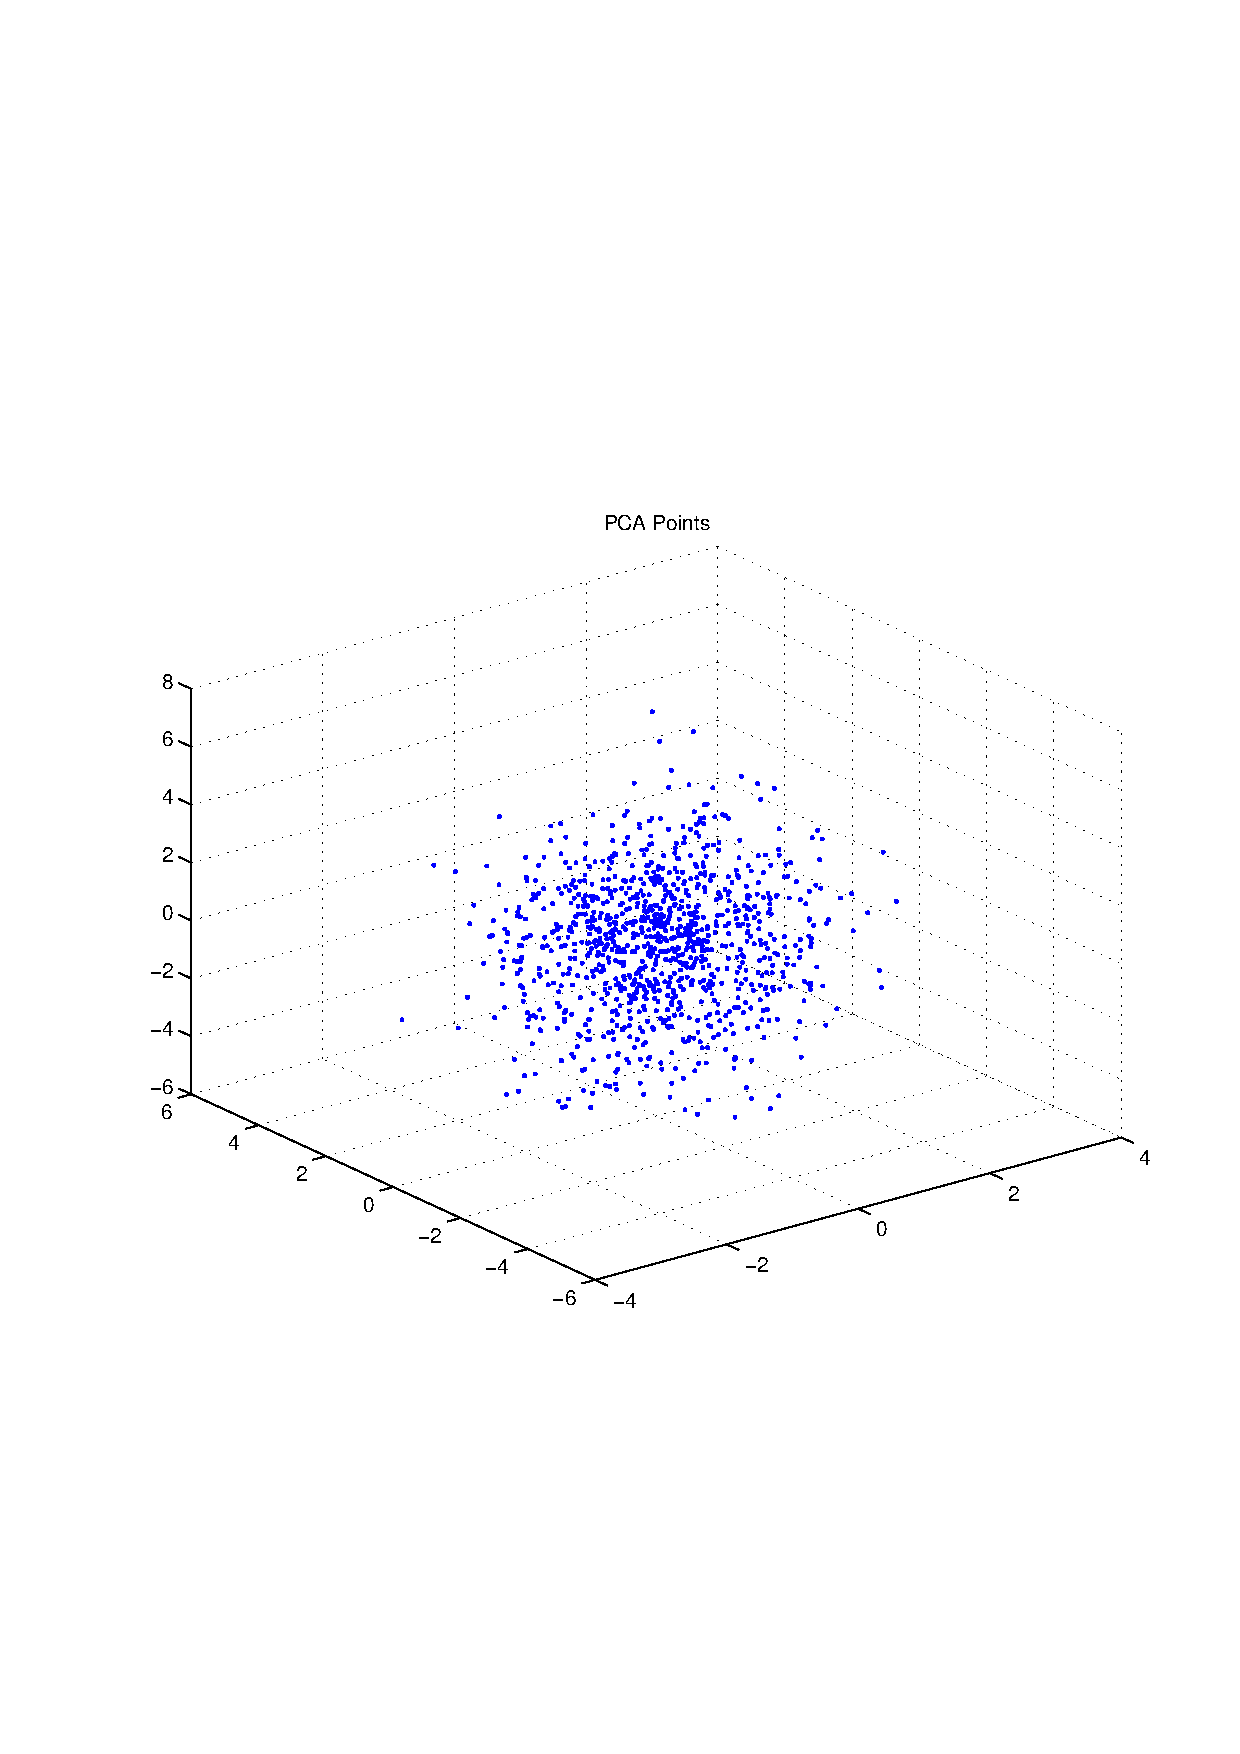
\includegraphics[width=10.0cm,height=10.0cm]{PCAPoints.pdf}

The eigenvectors:
+0.086, +0.286, +0.954
+0.185, +0.937, -0.297
-0.979, +0.203, +0.028

All of the eigenvalues of the covariance matrix:
(+0.958,+0.000), (+2.025,+0.000), (+3.017,+0.000)

QueryPerformanceCounter  =  +1.063
\subsubsection{Multi Variate Random Number Generator }
Sample from $N(\mu,\Sigma)$
mean= -0.002, variance=+1.004, skewness=+0.006, kurtosis=+3.003
mean= -0.001, variance=+1.017, skewness=-0.005, kurtosis=+2.988
mean= -0.002, variance=+1.006, skewness=-0.016, kurtosis=+3.014
Covariance Matrix 
+1.004, +0.009, +0.003
+0.009, +1.017, -0.003
+0.003, -0.003, +1.006

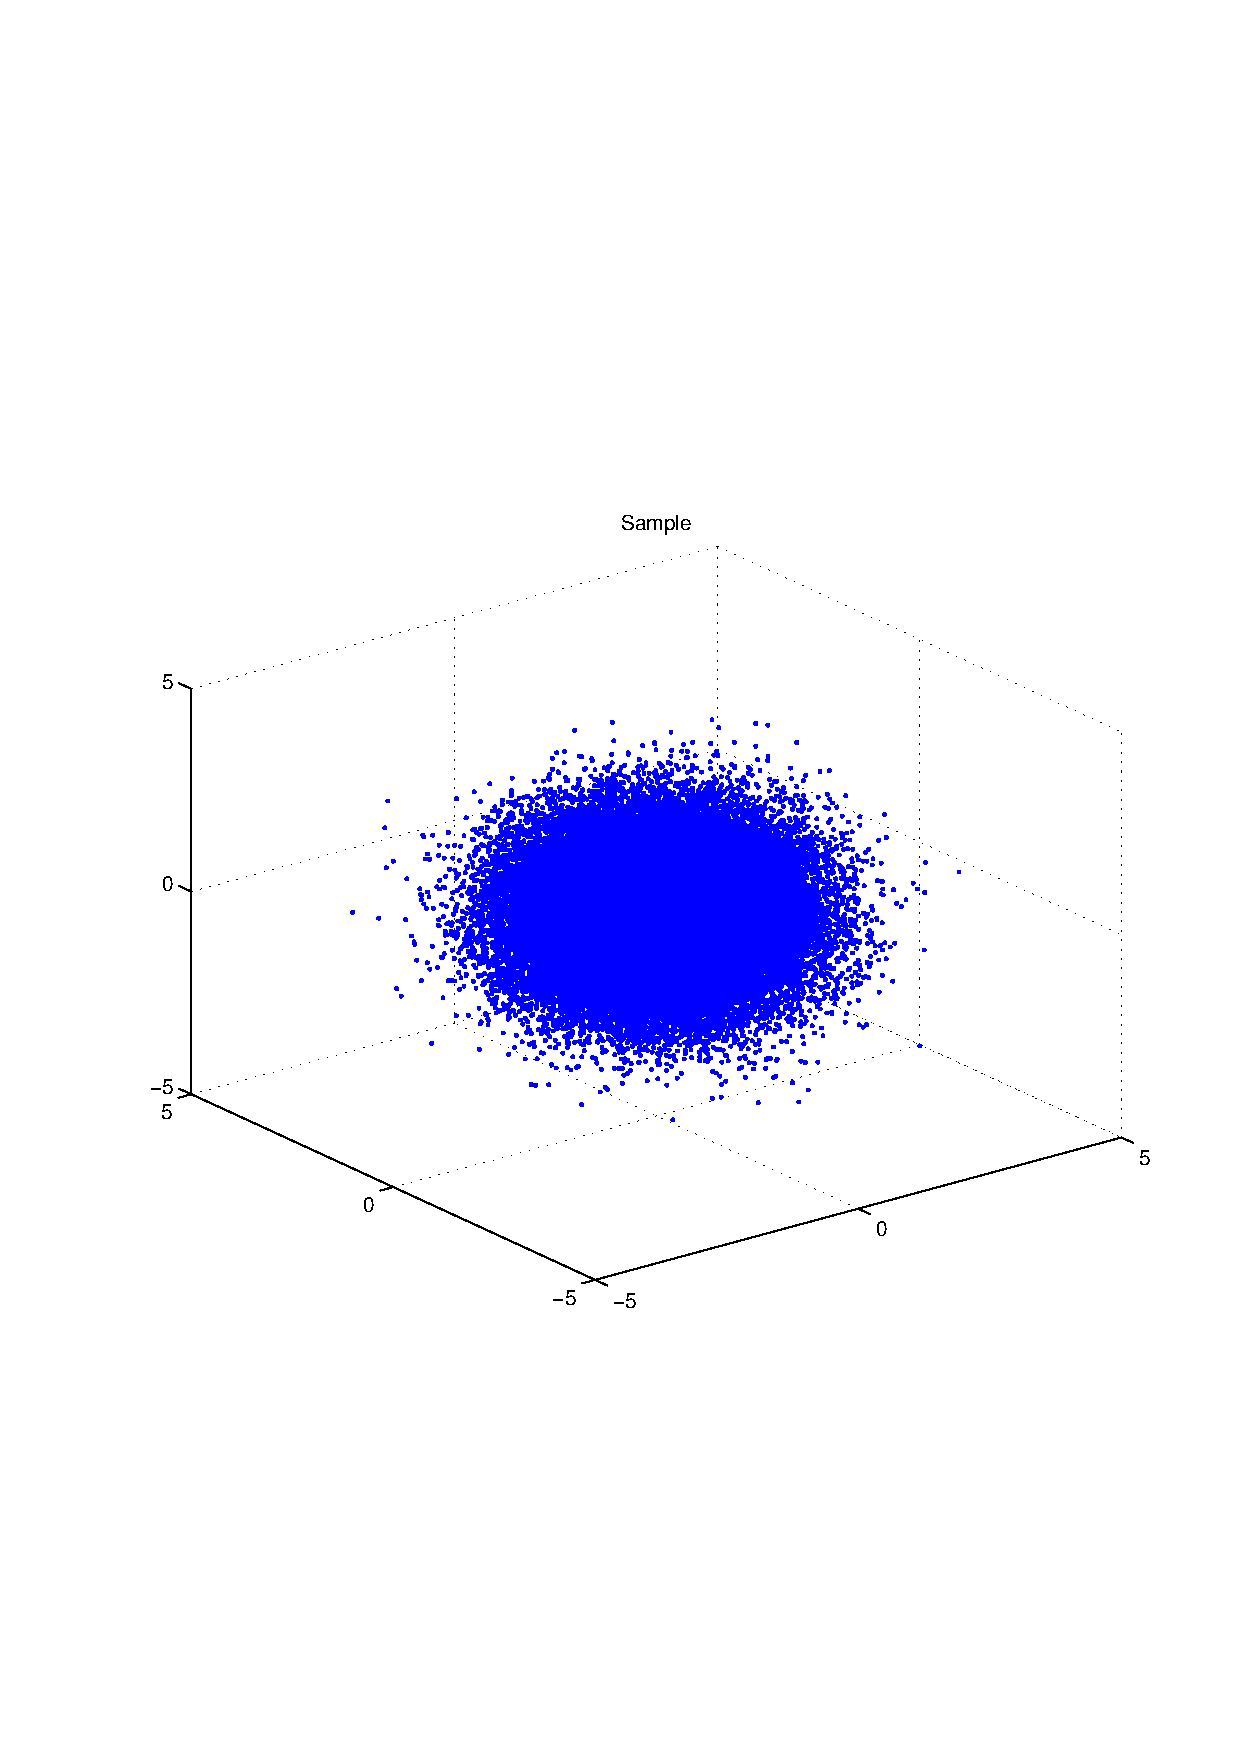
\includegraphics[width=10.0cm,height=10.0cm]{R_3_Normal.pdf}

Generate a sample from a unifom mixture of three Gaussians in $R^3$
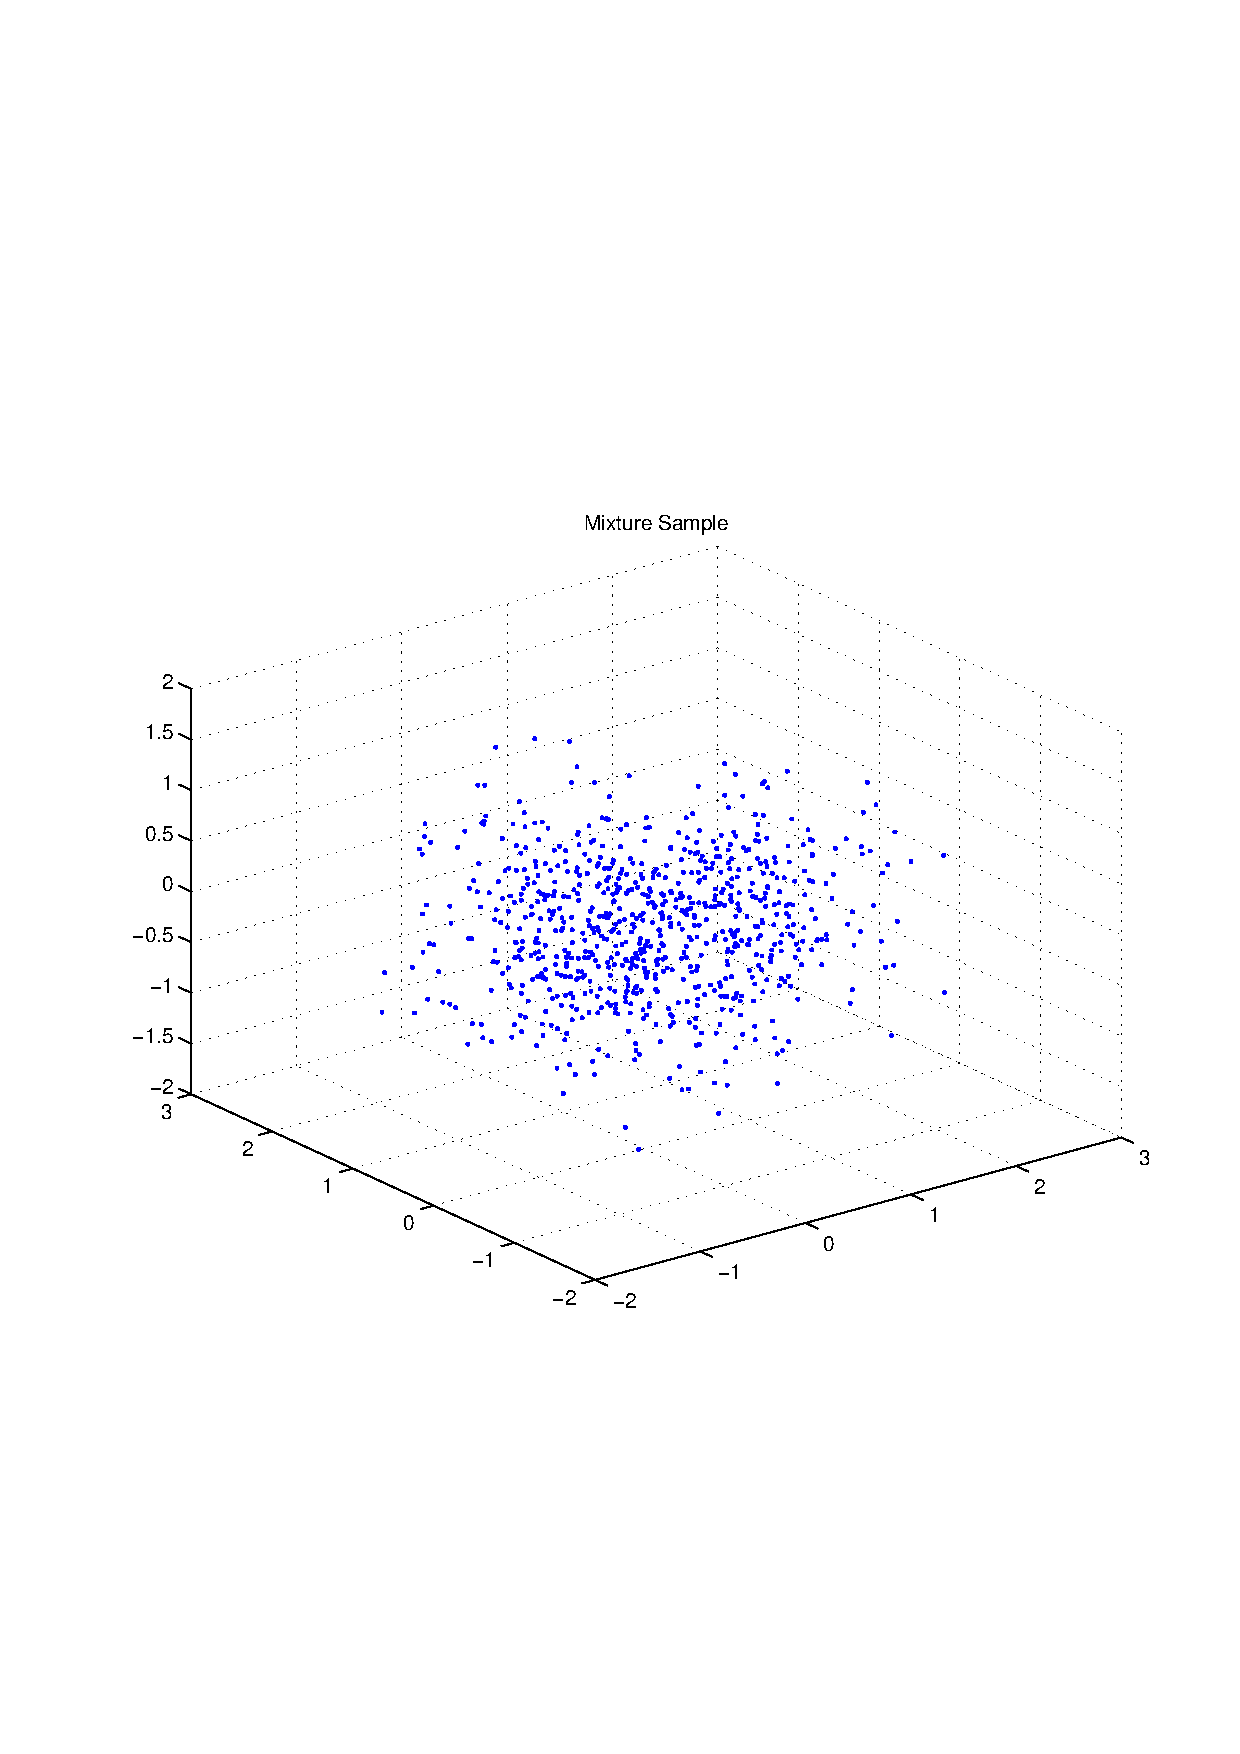
\includegraphics[width=10.0cm,height=10.0cm]{R_3_Normal_Mixture.pdf}

QueryPerformanceCounter  =  +16.620
\subsubsection{Matrix Multiply}
Comparing naive matrix multiply verus Intel MKL dgemm for matrix of size +2048.
This is for type double (hence the d in dgemm).
Naive type double matrix multiply tic toc  =  +0.348
dgemm plus row to column major transpose operation tic toc  =  +0.306
Comparing naive matrix multiply verus Intel MKL sgemm for matrix of size +2048.
This is for type float (hence the s in dgemm).
Naive type float matrix multiply tic toc  =  +0.223
sgemm plus row to column major transpose operation tic toc  =  +0.202
QueryPerformanceCounter  =  +1.198
\subsubsection{Descriptive Statistics}
Mean N(0,1): +0.003
Variance N(0,1): +1.006
Mean N(0,1) [recurrence relation method] :+0.003
Variance [recurrence relation method] :+1.006
Skewness : +0.007
Kurtosis : +2.997
QueryPerformanceCounter  =  +0.019
\subsubsection{Time Series }
+0.093
+0.726
+0.011
+2.178
QueryPerformanceCounter  =  +0.033
QueryPerformanceCounter  =  +6.295
\subsubsection{Iterated Exponential Filtering }
$\mu_1 =+0.093$
$\mu_2 =+0.726$
$\mu_3 =+0.011$
$\mu_4 =+2.178$
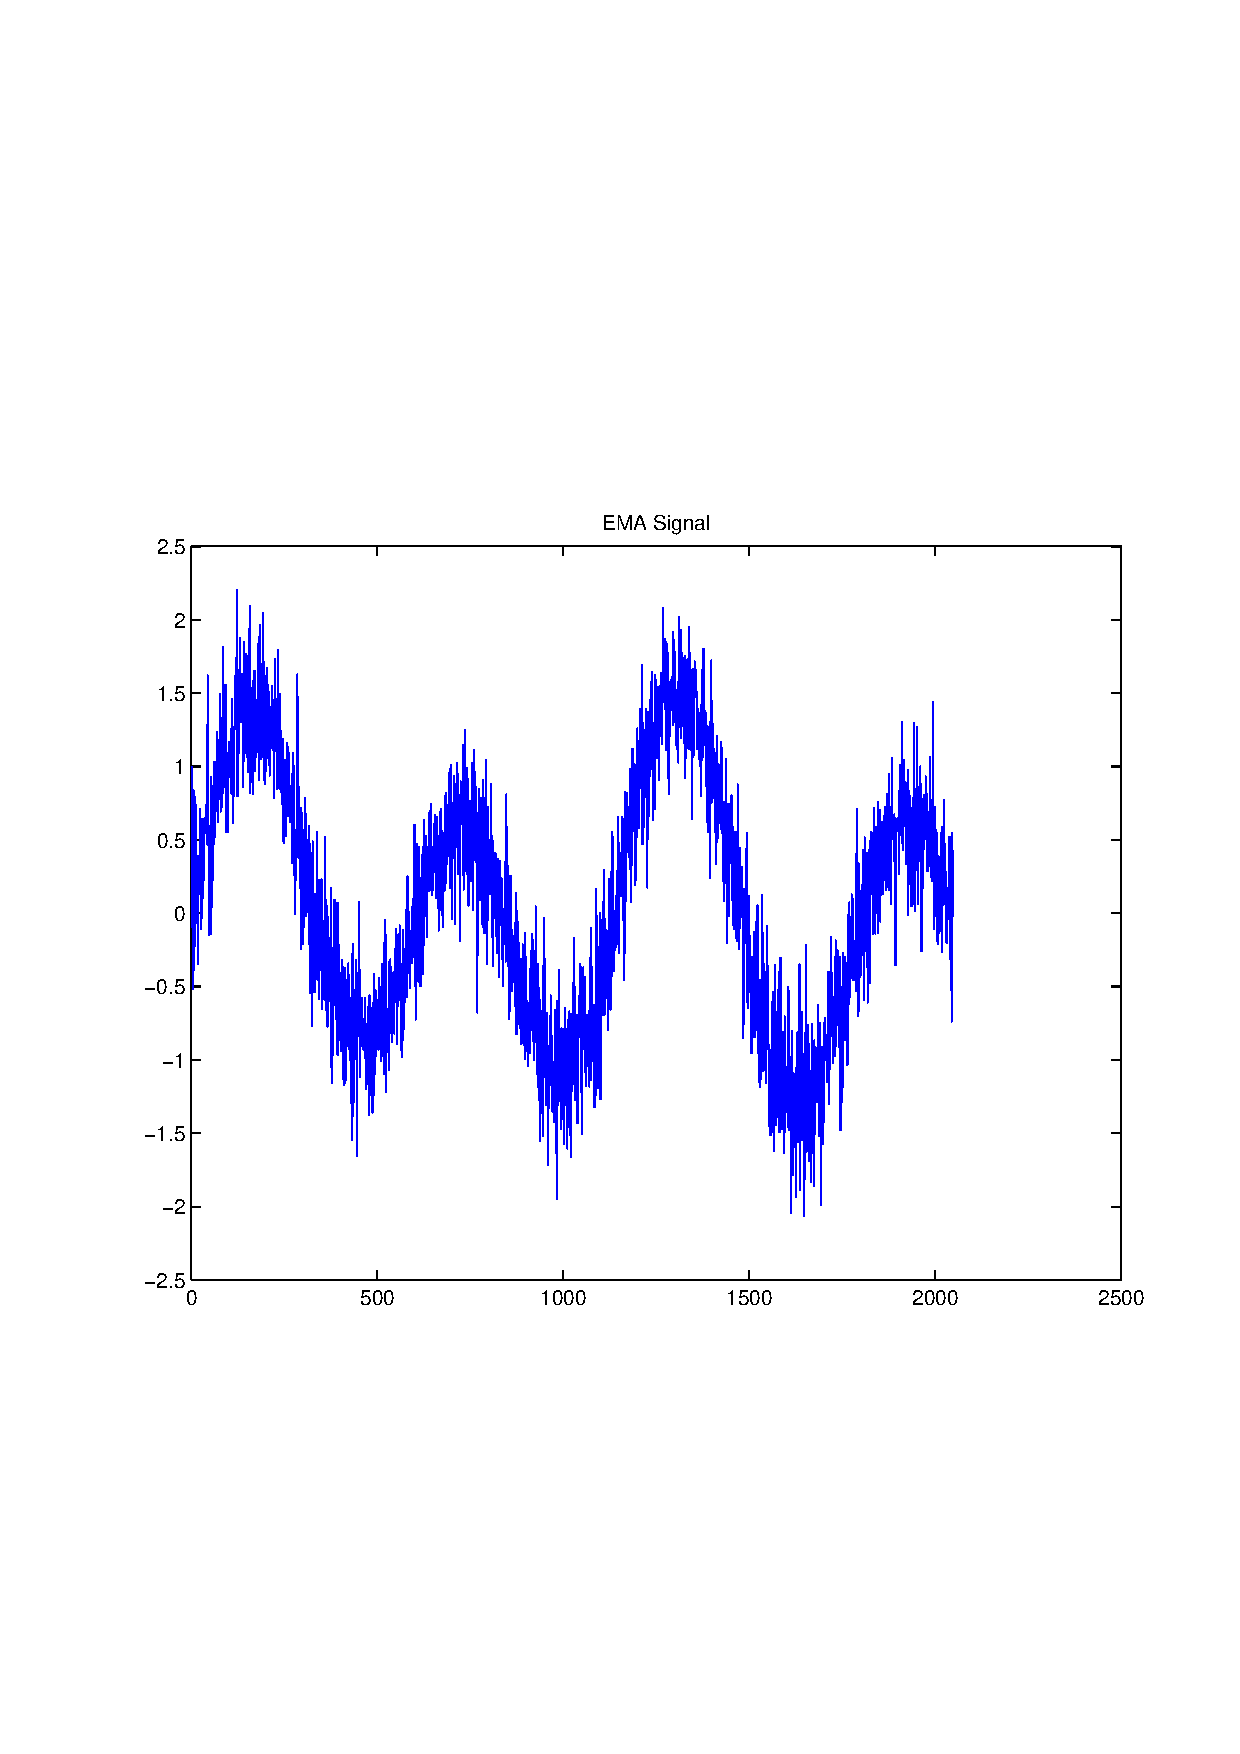
\includegraphics[width=10.0cm,height=10.0cm]{EMA_signal.pdf}

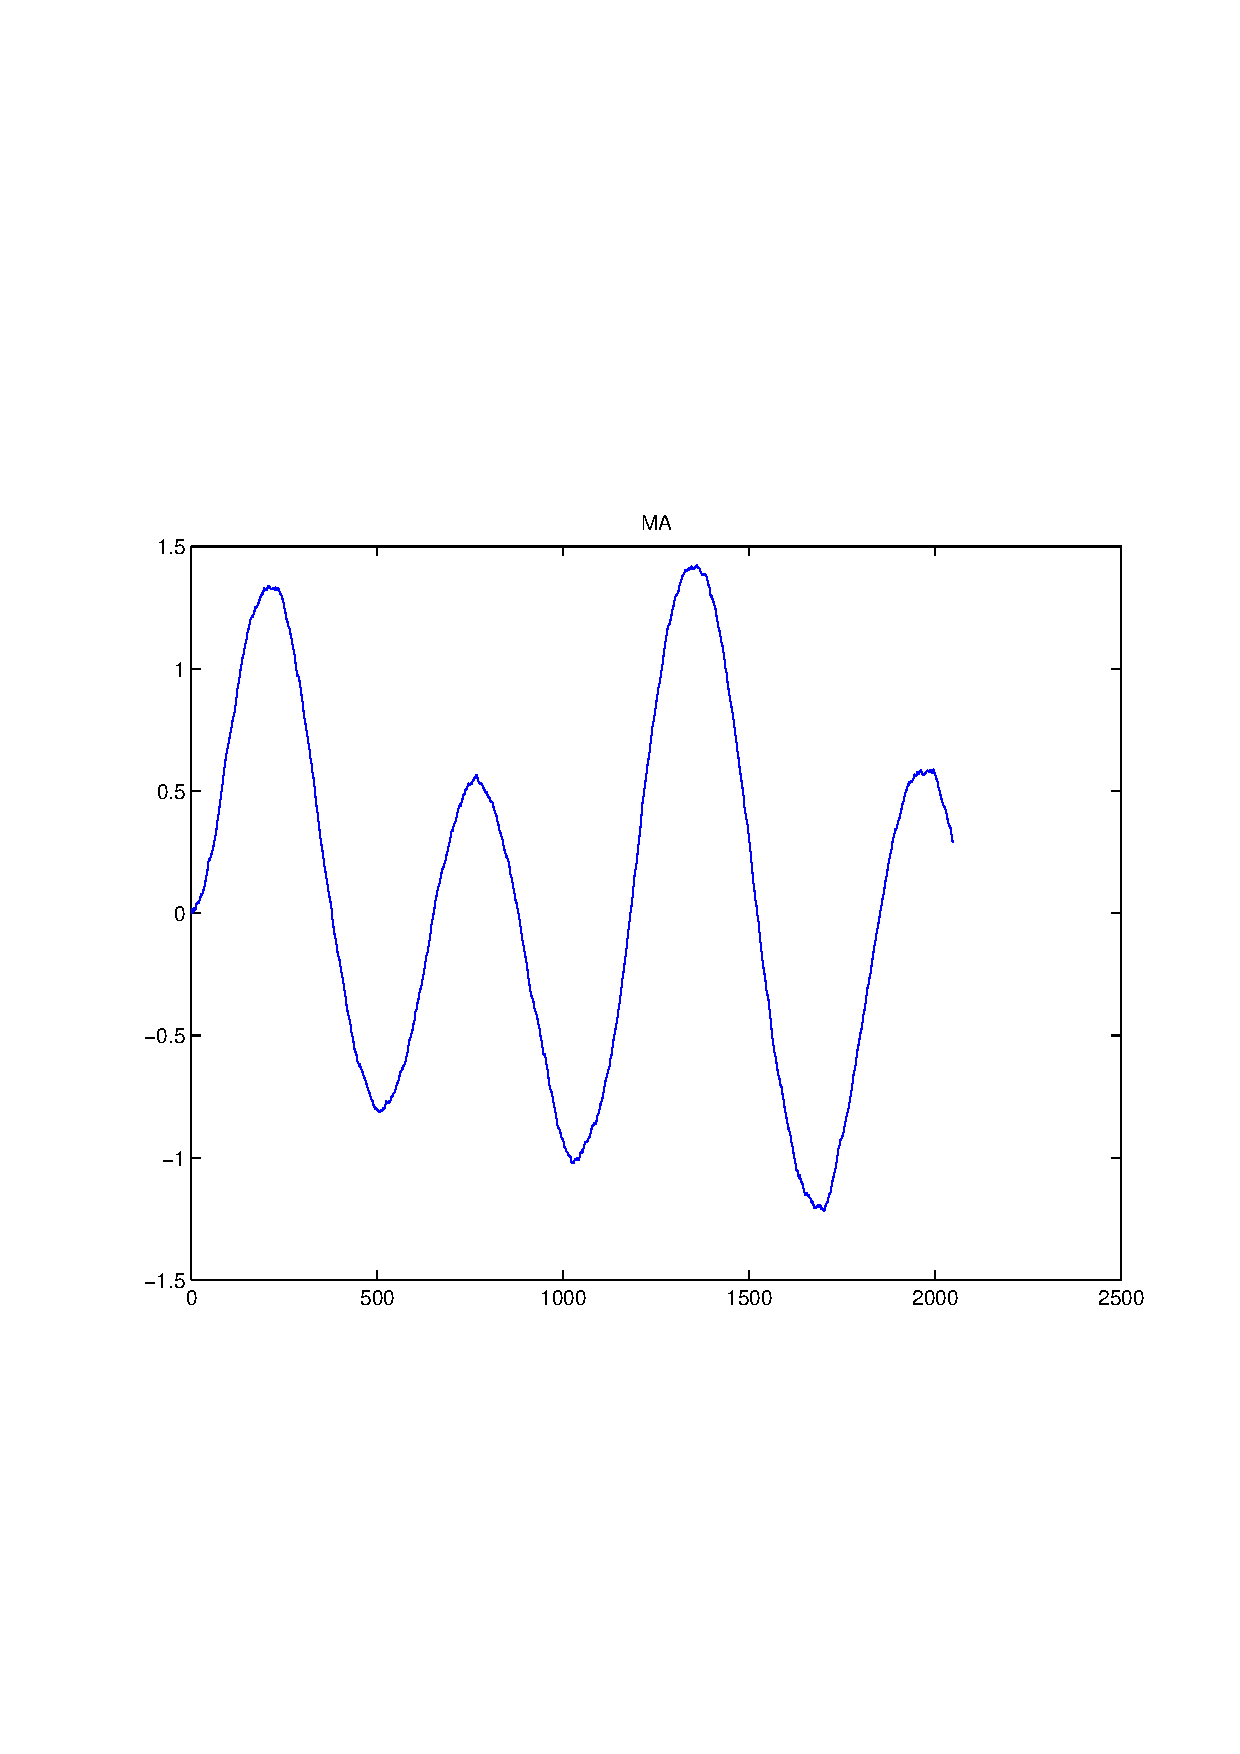
\includegraphics[width=10.0cm,height=10.0cm]{MA.pdf}

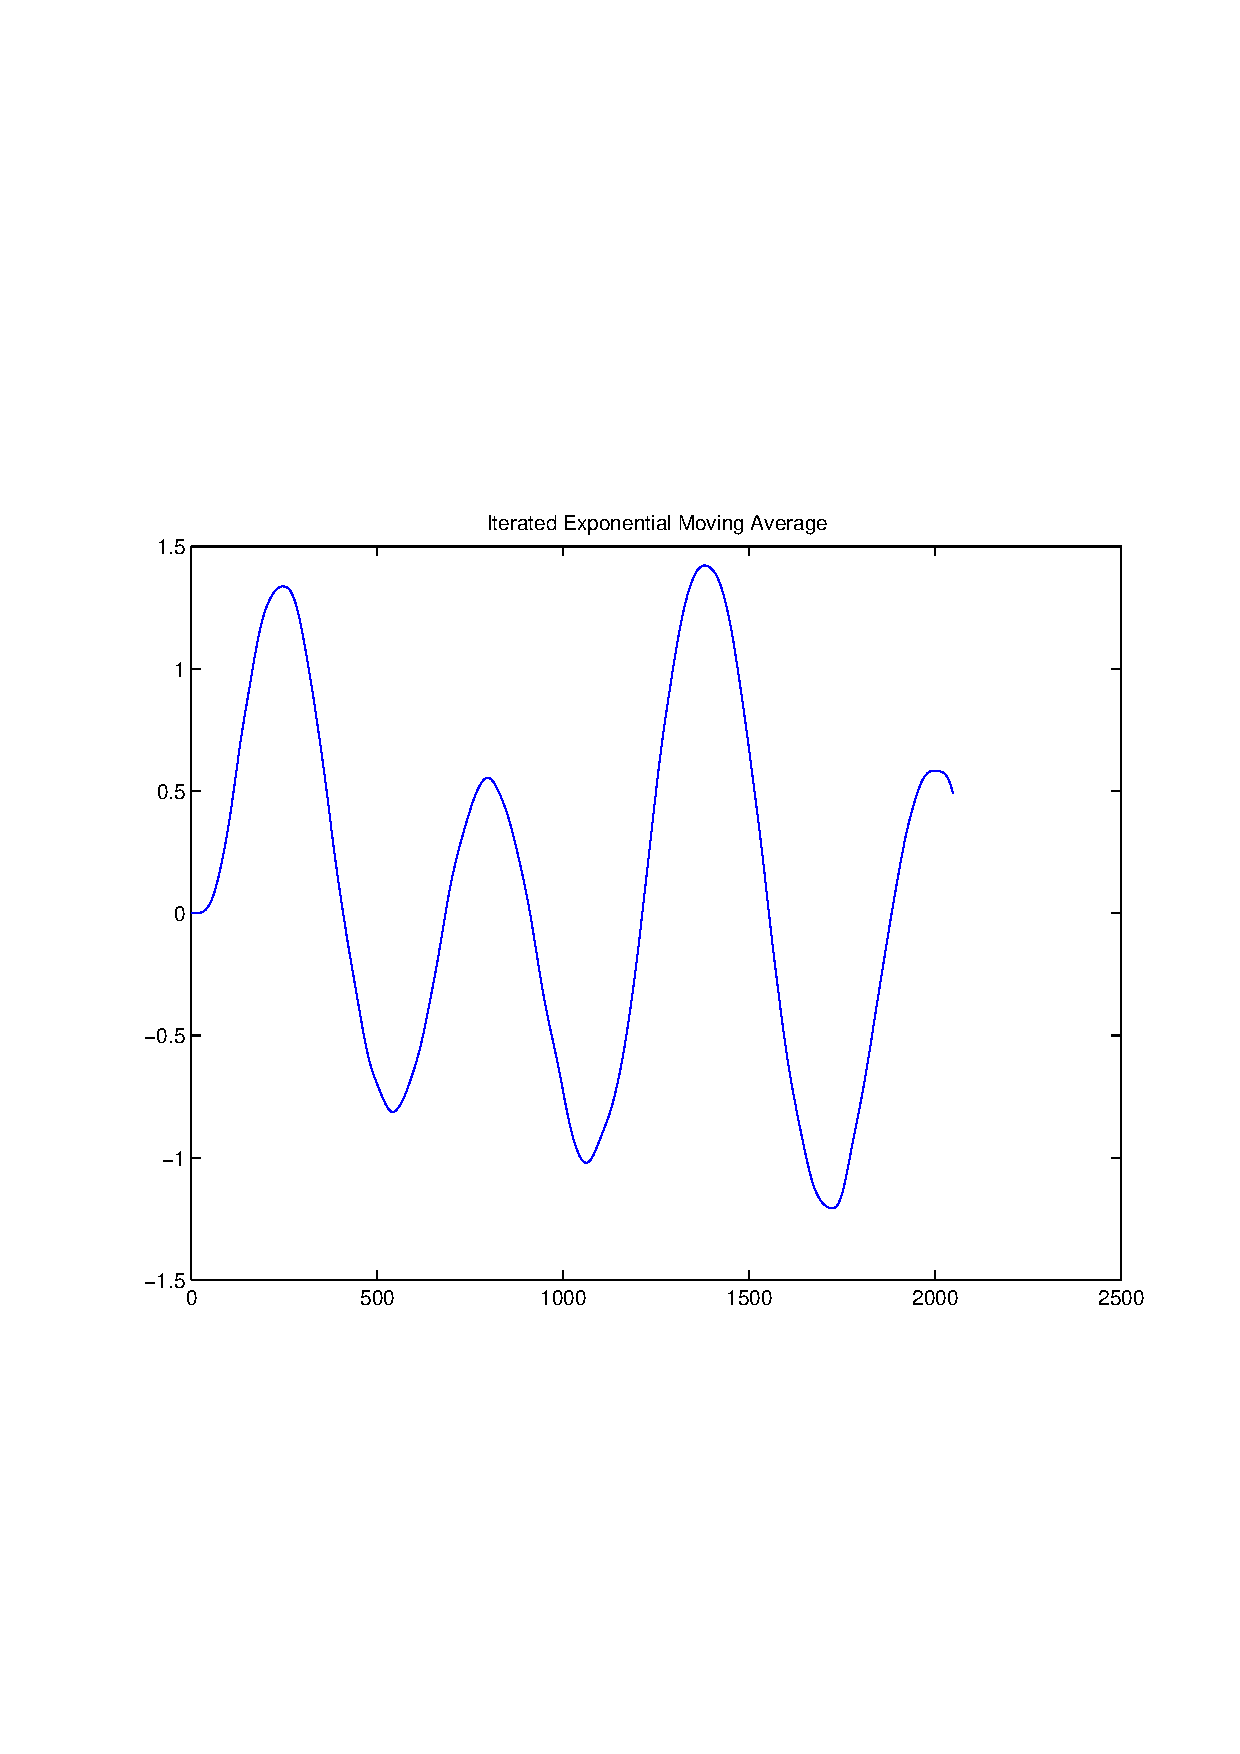
\includegraphics[width=10.0cm,height=10.0cm]{IEMA.pdf}

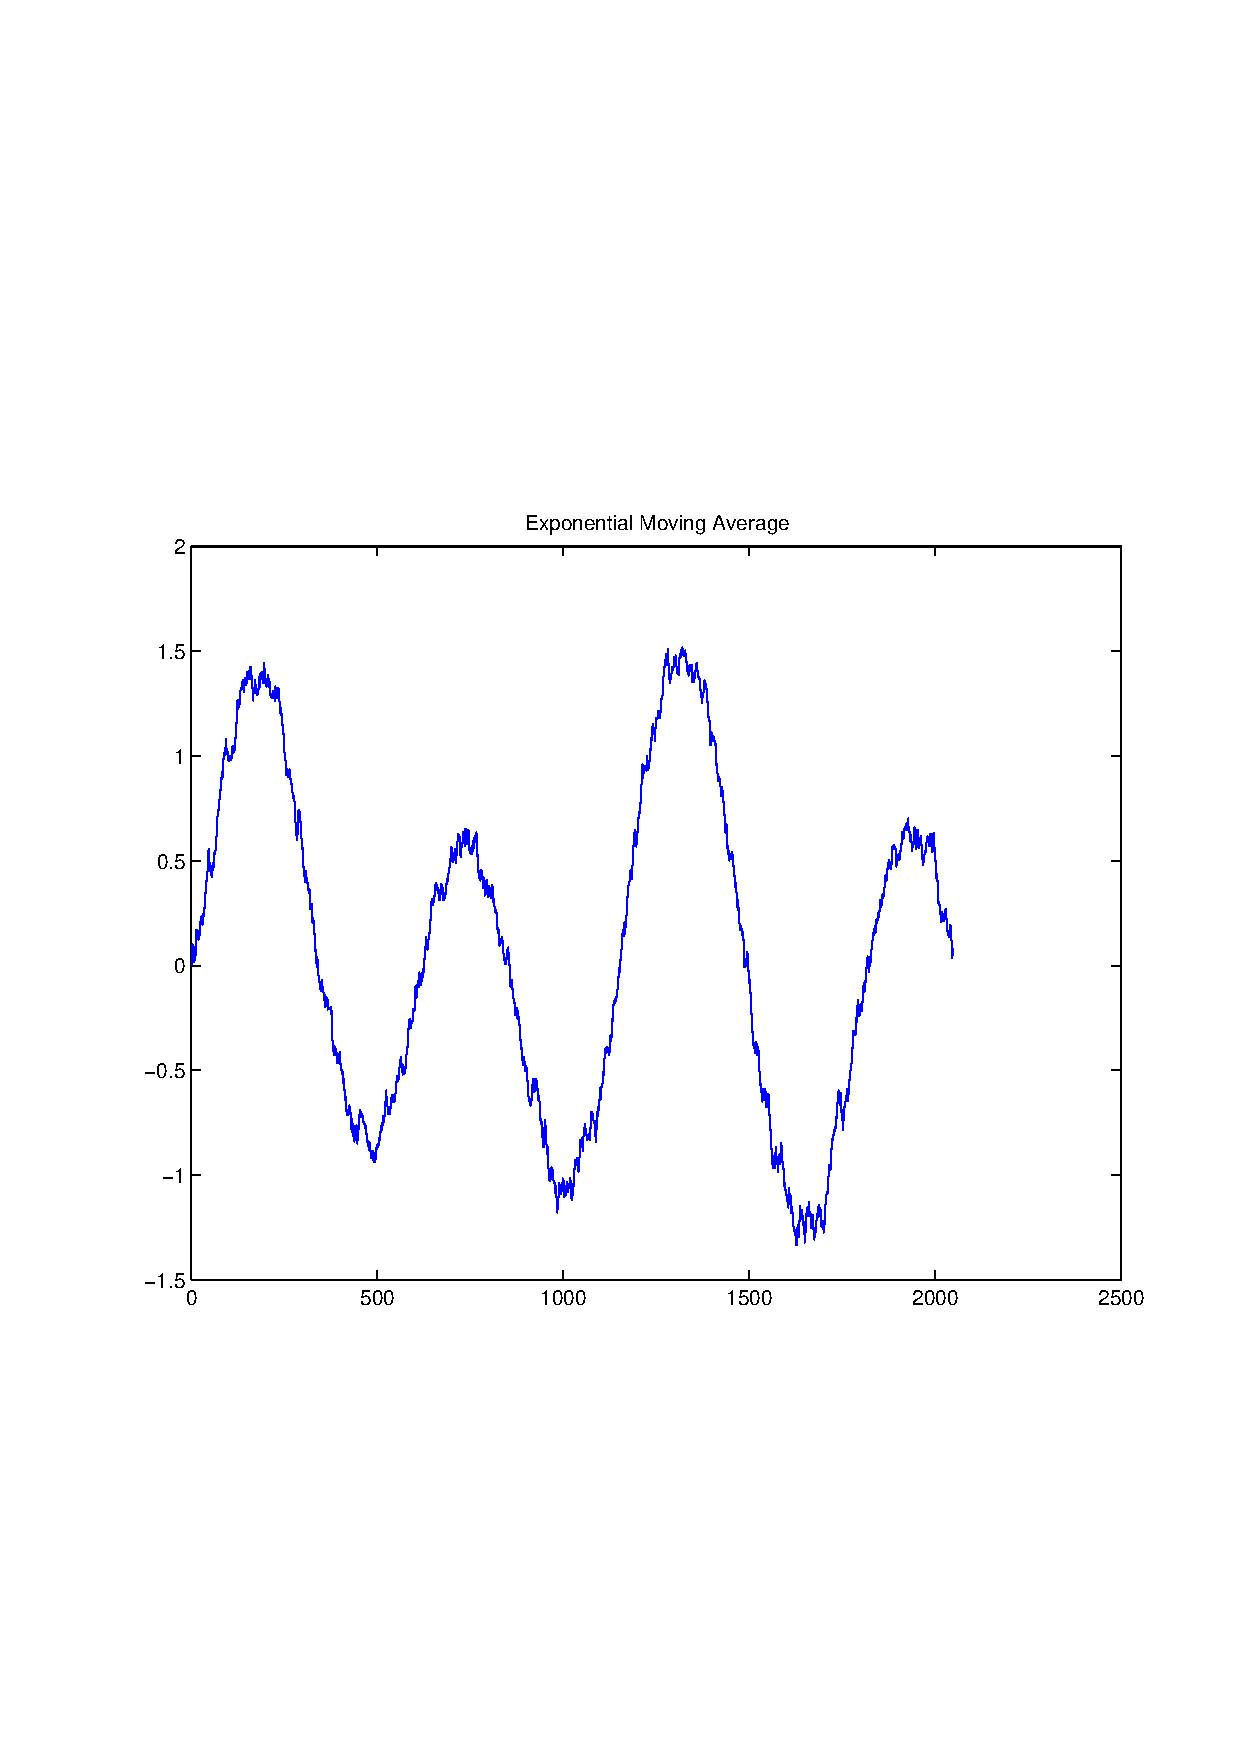
\includegraphics[width=10.0cm,height=10.0cm]{EMA.pdf}

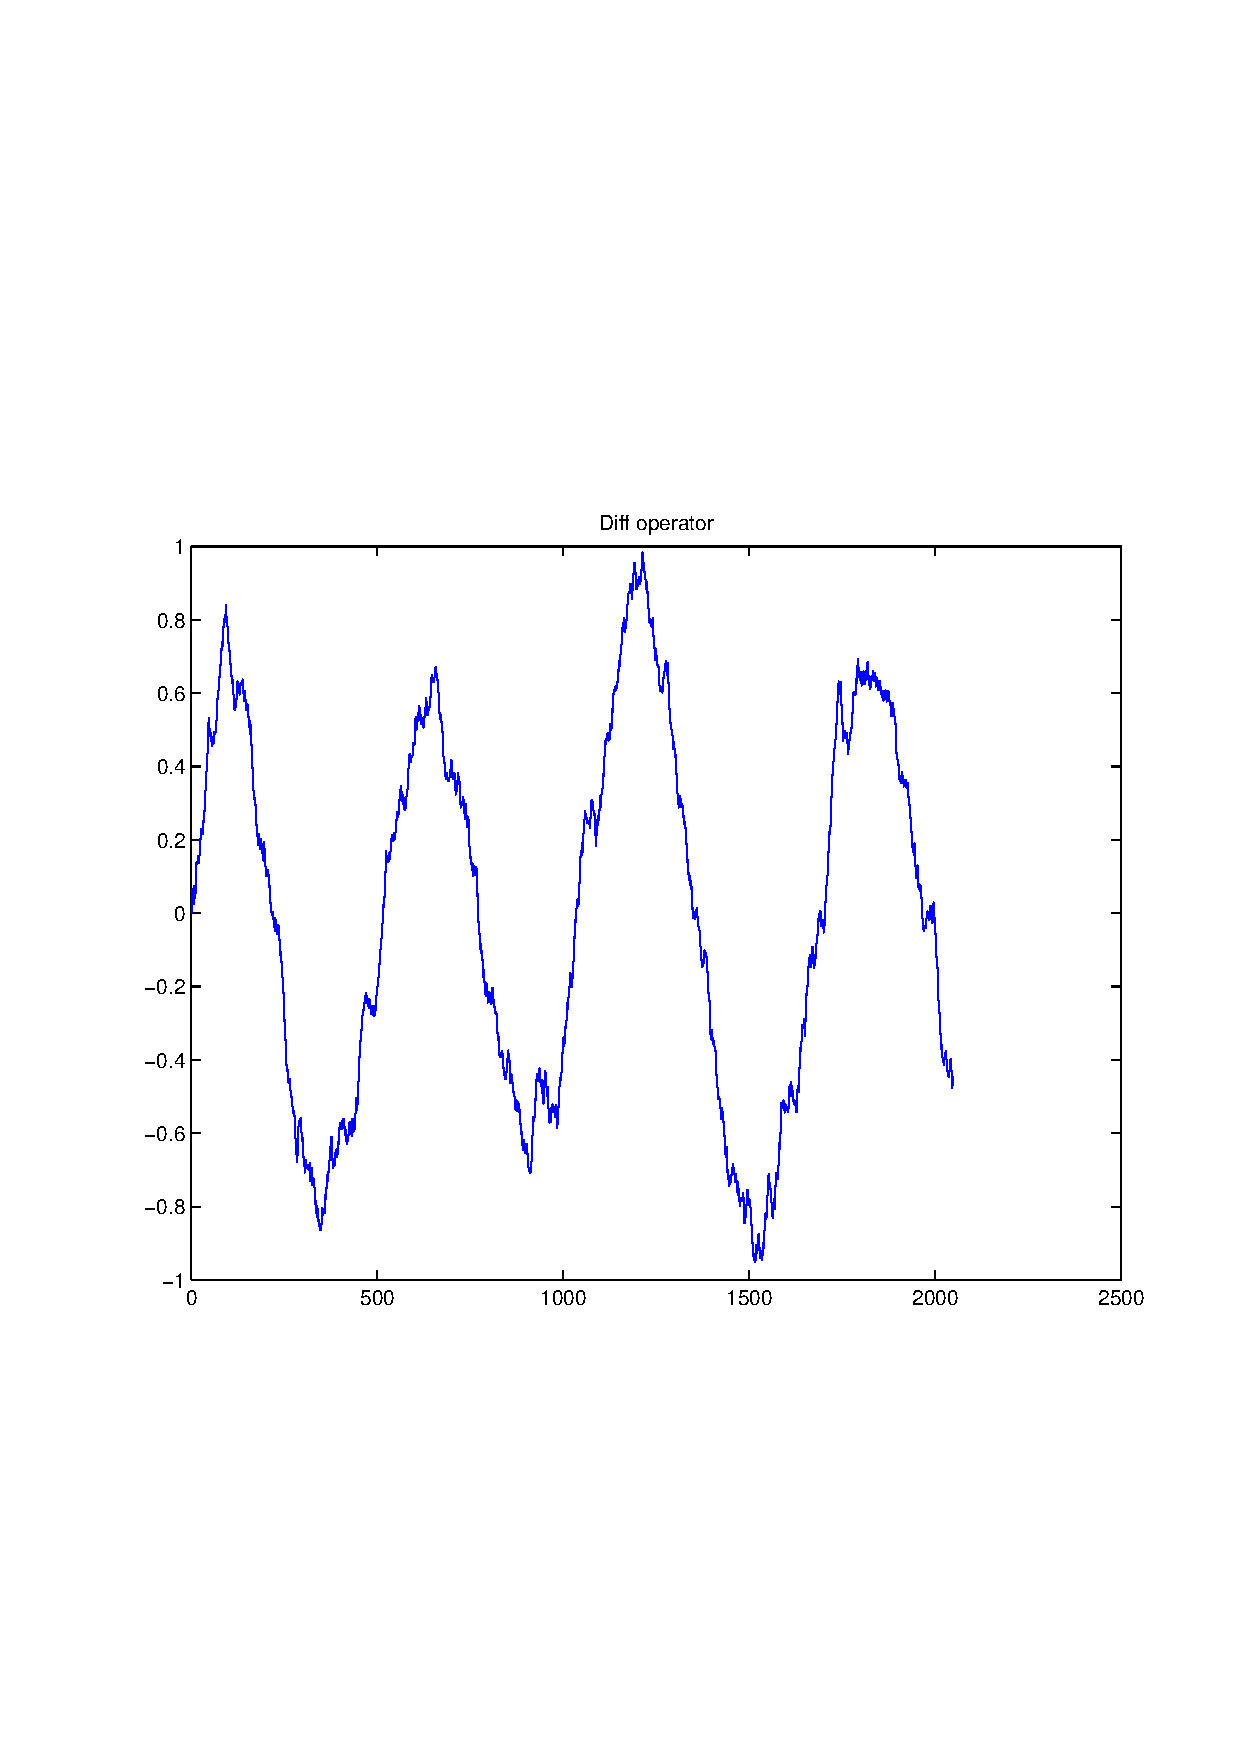
\includegraphics[width=10.0cm,height=10.0cm]{DIFF.pdf}

\includegraphics[width=10.0cm,height=10.0cm]{IteratedExponentailOperators.pdf}

\includegraphics[width=10.0cm,height=10.0cm]{IteratedExponentailOperators.pdf}

QueryPerformanceCounter  =  +7.850
\subsubsection{Testing binary writer}
Binary writer Speedup 1GB Double Matrix +52.148

Binary reader Speedup 1GB Double Matrix +194.730

Binary writer Speedup 1GB Double vector +47.365

Binary reader Speedup 1GB Double Matrix +165.990

QueryPerformanceCounter  =  +0.903
\subsubsection{Testing Gaussian Mixture Point Cloud and Latex Plotting Capabilities.}
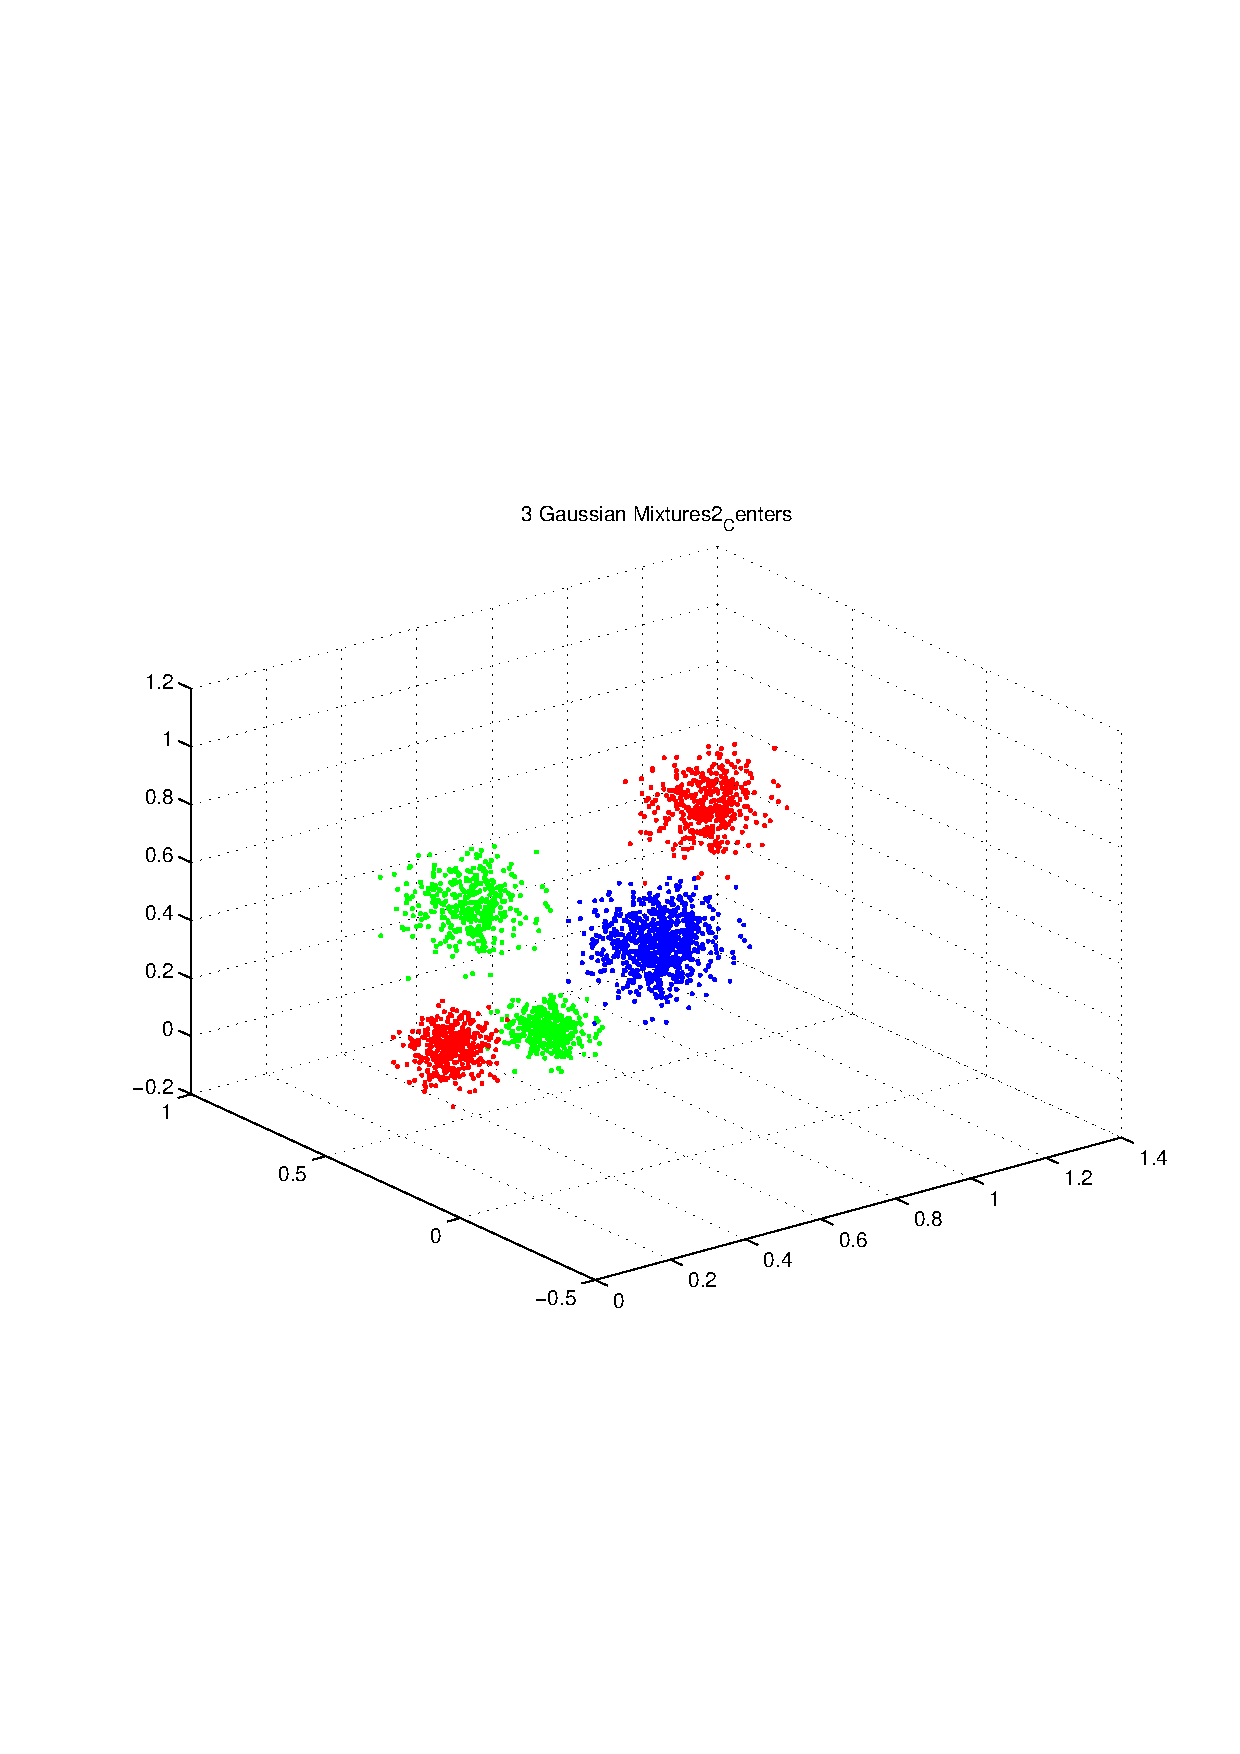
\includegraphics[width=10.0cm,height=10.0cm]{GaussianMixture_Dim_3_Centers2.pdf}

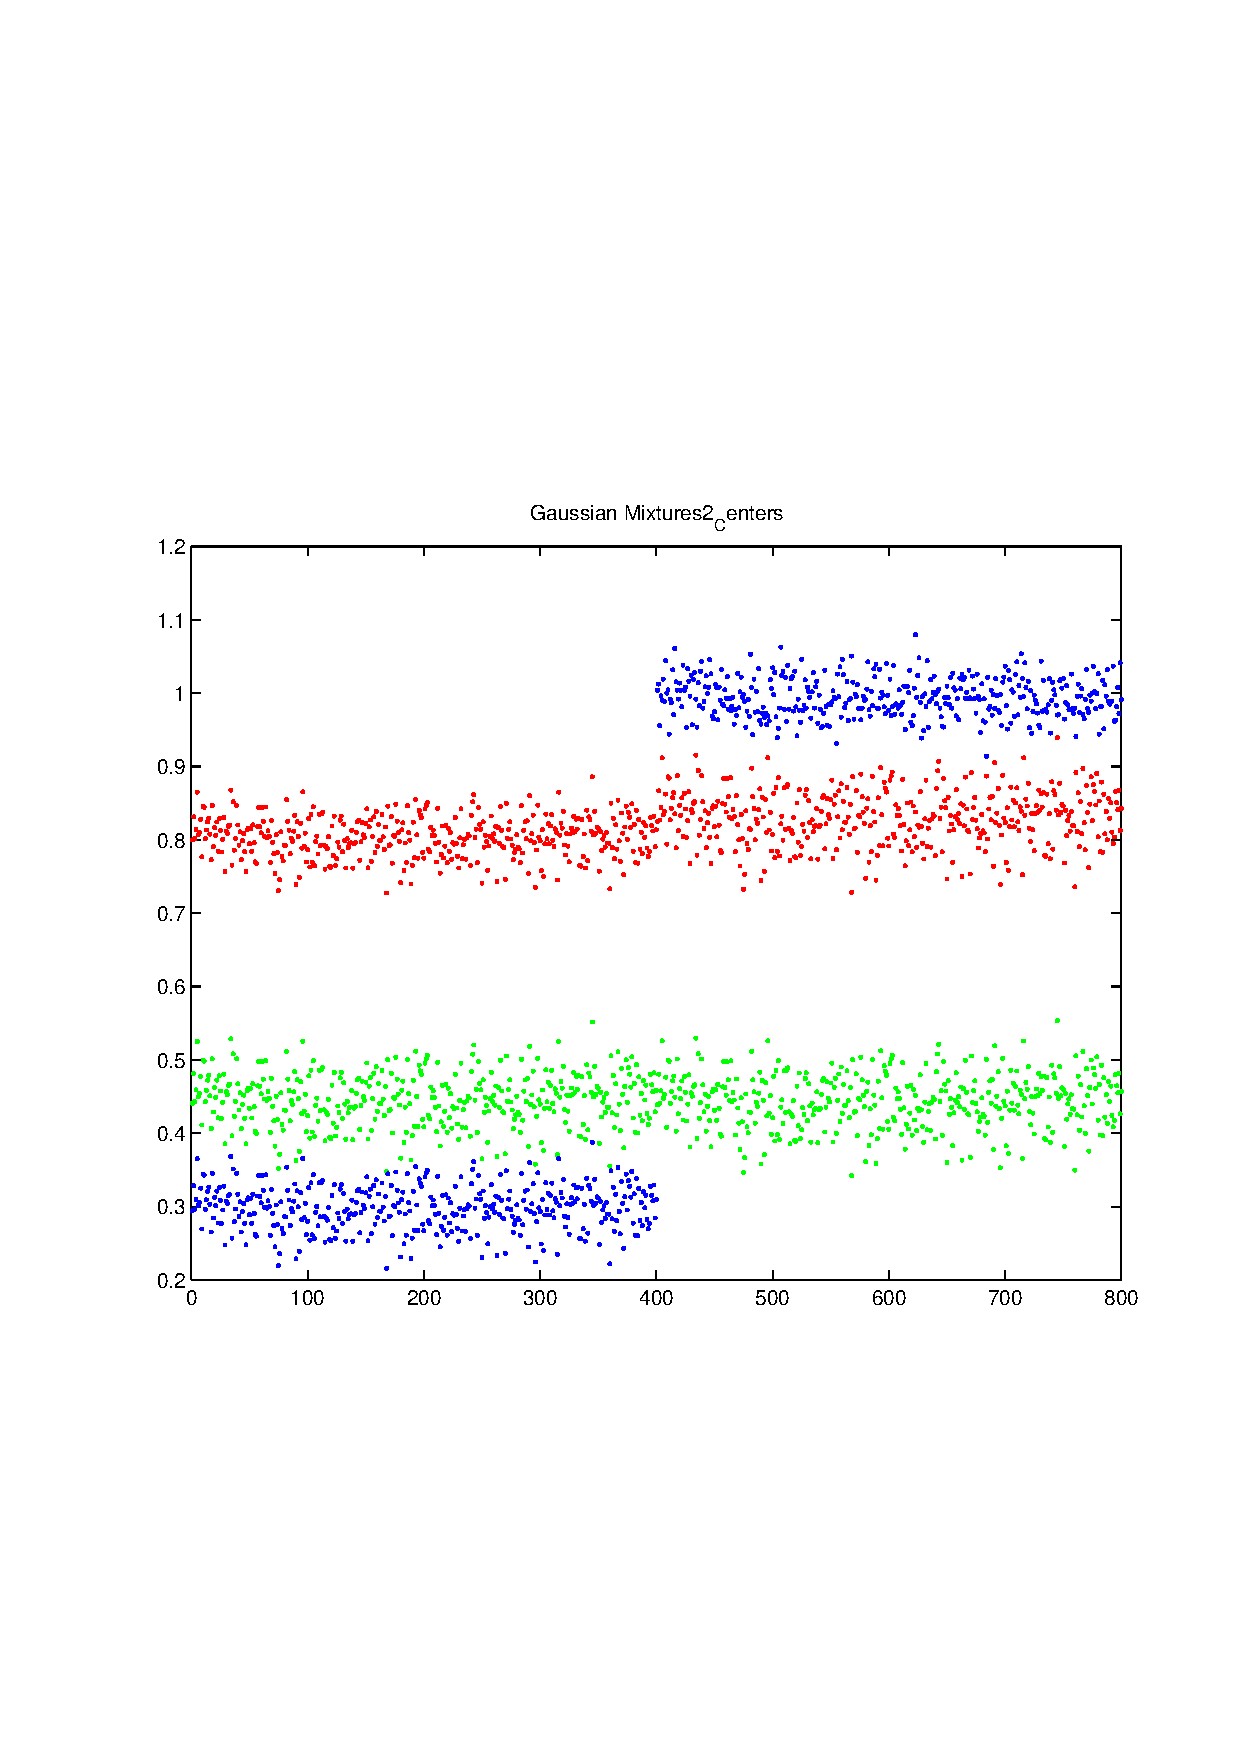
\includegraphics[width=10.0cm,height=10.0cm]{GaussianMixture_Dim_1_Centers2.pdf}

QueryPerformanceCounter  =  +2.806
\subsubsection{Intel VSL Function Check}
\includegraphics[width=10.0cm,height=10.0cm]{klVSLInv.pdf}

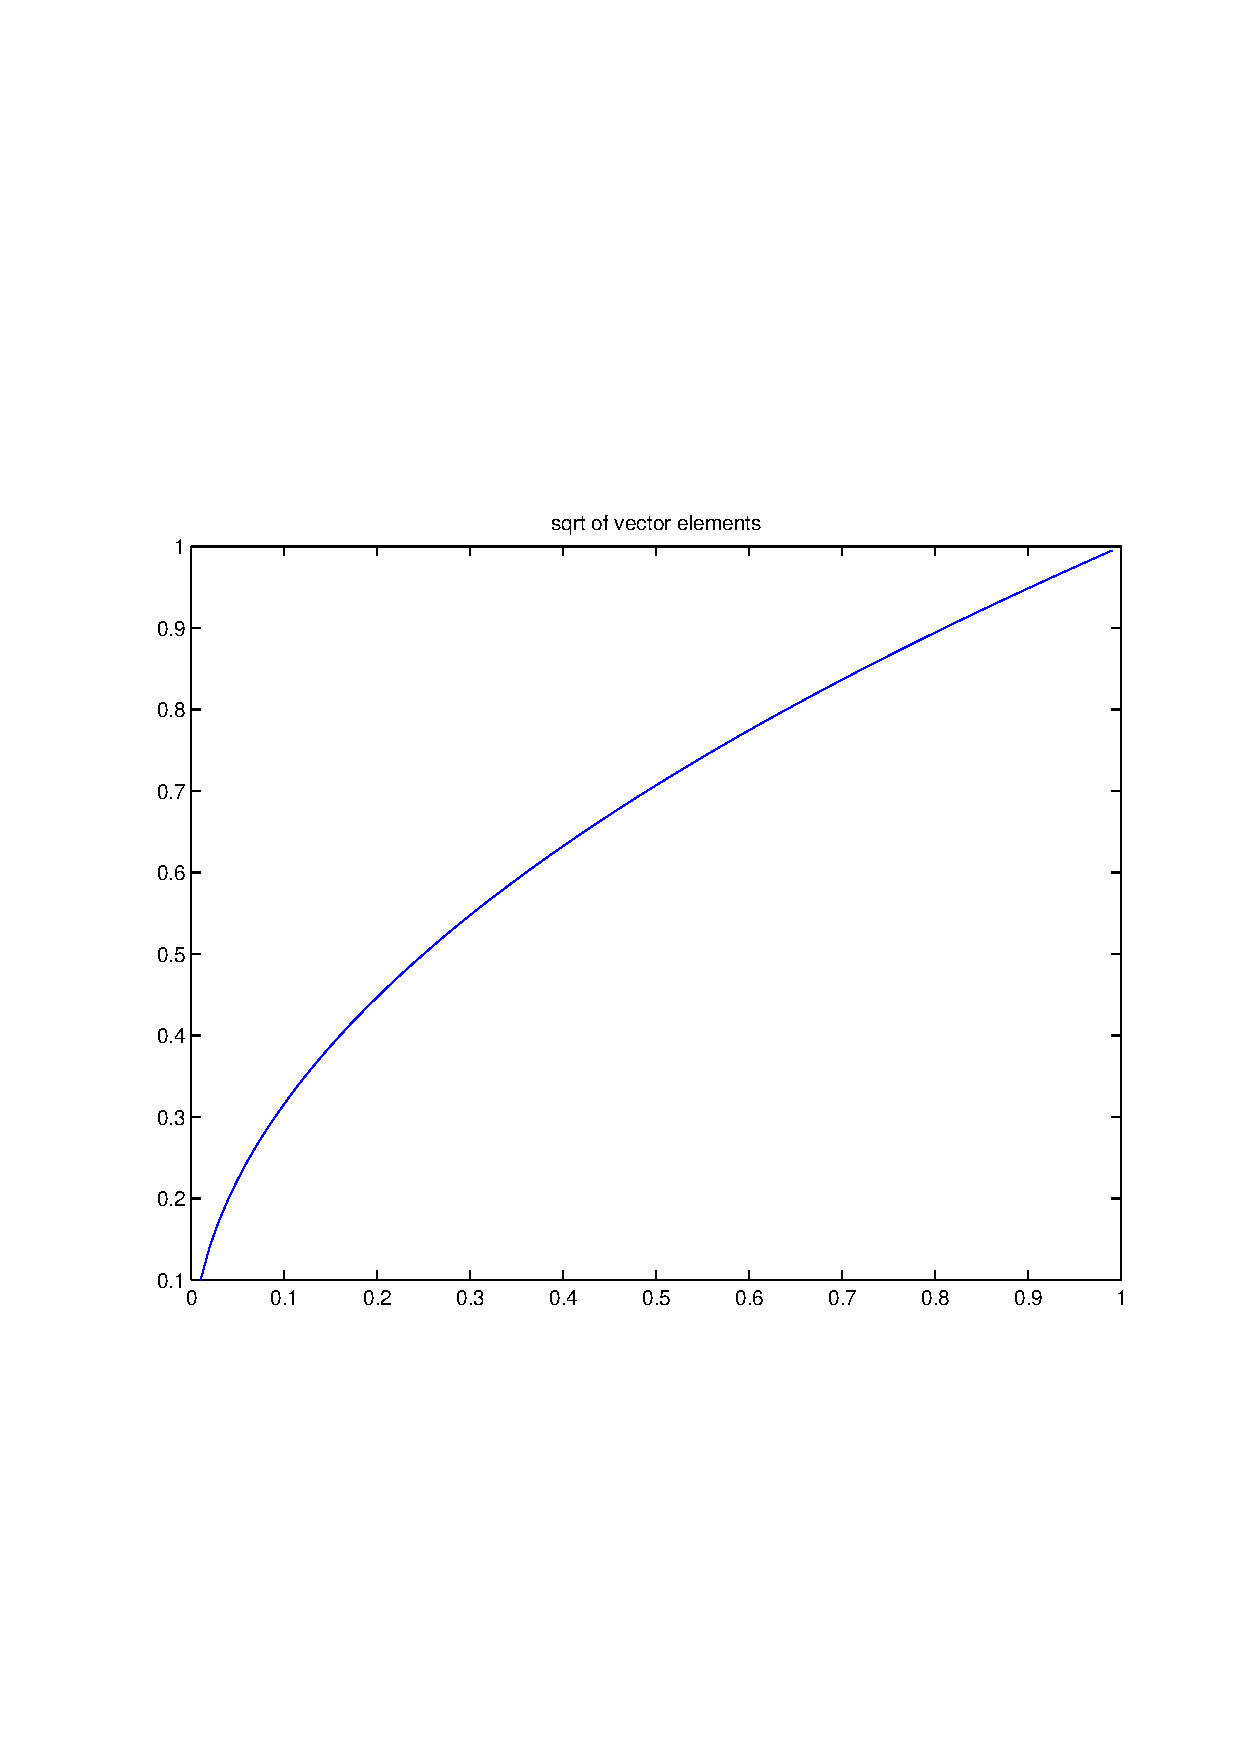
\includegraphics[width=10.0cm,height=10.0cm]{klVSLSqrt.pdf}

\includegraphics[width=10.0cm,height=10.0cm]{klVSLExp.pdf}

\includegraphics[width=10.0cm,height=10.0cm]{klVSLExpm1.pdf}

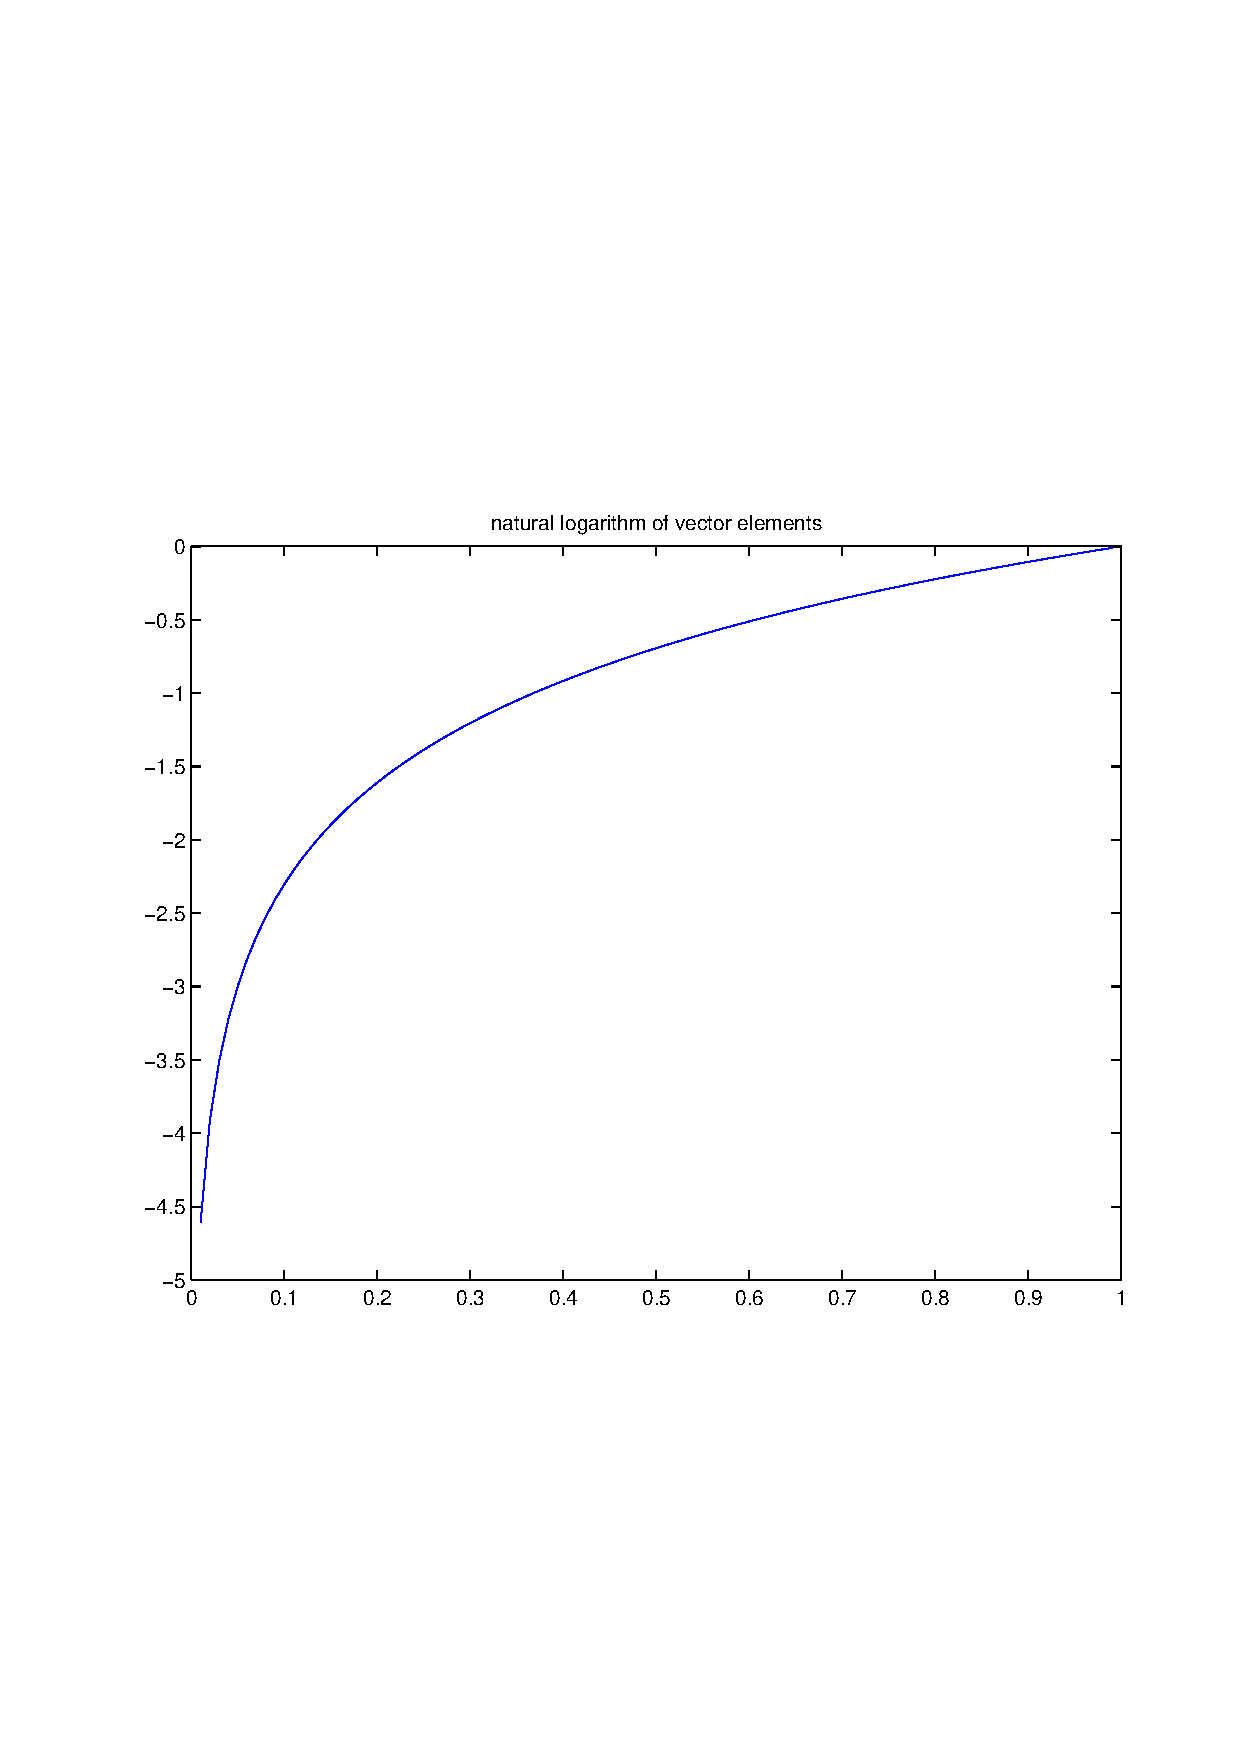
\includegraphics[width=10.0cm,height=10.0cm]{klVSLLn.pdf}

\includegraphics[width=10.0cm,height=10.0cm]{klVSLLog10.pdf}

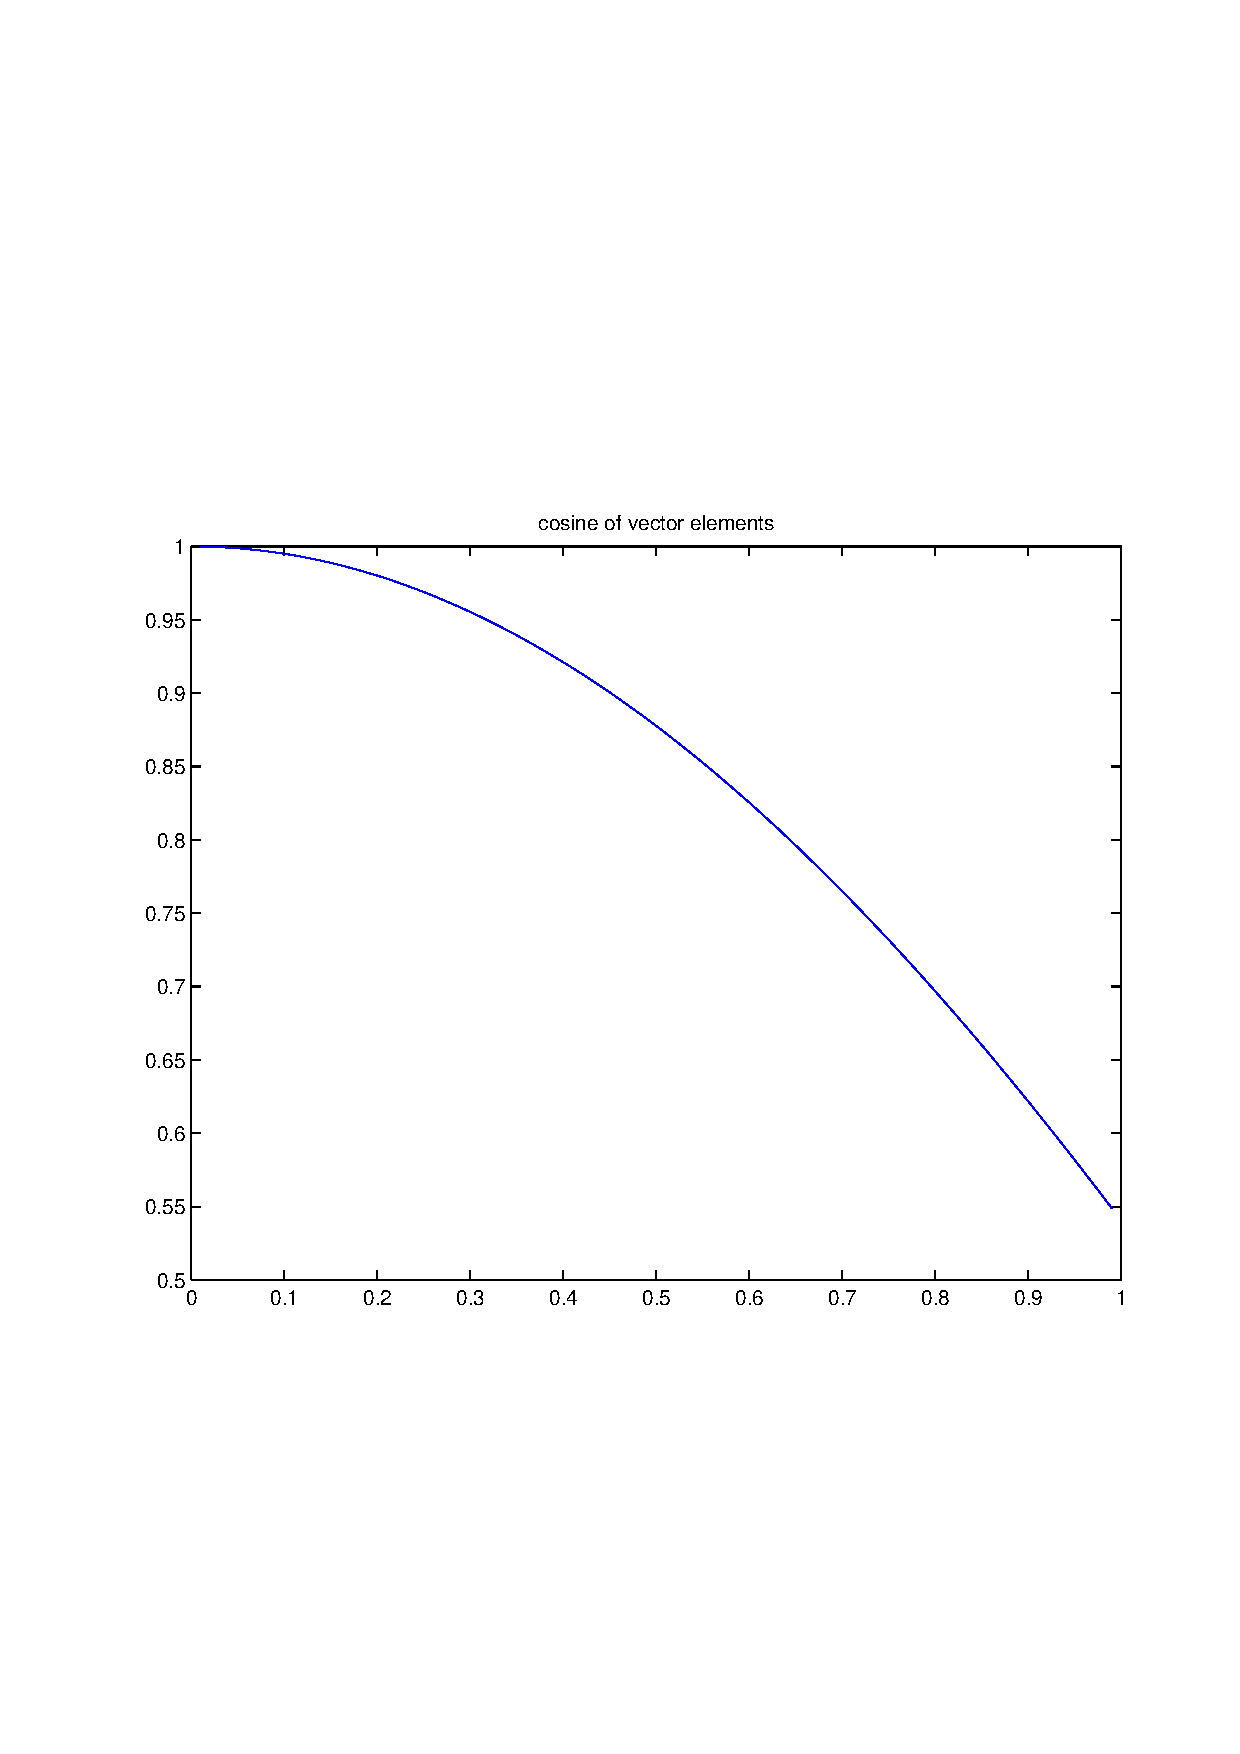
\includegraphics[width=10.0cm,height=10.0cm]{klVSLCos.pdf}

\includegraphics[width=10.0cm,height=10.0cm]{klVSLSin.pdf}

\includegraphics[width=10.0cm,height=10.0cm]{klVSLTan.pdf}

\includegraphics[width=10.0cm,height=10.0cm]{klVSLErf.pdf}

\includegraphics[width=10.0cm,height=10.0cm]{klVSLErfc.pdf}

\includegraphics[width=10.0cm,height=10.0cm]{klVSLCdfNorm.pdf}

\includegraphics[width=10.0cm,height=10.0cm]{klVSLErfInv.pdf}

\includegraphics[width=10.0cm,height=10.0cm]{klVSLLGamma.pdf}

\includegraphics[width=10.0cm,height=10.0cm]{klVSLTGamma.pdf}

QueryPerformanceCounter  =  +15.228
\subsubsection{Gram Matrix Consistency Check}
Sample Size = 4096
Feature dim = 3

$$Sigma$ = \left(
\begin{array}{
ccc}
+1.140 & +1.535 & +0.581 \\
+1.535 & +9.988 & +1.605 \\
+0.581 & +1.605 & +0.428 \\
\end{array}
\right)$ \newline 

$Sample Covariance = \left(
\begin{array}{
ccc}
+1.152 & +1.538 & +0.584 \\
+1.538 & +10.074 & +1.616 \\
+0.584 & +1.616 & +0.430 \\
\end{array}
\right)$ \newline 

$Sample Mean = \left(
\begin{array}{
ccc}
+1.01364 & +1.00659 & +1.01189 \\
\end{array}
\right)$ \newline 

$Sample Covariance-$Omega$ = \left(
\begin{array}{
ccc}
+0.012 & +0.003 & +0.003 \\
+0.003 & +0.085 & +0.010 \\
+0.003 & +0.010 & +0.002 \\
\end{array}
\right)$ \newline 

$Sample Covariance Eigs = \left(
\begin{array}{
ccc}
(+10.61221,+0.00000) & (+1.00324,+0.00000) & (+0.04079,+0.00000) \\
\end{array}
\right)$ \newline 

$Centered Mean = \left(
\begin{array}{
ccc}
+0.00000 & -0.00000 & +0.00000 \\
\end{array}
\right)$ \newline 

$Centered Covariance = \left(
\begin{array}{
ccc}
+1.152 & +1.538 & +0.584 \\
+1.538 & +10.074 & +1.616 \\
+0.584 & +1.616 & +0.430 \\
\end{array}
\right)$ \newline 

$Gram Matrix Gf Not scaled by sample size = \left(
\begin{array}{
ccc}
+4719.572 & +6298.570 & +2392.245 \\
+6298.570 & +41262.053 & +6615.589 \\
+2392.245 & +6615.589 & +1762.304 \\
\end{array}
\right)$ \newline 

$Gram Matrix Gf  scaled by sample size = \left(
\begin{array}{
ccc}
+1.152 & +1.538 & +0.584 \\
+1.538 & +10.074 & +1.615 \\
+0.584 & +1.615 & +0.430 \\
\end{array}
\right)$ \newline 

$SampleCovariance - Scaled Gf = \left(
\begin{array}{
ccc}
+0.000 & +0.000 & +0.000 \\
+0.000 & +0.002 & +0.000 \\
+0.000 & +0.000 & +0.000 \\
\end{array}
\right)$ \newline 

$EigenDecomp of SampleCovariance = \left(
\begin{array}{
ccc}
-0.168 & -0.972 & -0.164 \\
+0.919 & -0.215 & +0.331 \\
-0.357 & -0.095 & +0.929 \\
\end{array}
\right)$ \newline 

$EigenDecomp of Gram Matrix = \left(
\begin{array}{
ccc}
-0.113 & -0.976 & -0.186 \\
-0.295 & +0.212 & -0.932 \\
+0.949 & -0.050 & -0.312 \\
\end{array}
\right)$ \newline 

QueryPerformanceCounter  =  +1.352
\subsubsection{Eigen Solver Checks}
\subsubsection{Haar Distributed Random Orthogonal Matrix $A \in O(n)$}
 Testing Operator Norm
Number of Dimensions: +8

$A = \left(
\begin{array}{
cccccccc}
+0.151 & +0.411 & -0.166 & -0.315 & +0.788 & +0.004 & +0.227 & +0.098 \\
-0.478 & +0.399 & +0.036 & +0.104 & -0.119 & +0.492 & +0.367 & -0.456 \\
+0.089 & -0.036 & -0.812 & +0.516 & +0.077 & -0.090 & -0.042 & -0.222 \\
+0.353 & +0.318 & -0.363 & -0.434 & -0.587 & -0.011 & +0.291 & +0.156 \\
+0.657 & -0.352 & +0.193 & -0.001 & +0.081 & +0.251 & +0.273 & -0.513 \\
-0.413 & -0.645 & -0.283 & -0.399 & +0.077 & -0.044 & +0.407 & +0.015 \\
-0.113 & +0.139 & +0.003 & -0.368 & -0.030 & -0.556 & -0.283 & -0.665 \\
-0.002 & +0.100 & +0.251 & +0.375 & -0.036 & -0.613 & +0.638 & +0.057 \\
\end{array}
\right)$ \newline 

$Det(A) :   A \in O(n)$ = (-1.000,+0.000)

$L = \left(
\begin{array}{
cccccccc}
+1.000 & +0.000 & +0.000 & +0.000 & +0.000 & +0.000 & +0.000 & +0.000 \\
-0.629 & +1.000 & +0.000 & +0.000 & +0.000 & +0.000 & +0.000 & +0.000 \\
+0.135 & -0.014 & +1.000 & +0.000 & +0.000 & +0.000 & +0.000 & +0.000 \\
+0.538 & -0.586 & +0.669 & +1.000 & +0.000 & +0.000 & +0.000 & +0.000 \\
+0.230 & -0.567 & +0.360 & +0.719 & +1.000 & +0.000 & +0.000 & +0.000 \\
-0.727 & -0.165 & -0.178 & -0.127 & -0.083 & +1.000 & +0.000 & +0.000 \\
-0.002 & -0.115 & -0.277 & -0.467 & -0.226 & -0.916 & +1.000 & +0.000 \\
-0.171 & -0.091 & -0.026 & +0.388 & +0.184 & -0.764 & +0.085 & +1.000 \\
\end{array}
\right)$ \newline 

$U = \left(
\begin{array}{
cccccccc}
+0.657 & -0.352 & +0.193 & -0.001 & +0.081 & +0.251 & +0.273 & -0.513 \\
+0.000 & -0.866 & -0.162 & -0.399 & +0.128 & +0.113 & +0.579 & -0.308 \\
+0.000 & +0.000 & -0.840 & +0.511 & +0.068 & -0.123 & -0.071 & -0.157 \\
+0.000 & +0.000 & +0.000 & -1.009 & -0.601 & +0.003 & +0.530 & +0.356 \\
+0.000 & +0.000 & +0.000 & +0.000 & +1.250 & +0.053 & +0.136 & -0.159 \\
+0.000 & +0.000 & +0.000 & +0.000 & +0.000 & +0.677 & +0.728 & -0.876 \\
+0.000 & +0.000 & +0.000 & +0.000 & +0.000 & +0.000 & +1.630 & -0.695 \\
+0.000 & +0.000 & +0.000 & +0.000 & +0.000 & +0.000 & +0.000 & -1.503 \\
\end{array}
\right)$ \newline 

$L * U  = \left(
\begin{array}{
cccccccc}
+0.657 & -0.352 & +0.193 & -0.001 & +0.081 & +0.251 & +0.273 & -0.513 \\
-0.413 & -0.645 & -0.283 & -0.399 & +0.077 & -0.044 & +0.407 & +0.015 \\
+0.089 & -0.036 & -0.812 & +0.516 & +0.077 & -0.090 & -0.042 & -0.222 \\
+0.353 & +0.318 & -0.363 & -0.434 & -0.587 & -0.011 & +0.291 & +0.156 \\
+0.151 & +0.411 & -0.166 & -0.315 & +0.788 & +0.004 & +0.227 & +0.098 \\
-0.478 & +0.399 & +0.036 & +0.104 & -0.119 & +0.492 & +0.367 & -0.456 \\
-0.002 & +0.100 & +0.251 & +0.375 & -0.036 & -0.613 & +0.638 & +0.057 \\
-0.113 & +0.139 & +0.003 & -0.368 & -0.030 & -0.556 & -0.283 & -0.665 \\
\end{array}
\right)$ \newline 

$Det(L) :    = (+1.000,+0.000)     Det(U) :    = (+1.000,+0.000)     Det(LU) :    = (+1.000,+0.000)$

$||A||_{L_1}$  = +2.528

$||A||_{L_{\infty}}$ = +2.514

$||A^{-1}||_{L_1}$  = +2.514

$||A^{-1}||_{L_{\infty}}$ = +2.528

$||A||_{L_{\infty}} * ||A^{-1}||_{L_{\infty}} = +6.355$

$||A||_{L_1} * ||A^{-1}||_{L_1} = +6.355$

Frobenious Norm  $||A||_{\textit{F}}$ via $\sum\limits_{i,j =0}^{n} \|A_{i,j}|$   of  $A \in O(n)$  +2.828

$L_1$ condition number of Haar Distributed Random Orthogonal Matrix $A \in O(n)$ +5.461

$A = \left(
\begin{array}{
cccccccc}
+0.151 & +0.411 & -0.166 & -0.315 & +0.788 & +0.004 & +0.227 & +0.098 \\
-0.478 & +0.399 & +0.036 & +0.104 & -0.119 & +0.492 & +0.367 & -0.456 \\
+0.089 & -0.036 & -0.812 & +0.516 & +0.077 & -0.090 & -0.042 & -0.222 \\
+0.353 & +0.318 & -0.363 & -0.434 & -0.587 & -0.011 & +0.291 & +0.156 \\
+0.657 & -0.352 & +0.193 & -0.001 & +0.081 & +0.251 & +0.273 & -0.513 \\
-0.413 & -0.645 & -0.283 & -0.399 & +0.077 & -0.044 & +0.407 & +0.015 \\
-0.113 & +0.139 & +0.003 & -0.368 & -0.030 & -0.556 & -0.283 & -0.665 \\
-0.002 & +0.100 & +0.251 & +0.375 & -0.036 & -0.613 & +0.638 & +0.057 \\
\end{array}
\right)$ \newline 

$L_{\infty}$ condition number of Haar Distributed Random Orthogonal Matrix $A \in O(n)$ +5.296

Eigenvalues of $A \in O(n)$

(+0.530,+0.848), (+0.530,-0.848), (-1.000,+0.000), (-0.649,+0.761), (-0.649,-0.761), (-0.323,+0.946), (-0.323,-0.946), (+1.000,+0.000)

 $|\lambda | : \lambda \in \sigma(A) , A \in O(n)$

+1.000, +1.000, +1.000, +1.000, +1.000, +1.000, +1.000, +1.000


Calculating $A^{\dag} A,$  we expect $A^{\dag} A \approx I$

$A^{\dag} A = \left(
\begin{array}{
cccccccc}
+1.000 & -0.000 & -0.000 & -0.000 & +0.000 & -0.000 & +0.000 & +0.000 \\
-0.000 & +1.000 & +0.000 & +0.000 & -0.000 & +0.000 & +0.000 & -0.000 \\
-0.000 & +0.000 & +1.000 & +0.000 & +0.000 & +0.000 & -0.000 & -0.000 \\
-0.000 & +0.000 & +0.000 & +1.000 & +0.000 & +0.000 & -0.000 & -0.000 \\
+0.000 & -0.000 & +0.000 & +0.000 & +1.000 & -0.000 & -0.000 & +0.000 \\
-0.000 & +0.000 & +0.000 & +0.000 & -0.000 & +1.000 & +0.000 & +0.000 \\
+0.000 & +0.000 & -0.000 & -0.000 & -0.000 & +0.000 & +1.000 & -0.000 \\
+0.000 & -0.000 & -0.000 & -0.000 & +0.000 & +0.000 & -0.000 & +1.000 \\
\end{array}
\right)$ \newline 

Calculating $A^{-1} ,  A \in O(n)$.

$A^{-1} = \left(
\begin{array}{
cccccccc}
+0.151 & -0.478 & +0.089 & +0.353 & +0.657 & -0.413 & -0.113 & -0.002 \\
+0.411 & +0.399 & -0.036 & +0.318 & -0.352 & -0.645 & +0.139 & +0.100 \\
-0.166 & +0.036 & -0.812 & -0.363 & +0.193 & -0.283 & +0.003 & +0.251 \\
-0.315 & +0.104 & +0.516 & -0.434 & -0.001 & -0.399 & -0.368 & +0.375 \\
+0.788 & -0.119 & +0.077 & -0.587 & +0.081 & +0.077 & -0.030 & -0.036 \\
+0.004 & +0.492 & -0.090 & -0.011 & +0.251 & -0.044 & -0.556 & -0.613 \\
+0.227 & +0.367 & -0.042 & +0.291 & +0.273 & +0.407 & -0.283 & +0.638 \\
+0.098 & -0.456 & -0.222 & +0.156 & -0.513 & +0.015 & -0.665 & +0.057 \\
\end{array}
\right)$ \newline 

Calculating $A^{-1} *A  ,  A \in O(n)$.   We expect $A^{-1} *A  \approx I$. 

$A^{-1} *A = \left(
\begin{array}{
cccccccc}
+1.000 & -0.000 & +0.000 & +0.000 & +0.000 & +0.000 & +0.000 & -0.000 \\
-0.000 & +1.000 & +0.000 & -0.000 & +0.000 & -0.000 & +0.000 & -0.000 \\
+0.000 & +0.000 & +1.000 & -0.000 & -0.000 & +0.000 & +0.000 & -0.000 \\
-0.000 & +0.000 & -0.000 & +1.000 & +0.000 & -0.000 & -0.000 & +0.000 \\
+0.000 & +0.000 & -0.000 & -0.000 & +1.000 & +0.000 & +0.000 & +0.000 \\
+0.000 & -0.000 & +0.000 & -0.000 & +0.000 & +1.000 & -0.000 & +0.000 \\
-0.000 & +0.000 & -0.000 & +0.000 & +0.000 & -0.000 & +1.000 & -0.000 \\
-0.000 & -0.000 & +0.000 & +0.000 & +0.000 & -0.000 & -0.000 & +1.000 \\
\end{array}
\right)$ \newline 

Calculating SVD of  $A \in O(n)$

$U = \left(
\begin{array}{
cccccccc}
-0.209 & -0.018 & -0.159 & -0.072 & -0.119 & -0.210 & -0.028 & +0.931 \\
+0.176 & +0.030 & +0.559 & +0.371 & +0.136 & -0.650 & +0.275 & +0.043 \\
+0.373 & -0.066 & -0.627 & -0.118 & -0.309 & -0.416 & +0.397 & -0.155 \\
+0.137 & +0.344 & +0.455 & -0.606 & -0.439 & +0.127 & +0.278 & +0.048 \\
+0.382 & +0.502 & -0.064 & +0.032 & -0.126 & -0.243 & -0.722 & -0.006 \\
+0.259 & +0.408 & -0.085 & +0.604 & -0.158 & +0.477 & +0.321 & +0.195 \\
+0.729 & -0.537 & +0.153 & -0.102 & +0.132 & +0.242 & -0.112 & +0.240 \\
-0.151 & -0.411 & +0.166 & +0.315 & -0.788 & -0.004 & -0.227 & -0.098 \\
\end{array}
\right)$ \newline 

$S = \left(
\begin{array}{
cccccccc}
+1.000 & +0.000 & +0.000 & +0.000 & +0.000 & +0.000 & +0.000 & +0.000 \\
+0.000 & +1.000 & +0.000 & +0.000 & +0.000 & +0.000 & +0.000 & +0.000 \\
+0.000 & +0.000 & +1.000 & +0.000 & +0.000 & +0.000 & +0.000 & +0.000 \\
+0.000 & +0.000 & +0.000 & +1.000 & +0.000 & +0.000 & +0.000 & +0.000 \\
+0.000 & +0.000 & +0.000 & +0.000 & +1.000 & +0.000 & +0.000 & +0.000 \\
+0.000 & +0.000 & +0.000 & +0.000 & +0.000 & +1.000 & +0.000 & +0.000 \\
+0.000 & +0.000 & +0.000 & +0.000 & +0.000 & +0.000 & +1.000 & +0.000 \\
+0.000 & +0.000 & +0.000 & +0.000 & +0.000 & +0.000 & +0.000 & +1.000 \\
\end{array}
\right)$ \newline 

$V = \left(
\begin{array}{
cccccccc}
+0.000 & -0.000 & -0.000 & -0.000 & -0.000 & -0.000 & +0.000 & -1.000 \\
-0.444 & -0.268 & -0.191 & +0.220 & -0.349 & +0.382 & -0.616 & -0.000 \\
-0.122 & -0.200 & +0.515 & -0.750 & +0.129 & +0.277 & -0.154 & -0.000 \\
+0.219 & -0.278 & +0.667 & +0.600 & +0.170 & +0.203 & +0.000 & -0.000 \\
-0.709 & +0.113 & +0.206 & +0.104 & -0.203 & +0.104 & +0.616 & +0.000 \\
+0.174 & -0.246 & +0.267 & -0.092 & -0.770 & -0.487 & +0.000 & +0.000 \\
-0.444 & +0.100 & +0.221 & +0.088 & +0.362 & -0.676 & -0.385 & +0.000 \\
+0.100 & +0.853 & +0.302 & +0.039 & -0.262 & +0.175 & -0.266 & +0.000 \\
\end{array}
\right)$ \newline 

$U S V = \left(
\begin{array}{
cccccccc}
+0.165 & +0.886 & +0.068 & +0.112 & -0.095 & +0.207 & -0.275 & +0.209 \\
-0.327 & +0.017 & +0.458 & -0.090 & +0.685 & +0.394 & -0.138 & -0.176 \\
+0.035 & +0.151 & -0.522 & +0.420 & +0.490 & -0.348 & -0.165 & -0.373 \\
-0.126 & -0.026 & -0.216 & -0.660 & -0.085 & -0.152 & -0.672 & -0.137 \\
+0.158 & -0.162 & -0.360 & +0.123 & -0.225 & +0.773 & -0.097 & -0.382 \\
+0.033 & -0.197 & +0.505 & +0.492 & -0.320 & -0.177 & -0.511 & -0.259 \\
+0.219 & +0.291 & +0.253 & -0.304 & -0.127 & -0.169 & +0.368 & -0.729 \\
+0.880 & -0.205 & +0.131 & -0.131 & +0.325 & +0.010 & -0.144 & +0.151 \\
\end{array}
\right)$ \newline 

Calculating first few eigenvectors of $A \in O(n)$ using LAPACK syevx

\subsubsection{Wishart Matrix $A \in W(n)$}
$L_1$ condition number of Wishart Matrix +1489.694
$L_infty$ condition number of Wishart Matrix +1489.694
\subsubsection{Gaussian Orthogonal Ensemble $A \in GOE(n)$}
$L_1$ condition number of GOE Matrix +66.900
$L_\infty$ condition number of GOE Matrix +66.900
\subsubsection{The Identity Matrix $I \in M(n)$}
$L_1$ condition number of $I$ = +1.000
$L_\infty$ condition number of $I$ = +1.000
QueryPerformanceCounter  =  +0.280
\subsubsection{Generate Tracey Widom Sample}
\subsubsection{Sample from $W_n m$ times and calculate empirical PDF of the first eig}
Here we generate histograms of $\lambda_1$ for GOE (Gaussian Orthogonal Ensemble), and W (Wishart) 		 distributed of random matrices
These should approximate the celebrated Tracy Widom distribution.
Dimension $n = +2048$

Sample size $m = 4096$

